\documentclass[10pt,letterpaper]{report}
\usepackage[utf8]{inputenc}
\pagestyle{plain}
\usepackage{geometry}
\geometry{
    letterpaper, % letterpaper ==> 8.5"x11.0"
   ,lmargin=1.00in
   ,rmargin=1.00in
   ,tmargin=1.00in
   ,bmargin=1.00in
}

%
% in preamble, %
% in preamble, %
% in preamble, \include{vpack}
%
% convention
% 
% Lowercase Greek: Scalars (Reals)
% Uppercase Greek/Latin: Operator (Matrix)
% Lowercase Latin Bold: Vector Field (over some domain)
% Lowercase Latin Underlined: Discretized Vector Field
% Double Underlined: Second Order Tensor Field
%
% (u,v) . : Inner Product
% <T,u> . : Function application T(u)
% S[x'](x): Operator S acting on x', evaluated at x
% 

\usepackage{amsfonts,amssymb,amsbsy,amsmath}
\usepackage{enumitem}
\usepackage{physics}
\usepackage{siunitx}       % \SI
\usepackage{cancel}        % \cancel
\usepackage{listings}      % source code formatting

\usepackage{soul}          % \hl
\usepackage{float}         % float positioning option \begin{figure}[H]
\usepackage{graphicx}      % \includegraphics  
\usepackage{subfigure}
%\usepackage{tikz}         % stick figures
\usepackage{xcolor}
\definecolor{periwinkledark}{RGB}{102, 102, 128}
\newcommand{\vp}[1]{\textcolor{periwinkledark} {VP: #1 }}

\usepackage{hyperref} % \autoref
\renewcommand{\chapterautorefname}{Chapter}
\renewcommand{\sectionautorefname}{Section}

\newcommand{\todo}[1]{\hl{todo: #1}}
\newcommand{\vv}{vis-\`a-vis }

%================================ THEOREMS ===============================%
\usepackage{amsthm}
\theoremstyle{definition}
\newtheorem{theorem}{Theorem}[section]
\newtheorem{proposition}{Proposition}[section]
\newtheorem{remark}{Identity}[section]
\newtheorem{example}{Example}[section]
\newtheorem{corollary}{Corollary}[theorem]
\newtheorem{lemma}[theorem]{Lemma}
\newtheorem{definition}{Definition}[section]

%\renewcommand\qedsymbol{$\blacksquare$}
%================================== MATHS ==================================%
\newcommand{\eqn}[1]{ % numbered equation environment
    \begin{equation}
    \begin{aligned}
        #1
    \end{aligned}
    \end{equation}
}
\newcommand{\eqnn}[1]{ % unnumbered equation environment
    \begin{equation*}
    \begin{aligned}
        #1
    \end{aligned}
    \end{equation*}
}
\newcommand{\unit}[1]{\ensuremath{\, \mathrm{#1}}}             % units
\newcommand{\nvect}[1]{\underline{#1}}                         % discretized scalar field
\newcommand{\vect}[1]{\boldsymbol{#1}}                         % vector field
\newcommand{\uvect}[1]{\boldsymbol{\hat{#1}}}                  % unit vector (field)
\newcommand{\tensor}[1]{\underline{\underline{#1}}}            % second order tensor field
\newcommand{\der}{\,\mathrm{d}}                                % dx ==> \der x total derivative
\newcommand{\Der}{\,\mathrm{D}}                                % Du ==> \Der u material derivative
\newcommand{\ppp}[1]{\partial_{#1}}                            % partial derivative
\newcommand{\vvv}{\delta}                                      % variation
\newcommand{\del}{\nabla}                                      % gradient vector operator
\newcommand{\grad}{\vect{\del}}                                % gradient vector operator
\newcommand{\ddd}[1]{\dfrac{\mathrm{d}}{\mathrm{d} #1}}        % total derivative
\newcommand{\material}{\mathrm{D}_{t}}                         % material derivative (wrt time)
\newcommand{\defeq}{\mathrel{\mathop:}=}                       % define equal to
\newcommand{\degree}{^\circ}                                   % degree
\newcommand{\vvec}[1]{\begin{pmatrix}#1\end{pmatrix}}          % vector components (# \\ #)
\newcommand{\mat}[1]{\begin{bmatrix}#1\end{bmatrix}}           % matrix [# & # \\ # & #]
\newcommand{\transp}{\intercal}                                % matrix transpose A^\transp
\newcommand{\expo}[1]{\mathrm{e}^{#1}}                         % e = 2.71..
\newcommand{\al}{\alpha}                                       % \alpha
\newcommand{\supp}[1]{\mathrm{supp}(#1)}                       % support of a function
\newcommand{\subsubset}{\subset\subset}                        % A compact subset of B
\renewcommand{\st}{\text{ such that }}                         % such that
\newcommand{\contradiction}{\ensuremath{\Rightarrow\!\Leftarrow}} % contradiction
\newcommand{\rt}[2]{\sqrt[#1]{#2}}                             % root
\newcommand{\Re}{\text{Re}}                                    % Reynolds Number
\newcommand{\Pe}{\text{Pe}}                                    % Peclet Number
\newcommand{\opap}[1]{\langle #1 \rangle}                      % operator application <T,x>
\newcommand{\inr} [1]{( #1 )}                                  % inner product (f,g)
\newcommand{\floor}[1]{\left\lfloor #1 \right\rfloor}
\newcommand{\ceil }[1]{\left\lceil  #1 \right\rceil}
\newcommand{\N}{\mathbb{N}}                                    % Set of naturals
\newcommand{\Z}{\mathbb{Z}}                                    % Set of integers
\newcommand{\Q}{\mathbb{Q}}                                    % Set of rationals
\newcommand{\R}{\mathbb{R}}                                    % Set of reals
\renewcommand{\L}{\mathcal{L}}                                 % Space of linear operators
\newcommand{\I}{\mathcal{I}}                                   % Operator
\newcommand{\V}{\mathcal{V}}                                   % Operator
\renewcommand{\ul}[1]{\underline{#1}}
\renewcommand{\bar}[1]{\overline{#1}}
%
% convention
% 
% Lowercase Greek: Scalars (Reals)
% Uppercase Greek/Latin: Operator (Matrix)
% Lowercase Latin Bold: Vector Field (over some domain)
% Lowercase Latin Underlined: Discretized Vector Field
% Double Underlined: Second Order Tensor Field
%
% (u,v) . : Inner Product
% <T,u> . : Function application T(u)
% S[x'](x): Operator S acting on x', evaluated at x
% 

\usepackage{amsfonts,amssymb,amsbsy,amsmath}
\usepackage{enumitem}
\usepackage{physics}
\usepackage{siunitx}       % \SI
\usepackage{cancel}        % \cancel
\usepackage{listings}      % source code formatting

\usepackage{soul}          % \hl
\usepackage{float}         % float positioning option \begin{figure}[H]
\usepackage{graphicx}      % \includegraphics  
\usepackage{subfigure}
%\usepackage{tikz}         % stick figures
\usepackage{xcolor}
\definecolor{periwinkledark}{RGB}{102, 102, 128}
\newcommand{\vp}[1]{\textcolor{periwinkledark} {VP: #1 }}

\usepackage{hyperref} % \autoref
\renewcommand{\chapterautorefname}{Chapter}
\renewcommand{\sectionautorefname}{Section}

\newcommand{\todo}[1]{\hl{todo: #1}}
\newcommand{\vv}{vis-\`a-vis }

%================================ THEOREMS ===============================%
\usepackage{amsthm}
\theoremstyle{definition}
\newtheorem{theorem}{Theorem}[section]
\newtheorem{proposition}{Proposition}[section]
\newtheorem{remark}{Identity}[section]
\newtheorem{example}{Example}[section]
\newtheorem{corollary}{Corollary}[theorem]
\newtheorem{lemma}[theorem]{Lemma}
\newtheorem{definition}{Definition}[section]

%\renewcommand\qedsymbol{$\blacksquare$}
%================================== MATHS ==================================%
\newcommand{\eqn}[1]{ % numbered equation environment
    \begin{equation}
    \begin{aligned}
        #1
    \end{aligned}
    \end{equation}
}
\newcommand{\eqnn}[1]{ % unnumbered equation environment
    \begin{equation*}
    \begin{aligned}
        #1
    \end{aligned}
    \end{equation*}
}
\newcommand{\unit}[1]{\ensuremath{\, \mathrm{#1}}}             % units
\newcommand{\nvect}[1]{\underline{#1}}                         % discretized scalar field
\newcommand{\vect}[1]{\boldsymbol{#1}}                         % vector field
\newcommand{\uvect}[1]{\boldsymbol{\hat{#1}}}                  % unit vector (field)
\newcommand{\tensor}[1]{\underline{\underline{#1}}}            % second order tensor field
\newcommand{\der}{\,\mathrm{d}}                                % dx ==> \der x total derivative
\newcommand{\Der}{\,\mathrm{D}}                                % Du ==> \Der u material derivative
\newcommand{\ppp}[1]{\partial_{#1}}                            % partial derivative
\newcommand{\vvv}{\delta}                                      % variation
\newcommand{\del}{\nabla}                                      % gradient vector operator
\newcommand{\grad}{\vect{\del}}                                % gradient vector operator
\newcommand{\ddd}[1]{\dfrac{\mathrm{d}}{\mathrm{d} #1}}        % total derivative
\newcommand{\material}{\mathrm{D}_{t}}                         % material derivative (wrt time)
\newcommand{\defeq}{\mathrel{\mathop:}=}                       % define equal to
\newcommand{\degree}{^\circ}                                   % degree
\newcommand{\vvec}[1]{\begin{pmatrix}#1\end{pmatrix}}          % vector components (# \\ #)
\newcommand{\mat}[1]{\begin{bmatrix}#1\end{bmatrix}}           % matrix [# & # \\ # & #]
\newcommand{\transp}{\intercal}                                % matrix transpose A^\transp
\newcommand{\expo}[1]{\mathrm{e}^{#1}}                         % e = 2.71..
\newcommand{\al}{\alpha}                                       % \alpha
\newcommand{\supp}[1]{\mathrm{supp}(#1)}                       % support of a function
\newcommand{\subsubset}{\subset\subset}                        % A compact subset of B
\renewcommand{\st}{\text{ such that }}                         % such that
\newcommand{\contradiction}{\ensuremath{\Rightarrow\!\Leftarrow}} % contradiction
\newcommand{\rt}[2]{\sqrt[#1]{#2}}                             % root
\newcommand{\Re}{\text{Re}}                                    % Reynolds Number
\newcommand{\Pe}{\text{Pe}}                                    % Peclet Number
\newcommand{\opap}[1]{\langle #1 \rangle}                      % operator application <T,x>
\newcommand{\inr} [1]{( #1 )}                                  % inner product (f,g)
\newcommand{\floor}[1]{\left\lfloor #1 \right\rfloor}
\newcommand{\ceil }[1]{\left\lceil  #1 \right\rceil}
\newcommand{\N}{\mathbb{N}}                                    % Set of naturals
\newcommand{\Z}{\mathbb{Z}}                                    % Set of integers
\newcommand{\Q}{\mathbb{Q}}                                    % Set of rationals
\newcommand{\R}{\mathbb{R}}                                    % Set of reals
\renewcommand{\L}{\mathcal{L}}                                 % Space of linear operators
\newcommand{\I}{\mathcal{I}}                                   % Operator
\newcommand{\V}{\mathcal{V}}                                   % Operator
\renewcommand{\ul}[1]{\underline{#1}}
\renewcommand{\bar}[1]{\overline{#1}}
%
% convention
% 
% Lowercase Greek: Scalars (Reals)
% Uppercase Greek/Latin: Operator (Matrix)
% Lowercase Latin Bold: Vector Field (over some domain)
% Lowercase Latin Underlined: Discretized Vector Field
% Double Underlined: Second Order Tensor Field
%
% (u,v) . : Inner Product
% <T,u> . : Function application T(u)
% S[x'](x): Operator S acting on x', evaluated at x
% 

\usepackage{amsfonts,amssymb,amsbsy,amsmath}
\usepackage{enumitem}
\usepackage{physics}
\usepackage{siunitx}       % \SI
\usepackage{cancel}        % \cancel
\usepackage{listings}      % source code formatting

\usepackage{soul}          % \hl
\usepackage{float}         % float positioning option \begin{figure}[H]
\usepackage{graphicx}      % \includegraphics  
\usepackage{subfigure}
%\usepackage{tikz}         % stick figures
\usepackage{xcolor}
\definecolor{periwinkledark}{RGB}{102, 102, 128}
\newcommand{\vp}[1]{\textcolor{periwinkledark} {VP: #1 }}

\usepackage{hyperref} % \autoref
\renewcommand{\chapterautorefname}{Chapter}
\renewcommand{\sectionautorefname}{Section}

\newcommand{\todo}[1]{\hl{todo: #1}}
\newcommand{\vv}{vis-\`a-vis }

%================================ THEOREMS ===============================%
\usepackage{amsthm}
\theoremstyle{definition}
\newtheorem{theorem}{Theorem}[section]
\newtheorem{proposition}{Proposition}[section]
\newtheorem{remark}{Identity}[section]
\newtheorem{example}{Example}[section]
\newtheorem{corollary}{Corollary}[theorem]
\newtheorem{lemma}[theorem]{Lemma}
\newtheorem{definition}{Definition}[section]

%\renewcommand\qedsymbol{$\blacksquare$}
%================================== MATHS ==================================%
\newcommand{\eqn}[1]{ % numbered equation environment
    \begin{equation}
    \begin{aligned}
        #1
    \end{aligned}
    \end{equation}
}
\newcommand{\eqnn}[1]{ % unnumbered equation environment
    \begin{equation*}
    \begin{aligned}
        #1
    \end{aligned}
    \end{equation*}
}
\newcommand{\unit}[1]{\ensuremath{\, \mathrm{#1}}}             % units
\newcommand{\nvect}[1]{\underline{#1}}                         % discretized scalar field
\newcommand{\vect}[1]{\boldsymbol{#1}}                         % vector field
\newcommand{\uvect}[1]{\boldsymbol{\hat{#1}}}                  % unit vector (field)
\newcommand{\tensor}[1]{\underline{\underline{#1}}}            % second order tensor field
\newcommand{\der}{\,\mathrm{d}}                                % dx ==> \der x total derivative
\newcommand{\Der}{\,\mathrm{D}}                                % Du ==> \Der u material derivative
\newcommand{\ppp}[1]{\partial_{#1}}                            % partial derivative
\newcommand{\vvv}{\delta}                                      % variation
\newcommand{\del}{\nabla}                                      % gradient vector operator
\newcommand{\grad}{\vect{\del}}                                % gradient vector operator
\newcommand{\ddd}[1]{\dfrac{\mathrm{d}}{\mathrm{d} #1}}        % total derivative
\newcommand{\material}{\mathrm{D}_{t}}                         % material derivative (wrt time)
\newcommand{\defeq}{\mathrel{\mathop:}=}                       % define equal to
\newcommand{\degree}{^\circ}                                   % degree
\newcommand{\vvec}[1]{\begin{pmatrix}#1\end{pmatrix}}          % vector components (# \\ #)
\newcommand{\mat}[1]{\begin{bmatrix}#1\end{bmatrix}}           % matrix [# & # \\ # & #]
\newcommand{\transp}{\intercal}                                % matrix transpose A^\transp
\newcommand{\expo}[1]{\mathrm{e}^{#1}}                         % e = 2.71..
\newcommand{\al}{\alpha}                                       % \alpha
\newcommand{\supp}[1]{\mathrm{supp}(#1)}                       % support of a function
\newcommand{\subsubset}{\subset\subset}                        % A compact subset of B
\renewcommand{\st}{\text{ such that }}                         % such that
\newcommand{\contradiction}{\ensuremath{\Rightarrow\!\Leftarrow}} % contradiction
\newcommand{\rt}[2]{\sqrt[#1]{#2}}                             % root
\newcommand{\Re}{\text{Re}}                                    % Reynolds Number
\newcommand{\Pe}{\text{Pe}}                                    % Peclet Number
\newcommand{\opap}[1]{\langle #1 \rangle}                      % operator application <T,x>
\newcommand{\inr} [1]{( #1 )}                                  % inner product (f,g)
\newcommand{\floor}[1]{\left\lfloor #1 \right\rfloor}
\newcommand{\ceil }[1]{\left\lceil  #1 \right\rceil}
\newcommand{\N}{\mathbb{N}}                                    % Set of naturals
\newcommand{\Z}{\mathbb{Z}}                                    % Set of integers
\newcommand{\Q}{\mathbb{Q}}                                    % Set of rationals
\newcommand{\R}{\mathbb{R}}                                    % Set of reals
\renewcommand{\L}{\mathcal{L}}                                 % Space of linear operators
\newcommand{\I}{\mathcal{I}}                                   % Operator
\newcommand{\V}{\mathcal{V}}                                   % Operator
\renewcommand{\ul}[1]{\underline{#1}}
\renewcommand{\bar}[1]{\overline{#1}}

\hypersetup{
    colorlinks,
    citecolor=blue,
    filecolor=blue,
    linkcolor=blue,
     urlcolor=blue
}

% spacing
\setlength{\parindent}{0pt}           % para indent
\setlength{\parskip}{1em}             % para spacing
\renewcommand{\baselinestretch}{1.0}  % line spacing

\usepackage{tocloft}
\renewcommand{\cftsecleader}{\cftdotfill{\cftdotsep}} % dots for table of contents
\usepackage[toc,page]{appendix}


%================================ BIB ====================================%
\usepackage[
	hyperref = true,      	% Link to online documents
  	backend  = bibtex,      % Use bibtex instead of biber
  	sorting  = nyt,       	% Sorts by (name, year, title)
  	style    = alphabetic 	% Citations look like [Har77]
]{biblatex}
\addbibresource{main.bib}

%%%%%%%%%%%%%%%%%%%%%%%%%%%%%%%%%%%%%%%%%%%%%%%%%%%%%%%%%%%%%%%%%%%%%%%%%%%%%%%%
%%%%%%%%%%%%%%%%%%%%%%%%%%%%%% STARTING DOCUMENT %%%%%%%%%%%%%%%%%%%%%%%%%%%%%%%
%%%%%%%%%%%%%%%%%%%%%%%%%%%%%%%%%%%%%%%%%%%%%%%%%%%%%%%%%%%%%%%%%%%%%%%%%%%%%%%%

%\includeonly{
%vpack, title,
%chap/algebra,
%chap/analysis,
%chap/functional,
%chap/geom,
%}


\begin{document}
%%%%%%%%%%%%%%%%%%%%%%%%%%%%%%%%%%%%%%%%%%%%%%%%%%%%%%%%%%%%%%%%%%%%%%%%%%%%%%%%

\begin{titlepage}
    %
\newcommand{\HRule}{\rule{\linewidth}{0.5mm}}
\center
\textsc{\LARGE University of Illinois at Urbana-Champiagn}\\[1cm]
\textsc{\LARGE Argonne National Laboratory}\\[1cm]
\textsc{\LARGE Carnegie Mellon University}\\[1cm]
\textsc{\LARGE Julia Computing, Inc.}\\[1cm]
\HRule \\[0.4cm]

{ 
  \huge \bfseries Misc Notes \\[0.5cm]
% \large Caption\\[0.5cm]
}

\HRule \\[1cm]
{\Large \today}\\[1cm]
\emph{Author:}\\
\begin{tabular}{l r l}
  Vedant Puri         & \href{mailto:vedantpuri@gmail.com}{\texttt{vedantpuri@gmail.com}}  &  \url{https://github.com/vpuri3} \\
\end{tabular}\\[0.5cm]

\vfill
\end{titlepage}

%\begin{abstract}
%    \input{README}
%\end{abstract}

\tableofcontents
%\newpage
%\listoftables
%\listoffigures

\newpage

\chapter{Fluid Mechanics}

%%%%%%%%%%%%%%%%%%%%%%%%%%%%%%%%%%%%%%%%%%%%%%%%%%%%%%%%%%%%%%%%%%%%%%%%%%%%%%%%%%%%%%%%%%%%%
\section{Fluids}
A fluid is a material that deforms continuously under action of a shear stress, however small. This contrasts with the behaviour of a solid which deforms only when stress values are in certain regimes. Solids are \textbf{elastic}: internal stresses in solids resist absolute deformation \vvis some original state; fluids are \textbf{viscous}: internal stresses in fluids resist the time rate of deformation. A corollary is that a fluid in static equilibrium supports only its weight and forces acting normal to its boundary. A material is said to be fluid if it seems to ``flow" in the timescale of observation $t_\mathrm{obs}$. That is, if the material is able to relax to a natural state in time less than $t_\mathrm{obs}.$ The relaxation time of a fluid is denoted $\lambda_\text{relax}$. The ratio of relaxation time to observation time is called Deborah Number. This dimensionless quantity is named after the prophet Deborah who, in the Book of Judges, proclaimed ``The mountains flowed before the lord." For large enough $t_\text{obs},$ even mountains will behave like fluids. A material is fluid if $\text{De}<<1.$
\eqn{
    \text{De} = \frac{\lambda_\text{relax}}{t_\text{obs}}
}
We tend to neglect the discrete, molecular nature of matter and treat the fluid to be made of a ``continuum". Macroscopic properties such as density and velocity are taken to be well defined for infinitesimal volume elements --small in comparison to system lengthscale but larger in comparison to molecular lengthscales. Fluid properties can vary continuously from one volume element to another and are average values of the molecular properties.

To derive the equations governing viscous fluid flow, we have to consider the time rate of change of quantities/properties in fluid control volumes. A control volume is an arbitrarily defined volume with a closed bounding surface. A material volume is a control volume that contains the same particles of matter at all times. A particular material volume may be defined by the closed bounding surface that envelops its material particles at a certain time. Hence, the velocity of the surface at every point is equal to the flow velocity at that point. The term ``fluid element" is synonymous with a material volume.

We consider two perspectives to view motion in a continuum: the \textbf{Lagrangian} perspective expresses position, velocity and other state variables in terms of material points travelling with a fluid; the \textbf{Eulerian} perspective expresses fluid properties with respect to some reference coordinate system. The time evolution of the position of the material point $\vect{X}$ can be tracked on an Eulerian coordinate system with a vector $\vect{x}(\vect{X},t).$ Since only one material point can be located at an Eulerian coordinate at a given time, there exists an inverse relation $\vect{X}(\vect{x},t)$ mapping material points $\vect{X}$ to the Eulerian coordinate position they occupy at time $t.$  To illustrate the difference, consider velocity. The velocity of a material point $\vect{X}(\vect{x_0},t)$ is given by $\eval{\p_{t}\vect{X}(\vect{x},t)}_{\vect{x_0}} = \vect{v}(\vect{X}\left(\vect{x_0},t),t\right)$

Let $\vect{F}$ be some property of a fluid at some material point $\vect{X}\in\Omega$ at time $t>0$. $\vect{F}$ depends on $\vect{X},$ i.e. which material point one chooses and time $t$ as material point may interact with other points and lose/gain the property over time. Hence the property $\vect{F}$ following a material point varies with the point's Eulerian coordinate and time, i.e. $\vect{F}=\vect{F}(\vect{x},t).$ The rate of change of $\vect{F}$ following the material point is
\eqn{
    \ddd{t}\vect{F} &= \p_{t}\vect{F} + \sum_{i=1}^n\p_{x_i}\vect{F}\partial_t x_i
    \\
    \material\vect{F} &\defeq\p_{t}\vect{F} + (\vect{v}\cdot\grad)\vect{F}
}
Another way to think of the time rate of change of property $\vect{F}$ as one follows a material point is the following: $\p_{t}\vect{F}$ is the time rate of change of $\vect{F}$ at fixed position $\vect{x},$ and $\p_{x_i}\vect{F}\partial_t x_i$ is the rate of change of $\vect{F}$ as one would travel in the direction $i$ multiplied by how fast the material point is travelling in said direction $i.$

Consider two points, $\vect{x_0},\,\vect{x_0}+\vect{h}$, in a flow at time $t=0$. We call the matrix $J$ the Jacobian of $\vect{X}$ (Lagrangian coordinate) with respect to $\vect{x}$ (Eulerian coordinate).
\eqn{
    J(x_0,t) = \left[J_i_j\right] =
    \lim_{\abs{h}\to0}\frac{X_i(x_0_j+h_j,t) - X_i(x_0_j,t)}{\abs{h}} = \eval{\p_{x_j}X_i(\vect{x},t)}_{\vect{x}=\vect{x_0}}
}
An infinitesimal line element $\d V$ at time $t=0$ is stretched to $\det(J)\d V$ at time $t$. Consider the material derivative of the Jacobian. \todo{}
\eqn{
    \p_{t}\det(J) =& \p_{t}\det\left(\p_{x_j}X_i\right)
    = \sum_{i,j}\frac{\partial\det(J)}{\partial J_{ij}}\p_{t}\frac{\partial X_i}{\partial x_j}
    = \sum_{i,j}\frac{\partial\det(J)}{\partial J_{ij}}\frac{\partial v_i}{\partial x_j}\\
    =&\sum_{i,j}\frac{\partial\det(J)}{\partial J_{ij}}
        \left(\sum_k\frac{\partial v_i}{\partial X_k}\frac{\partial X_k}{\partial x_j}\right)
    = \sum_{i,k}\frac{\partial v_i}{\partial X_k}
        \left(\sum_j\frac{\partial\det(J)}{\partial J_{ij}}\frac{\partial X_k}{\partial x_j}\right)
}

%%%%%%%%%%%%%%%%%%%%%%%%%%%%%%%%%%%%%%%%%%%%%%%%%%%%%%%%%%%%%%%%%%%%%%%%%%%%%%%%%%%%%%%%%%%%%
\todo{flow visualization - streamlines, streaklines, pathlines}
%%%%%%%%%%%%%%%%%%%%%%%%%%%%%%%%%%%%%%%%%%%%%%%%%%%%%%%%%%%%%%%%%%%%%%%%%%%%%%%%%%%%%%%%%%%%%
\section{Stress}
Stress is defined as a force across a ``small" boundary ($\in\mathbb{R}^2$) per unit area of that boundary, for all orientations of the boundary. Stress is defined at a point with respect to a surface on which it would act. Consequently, stress depends on the orientation of the surface on which it acts. Hence, $\vect{\tau} = \vect{\tau}(\vect{x},t,\vect{n})$ where $\vect{n}$ is the outward pointing normal to the surface. In the limit $\delta A\rightarrow 0,$ stress at a point is independent of the magnitude of the area.
\begin{equation}
\begin{split}
    \vect{\tau} &= \lim_{\delta A\rightarrow 0} \dfrac{\delta \vect{F}}{\delta A}
\end{split}
\end{equation}
We probe the dependence of stress on the normal the surface it acts on. We consider a cases that reveals stress at a point acting on two sides of a surface to be equal in magnitude and opposite in direction.
Consider an infinitesimal disk-shaped fluid element with area $\delta A$ and height $\delta h.$ Without loss of generality, label the normal on one face $\vect{n}$ and the other $-\uvect{n}.$ Let $x_0$ be the middle of the disk and let $\vect{g}$ be acceleration due to some applied body force. The equation of motion for the fluid element is:
\eqn{
    \delta A\delta h\material\vect{\rho v} &= \vect{\tau}(\vect{x}_0+0.5\delta h\uvect{n},t,\uvect{n})\delta A + \vect{\tau}(\vect{x}_0-0.5\delta h\uvect{n},t,-\uvect{n})\delta A + \rho\delta A\delta h\vect{g}
    \\
    \delta h\material\vect{\rho v} &= \vect{\tau}(\vect{x}_0+0.5\delta h\uvect{n},t,\uvect{n}) + \vect{\tau}(\vect{x}_0-0.5\delta h\uvect{n},t,-\uvect{n}) + \rho\delta h\vect{g}
}
In the limit $\delta h\rightarrow 0,$ the rate of change of momentum of the disk falls off, and we get
\eqn{
    &\vect{\tau}(\vect{x}_0,t,-\uvect{n}) + \vect{\tau}(\vect{x}_0,t,\uvect{n}) = 0 \\
    &\vect{\tau}(\vect{x}_0,t,-\uvect{n}) = -\vect{\tau}(\vect{x}_0,t,\uvect{n})
}
Let stress at a point $x_0$ at time $t_0$ be a function of the normal to the surface it acts on i.e $\vect{\tau}=\vect{\tau}(\uvect{n}).$  Let $\sigma_{ij}$ be the component of stress in the $\uvect{j}$ direction on a surface with normal $\uvect{i}.$ Similarly, we have
\eqn{
    \vect{\tau}(\uvect{i}) &= \sigma_{ii}\uvect{i} + \sigma_{ji}\uvect{j} + \sigma_{ki}\uvect{k} \\
    \vect{\tau}(\uvect{j}) &= \sigma_{ij}\uvect{i} + \sigma_{jj}\uvect{j} + \sigma_{kj}\uvect{k} \\
    \vect{\tau}(\uvect{k}) &= \sigma_{ik}\uvect{i} + \sigma_{jk}\uvect{j} + \sigma_{kk}\uvect{k} \\
}
where each $\sigma_{**}$ is a scalar field varying in space and time. We now show that stress on a surface with an arbitrary normal can be represented as linear combinations of $\vect{\tau}(\uvect{i}),\, \vect{\tau}(\uvect{j}),\, \vect{\tau}(\uvect{k}).$ Consider a fluid element in the shape of an infinitesimal tetrahedral with vertices $\vect{x_0},\,\vect{x_0}+\delta x\uvect{i},\,\vect{x_0}+\delta y\uvect{j},\,\vect{x_0}+\delta z\uvect{k}$. This tetrahedral has a faces parallel to the $x\-y,\,x\-z,\,y\-z$ planes with areas $\delta A_z,\,\delta A_y,\,\delta A_x,$ and normals $-\uvect{k},\,-\uvect{j},\,-\uvect{i}$ respectively. Let the fourth face have area $\delta A$ and some arbitrary normal $\uvect{n}=n_x\uvect{i}+n_y\uvect{j}+n_z\uvect{k}.$ Let $\theta_x,\,\theta_y,\,\theta_z$ be the angle between $\uvect{n}$ and the coordinate axes. The areas are related by the following expressions:
\eqn{
    \delta A_x &= \cos\theta_x = n_x\delta A \\
    \delta A_y &= \cos\theta_y = n_y\delta A \\
    \delta A_z &= \cos\theta_z = n_z\delta A \\
}
We now apply Newton's laws to the fluid element in the limit $\delta x,\,\delta y,\,\delta z\rightarrow0.$ Since the volume of the fluid element, $\delta V$ falls much faster than any of the surface areas, the mass time acceleration and body forces go to zero faster than the surface forces.
\eqn{
\delta V   &\propto \delta x \delta y \delta z \\
\delta A   &\propto \delta z \sqrt{\delta x^2+\delta y^2} \\
\delta A_x &\propto \delta y \delta z \\
\delta A_y &\propto \delta x \delta z \\
\delta A_z &\propto \delta x \delta y \\
}
Say $\delta x,\,\delta y,\,\delta z$ go to zero as $\frac{1}{N}.$ Then, for bounded constants $c,\,c_v,$
\eqn{
    0 &=
    \delta A\vect{\tau}(\uvect{n})    +
    \delta A_x\vect{\tau}(-\uvect{i}) + 
    \delta A_y\vect{\tau}(-\uvect{i}) +
    \delta A_z\vect{\tau}(-\uvect{k}) 
    \\
    0 &=
    \delta A\vect{\tau}(\uvect{n})     +
    n_x\delta A\vect{\tau}(-\uvect{i}) + 
    n_y\delta A\vect{\tau}(-\uvect{i}) +
    n_z\delta A\vect{\tau}(-\uvect{k})
    \\    
    0 &= \lim_{N\rightarrow\infty}
    \dfrac{c  \vect{\tau}(\uvect{n})}{N^2}  +
    \dfrac{cn_x\vect{\tau}(-\uvect{i})}{N^2} +
    \dfrac{cn_y\vect{\tau}(-\uvect{j})}{N^2} +
    \dfrac{cn_z\vect{\tau}(-\uvect{k})}{N^2} +
    \dfrac{c_v}{N^3}(\rho\vect{g}-\material{\rho\vect{v}})
    \\
    0 &= \lim_{N\rightarrow\infty}
    c  \vect{\tau}(\uvect{n})  +
    cn_x\vect{\tau}(-\uvect{i}) +
    cn_y\vect{\tau}(-\uvect{j}) +
    cn_z\vect{\tau}(-\uvect{k}) +
    \dfrac{c_v}{N}(\rho\vect{g}-\material{\rho\vect{v}})
    \\
    0 &=
       \vect{\tau}(\uvect{n})  +
    n_x\vect{\tau}(-\uvect{i}) +
    n_y\vect{\tau}(-\uvect{j}) +
    n_z\vect{\tau}(-\uvect{k})
    \\
    \vect{\tau}(\uvect{n})  &=
    n_x\vect{\tau}(\uvect{i}) +
    n_y\vect{\tau}(\uvect{j}) +
    n_z\vect{\tau}(\uvect{k})
}
Hence, forces due to surface stresses must balance each other in the limit of the tetrahedral shrinking to a point. Expressing the above expression in matrix notation,
\eqn{
    \vect{\tau}(\uvect{n}) &=
                \mat{\vect{\tau}(\uvect{i}) &
                    \vect{\tau}(\uvect{j}) &
                    \vect{\tau}(\uvect{k})}
                    \cdot\uvect{n} \\    
    \vect{\tau}(\uvect{n}) &=
                \mat{\sigma_{ii} & \sigma_{ij} & \sigma_{ik}
                    \\
                    \sigma_{ji} & \sigma_{jj} & \sigma_{jk}
                    \\
                    \sigma_{ki} & \sigma_{kj} & \sigma_{kk}}
                    \cdot\uvect{n}
}
We call $\vect{\tau}$ the traction vector and $\tensor{\sigma}$ the stress tensor.
\eqn{
\tensor{\sigma}=\mat{\vect{\tau}(\uvect{i}) &
                    \vect{\tau}(\uvect{j}) &
                    \vect{\tau}(\uvect{k})
                    } =
                \mat{\sigma_{ii} & \sigma_{ij} & \sigma_{ik}
                    \\
                    \sigma_{ji} & \sigma_{jj} & \sigma_{jk}
                    \\
                    \sigma_{ki} & \sigma_{kj} & \sigma_{kk}}
}
\eqn{
    \vect{\tau}(\vect{x},t,\uvect{n}) = \tensor{\sigma}(\vect{x},t)\cdot\uvect{n}
}
\todo{We show that the stress tensor is symmetric.}
Since a fluid continuously deforms under shear stress, a static, non-deforming fluid element in consequently under no shear stress. Hence for an arbitrary surface element in a fluid at rest, stress is in the normal direction. From equilibrium arguments, it can be proven that stress in a fluid at rest is isotropic.
\begin{equation}
\begin{split}
    \vect{\tau} &= -p(\vect{x},t)\vect{n} \\
    \vect{\tau} &= -p(\vect{x},t)\tensor{\delta}\cdot\vect{n}
\end{split}
\end{equation}
%%%%%%%%%%%%%%%%%%%%%%%%%%%%%%%%%%%%%%%%%%%%%%%%%%%%%%%%%%%%%%%%%%%%%%%%%%%%%%%%%%%%%%%%%%%%%

We still need to relate the stress tensor to the flow field. The \textit{Newtonian Model} is based on the following assumptions:
\begin{enumerate}
    \item shear stress is proportional to the rate of shear strain in a fluid particle;
    \item shear stress is zero when the rate of shear strain is zero;
    \item the stress to rate-of-strain relation is isotropic—that is, there is no preferred orientation in the fluid.
\end{enumerate}
From the first assumption, we have $\sigma_{ij}=\mathrm{K}_{ijkl}e_{kl}$ where $\mathrm{K}$ is a fourth order tensor.

\todo{derive}
\begin{equation}
\begin{split}
\tensor{\sigma}&= -p\tensor{\delta}+\tensor{\tau_v} \\
&= -p\tensor{\delta} + \mu(\del\vect{v}+\del\vect{v}^\transp) + \lambda(\del\cdot\vect{v})\tensor{\delta}
\end{split}
\end{equation}
%%%%%%%%%%%%%%%%%%%%%%%%%%%%%%%%%%%%%%%%%%%%%%%%%%%%%%%%%%%%%%%%%%%%%%%%%%%%%%%%%%%%%%%%%%%%%
%%%%%%%%%%%%%%%%%%%%%%%%%%%%%%%%%%%%%%%%%%%%%%%%%%%%%%%%%%%%%%%%%%%%%%%%%%%%%%%%%%%%%%%%%%%%%
\section{Reynolds Transport Theorem and Consequences}
Reynolds Transport Theorem (RTT) relates time rate of change of quantities in material volumes to the distribution of said properties in the volume. Consider an arbitrary, finite (finite, nonzero measure) control volume $\Omega(t)\subset\mathbb{R}^3$ bounded by some control surface $\partial\Omega(t)\subset\mathbb{R}^3$ in some time varying flow.
For some property $\phi(\vect{x},t)$,

\eqn{
    \ddd{t}\int_{\Omega(t)}\phi(\vect{x},t)\der V = \lim_{\Delta t\rightarrow 0}\dfrac{\int_{\Omega(t+\Delta t)}\phi(\vect{x},t+\Delta t)\der V - \int_{\Omega(t)}\phi(\vect{x},t)\der V}{\Delta t}
}
For reasonably smooth  $\phi(\vect{x},t),$ use the taylor expansion of $\phi(\vect{x},t)$ about $\phi(\vect{x},t)$
\eqn{
    \phi(\vect{x},t+\Delta t) = \phi(\vect{x},t)+\Delta t\p_{t}\phi(\vect{x},t) + \mathcal{O}(\Delta t^2)
}
Substituting,
\eqn{
    \ddd{t}\int_{\Omega(t)}\phi(\vect{x},t)\d V &= \lim_{\Delta t\rightarrow 0}
    \int_{\Omega(t+\Delta t)}\p_{t}\phi(\vect{x},t)\d V + 
    \dfrac{\int_{\Omega(t+\Delta t)}\phi(\vect{x},t)\d V - \int_{\Omega(t)}\phi(\vect{x},t)\d V + \mathcal{O}(\Delta t^2)}{\Delta t}
     \\
    &= \int_{\Omega(t)}\p_{t}\phi(\vect{x},t)\d V + \lim_{\Delta t\rightarrow 0} + 
    \dfrac{\int_{\Omega(t+\Delta t)}\phi(\vect{x},t)\d V - \int_{\Omega(t)}\phi(\vect{x},t)\d V}{\Delta t}
}
To explain the thought process, WLOG let $\phi=1$. We are looking for the difference in volume between the two integrals. That is equal to the net volume that the boundary has expanded into. For an infinitesimal patch $\d A$ on $\partial\Omega$ (containing point $\vect{x}$, and with outward normal $\uvect{n}$), that is
\eqn{
    \left(\vect{x}(t+\Delta t)-\vect{x}(t)\right)\cdot\uvect{n}\d A
}
Capturing the difference with a Taylor expansion and integrating over $\partial\Omega$, we get
\eqn{
    \int_{\Omega(t+\Delta t)}\phi(\vect{x},t)\d V - \int_{\Omega(t)}\phi(\vect{x},t)\d V =
    \int_{\partial\Omega(t)} \phi(\vect{x},t)\cdot(\Delta t\vect{v_c})\cdot\uvect{n}\d A +
    \int_{\partial\Omega(t)} \phi(\vect{x},t)\cdot(\ddd{t}\vect{v}_c\dfrac{\Delta t^2}{2})\cdot\uvect{n}\d A + \mathcal{O}(\Delta t^3)
}
where $\vect{v_c}(\vect{x},t)$ is the velocity of the control surface at time $t$ at point $\vect{x}\in\partial\Omega(t)$ and $\uvect{n}$ is the outward pointing unit normal vector on $\partial\Omega(t)$. An infinitesimal area element $\d A\subset\partial\Omega(t)$ moves a distance of $(\Delta t\vect{v_c}\cdot\uvect{n}+\mathcal{O}(\Delta t^2))$ normal to the surface in time $\Delta t.$ Another way to think of this approximation is the following: project the value of $\phi(\vect{x},t)$ on $\d A\subset\partial\Omega(t)$ throughout the volume $\d A(\Delta t\vect{v_c}\cdot\uvect{n})+\mathcal{O}(\Delta t^2)$
\eqn{
    \ddd{t}\int_{\Omega(t)}\phi(\vect{x},t)\d V 
    &= \int_{\Omega(t)}\p_{t}\phi(\vect{x},t)\d V + \lim_{\Delta t\rightarrow 0}
    \dfrac{\int_{\partial\Omega(t)}\phi(\vect{x},t)(\Delta t\vect{v_c})\cdot\uvect{n}dA+\mathcal{O}(\Delta t^2)}{\Delta t} \\
    &= \int_{\Omega(t)}\p_{t}\phi(\vect{x},t)\d V + \int_{\partial\Omega(t)}\phi(\vect{x},t)\vect{v_c}\cdot\uvect{n}dA
}
$\p_{t}\phi$ is the local the rate of production (or accumulation) of $\phi.$ It accounts for the effects of change in $\phi$ in the interior of the domain (say due to creation/dissipation or advection/diffusion). The divergence term accounts for the capture or loss of $\phi$ by the motion of the control surface. If $\Omega(t)$ is a material volume then, $\vect{v_c}=\vect{v},$ at all points in $\partial\Omega(t)$. Hence, the final form of the Reynolds Transport Theorem for material volumes $\Omega(t)$ is:
\eqn{
    \ddd{t}\int_{\Omega(t)}\phi(\vect{x},t)\d V 
    &= \int_{\Omega(t)}\p_{t}\phi(\vect{x},t)\d V + \int_{\partial\Omega(t)}\phi(\vect{x},t)\vect{v}\cdot\uvect{n}\d A
}
Applying Gauss' law,
\eqn{
    \ddd{t}\int_{\Omega(t)}\phi(\vect{x},t)\d V 
    &= \int_{\Omega(t)}\p_{t}\phi+\del\cdot(\vect{v}\phi)\d V \\
    &= \int_{\Omega(t)}\D_t\phi+\phi(\del\cdot\vect{v})\d V \\
}
Since a material volume always contains the same fluid elements, time rate of change of total mass in a material volume should be zero.
\begin{equation}
\begin{split}
    m(t) &= \int_{\Omega}\rho\d V \\
    0 &= \ddd{t}m = \int_{\Omega}\p_{t}\rho +
    \del\cdot(\rho\vect{v}) \d V
\end{split}
\end{equation}
Since the integral is zero for arbitrary material volumes, the integrand must be zero.
\begin{equation}
\begin{split}
    \p_{t}\rho + \del\cdot(\rho\vect{v}) &= 0 \\
    \D_t\rho = \p_{t}\rho + (\vect{v}\cdot\del)\rho &= -\rho(\del\cdot\vect{v})
\end{split}
\end{equation}

Let $\vect{p}(t)$ denote the total momentum of a fluid element.
\begin{equation}
\begin{split}
    \vect{p}(t) &= \int_{\Omega}\rho\vect{v}\d V \\
    \ddd{t}\vect{p} &= \int_{\Omega}\p_{t}(\rho\vect{v}) + \del\cdot(\vect{v}\otimes\rho\vect{v})   \d V \\
    &=\int_{\Omega}\p_{t}(\rho\vect{v}) + \rho\vect{v}(\del\cdot\vect{v}) + (\vect{v}\cdot\del)(\rho\vect{v}) \d V \\
    &=\int_{\Omega}\D_t(\rho\vect{v}) + \rho\vect{v}(\del\cdot\vect{v}) \d V
\end{split}
\end{equation}
Consider the total force applied on the fluid element.
\eqn{
\vect{F}_\text{ext} &= \int_{\Omega}\rho\vect{g}\d V + \int_{\partial\Omega}\tensor{\sigma}\cdot\vect{n}\d A \\
&= \int_{\Omega}\rho\vect{g} + \del\cdot\tensor{\sigma}\d V \\
&= \int_{\Omega}\rho\vect{g} + \del\cdot\Big(-p\tensor{\delta} + \mu(\del\vect{v}+\del\vect{v}^\transp) + \lambda(\del\cdot\vect{v})\tensor{\delta}\Big) \d V \\
&= \int_{\Omega}\rho\vect{g} - \del p + \mu(\del^2\vect{v} + \del(\del\cdot\vect{v})) + \lambda\del(\del\cdot\vect{v}) \d V \\
&= \int_{\Omega}\rho\vect{g} - \del p + \mu\del^2\vect{v} + (\mu+\lambda)\del(\del\cdot\vect{v}) \d V
}
From Newton's second law, time rate of change of momentum is equal to the sum of all external forces applied.
\eqn{
0 &= \ddd{t}\vect{p} - \vect{F}_\text{ext} \\
&= \int_{\Omega} \p_{t}(\rho\vect{v}) + \rho\vect{v}(\del\cdot\vect{v}) + (\vect{v}\cdot\del)(\rho\vect{v}) - \bigg(
\rho\vect{g} - \del p + \mu\del^2\vect{v} + (\mu+\lambda)\del(\del\cdot\vect{v})
\bigg)
\d V
}
Since the integral is zero for an arbitrary domain (fluid element) $\Omega(t),$ it follows that the integrand must be zero everywhere.
\eqn{
\p_{t}(\rho\vect{v}) + \rho\vect{v}(\del\cdot\vect{v}) + (\vect{v}\cdot\del)(\rho\vect{v}) &=
\rho\vect{g} - \del p + \mu\del^2\vect{v} + (\mu+\lambda)\del(\del\cdot\vect{v})
\\
\vect{v}\cancelto{0\,\mathrm{(continuity)}}{(\p_{t}\rho+\del\cdot\vect{v}+\vect{v}\cdot\grad\rho)} + \rho\D_t\vect{v}
&= \rho\vect{g} - \del p + \mu\del^2\vect{v} + (\mu+\lambda)\del(\del\cdot\vect{v})
\\
\rho(\p_{t}\vect{v}+(\vect{v}\cdot\grad)\vect{v}) &= \rho\vect{g} - \del p + \mu\del^2\vect{v} + (\mu+\lambda)\del(\del\cdot\vect{v})
}
We have arrived at the Navier-Stokes equations.
%-------------------------------------------------------------------------
Take the divergence of the momentum equation.
\eqn{
\rho(\p_{t}(\del\cdot\vect{v})+ \grad\vect{v}:\grad\vect{v}^\transp + (\vect{v}\cdot\grad)(\del\cdot\vect{v})) &= \rho(\del\cdot\vect{g}) - \del^2 p + \mu\del^2(\del\cdot\vect{v}) + (\mu+\lambda)\del^2(\del\cdot\vect{v})
\\
\rho\D_t(\del\cdot\vect{v}) &= \del^2(-p+(\lambda+2\mu)(\del\cdot\vect{v})) + \rho(\del\cdot\vect{g}-\grad\vect{v}:\grad\vect{v}^\transp)
}
where $\tensor{A}:\tensor{B}=A_{ij}B_{ji}$ is the double dot product. This equation simplifies into a laplace equation for pressure in case of incompressible flow.
\eqn{
-\del^2p = \rho(\grad\vect{v}:\grad\vect{v}^\transp - \del\cdot\vect{g})
}
%-------------------------------------------------------------------------
We take the curl of the momentum equation. Define $\vect{\omega}=\del\cross\vect{v}$
\eqn{
\del\cross\rho(\p_{t}\vect{v}+(\vect{v}\cdot\grad)\vect{v}) &= 
\del\cross(\rho\vect{g} - \del p + \mu\del^2\vect{v} + (\mu+\lambda)\del(\del\cdot\vect{v}))
\\
\grad\rho\cross\D_t\vect{v} + \rho\D_t\vect{\omega} + \epsilon_{ijk}v_{l,i}v_{j,l} &=
\del\cross\vect{g} + \grad\rho\cross\vect{g} + \mu\del^2\vect{\omega} + \epsilon_{ijk}(-p+(\del\cdot\vect{v}))_{,ji}
\\
\grad\rho\cross(\D_t\vect{v}-\vect{g}) + \rho\D_t\vect{\omega} + \epsilon_{ijk}v_{l,i}v_{j,l} &=
\del\cross\vect{g} + \mu\del^2\vect{\omega} + \epsilon_{ijk}(-p+(\del\cdot\vect{v}))_{,ji}
}


Informally, the Laplacian operator $\del^2$ gives the difference between the average value of a function in the neighborhood of a point, and its value at that point. Thus, if $u$ is the temperature, $\del^2 u$ tells whether (and by how much) the material surrounding each point is hotter or colder, on the average, than the material at that point.

We explore energy conservation properties of the incompressible Navier Stokes equations. Define the energy in a fluid element $\Omega(t)$ as $\mathcal{E}=\int_{\Omega(t)}\frac{1}{2}\rho\abs{\vect{v}}^2\d\vect{x}$. Then,
\eqn{
    \ddd{t}\mathcal{E}
    &=\ddd{t}\int_{\Omega(t)}\frac{1}{2}\rho v_jv_j\d\vect{x}
     =\int_{\Omega(t)}\frac{1}{2}\rho\D_t(v_jv_j)\d\vect{x}\\
    &=\int_{\Omega(t)}\rho \vect{v}^\transp\D_t(\vect{v})\d\vect{x}
     =\int_{\Omega(t)}\vect{v}^\transp\left(-\grad p + \mu\del^2\vect{v}\right)\d\vect{x}\\
    &=\int_{\Omega(t)}-\del\cdot(p\vect{v}) + \mu v_jv_{j,ii} \d\vect{x}\\
    &=\int_{\Omega(t)}-\del\cdot(p\vect{v}) + \mu\left( (v_jv_{j,i})_{,i} -v_{j,i}v_{j,i} \right)  \d\vect{x}\\
    &=\int_{\partial\Omega(t)} \vect{v}\cdot\left( -p\uvect{n}+ \mu\uvect{n}\cdot\grad\vect{v} \right) \d\vect{x} - \int_{\Omega(t)}\mu v_{j,i}v_{j,i}\d\vect{x}
}


%%%%%%%%%%%%%%%%%%%%%%%%%%%%%%%%%%%%%%%%%%%%%%%%%%%%%%%%%%%%%%%%%%%%%%%%%%%%%%%%%%%%%%%%%%%%%
\section{Stokeslet and Stresslets}
We discuss properties of fundamental solution to the Stokes equation. But first, review of potential theory..?
\eqn{
    \label{eqn:stokes_steady}
    \grad p - \mu\del^2\vect{v} &= \vect{f}\cdot\delta(\vect{x})\\
    \grad\cdot\vect{v} &= 0
}

\chapter{Turbulence}
\label{chap:turb}

%%%%%%%%%%%%%%%%%%%%%%%%%%%%%%%%%%%%%%%%%%%%%%%%%%%%%%%%%%%%%%%%%%%%%%%%%%%%%%%
\section{Navier-Stokes Equations}
%%%%%%%%%%%%%%%%%%%%%%%%%%%%%%%%%%%%%%%%%%%%%%%%%%%%%%%%%%%%%%%%%%%%%%%%%%%%%%%
A number of practical flows are governed by \autoref{eqn:NS-intro}, i.e. the \textit{unsteady incompressible Navier-Stokes} equations. The equations are coupled with appropriate initial conditions and boundary conditions on domain $\Omega$ to form a closed system. The Navier-Stokes system admits a form of fluid motion characterised by chaotic pressure and velocity fields called \textit{turbulence}. Flows which are turbulent, or turbulent flows, are characterised by highly irregular pressure and velocity signals in space and time. Due to the chaotic nature of the Navier-Stokes system (\autoref{eqn:NS-intro}), turbulence problems cannot be treated deterministically: miniscule perturbations in initial or boundary conditions magnify into completely different pressure and velocity fields. The trajectory to any particular state of the flow is virtually untraceable as a single bitwise shift caused due to roundoff in computation, or any minuscule perturbation to the experiment setup, would pollute the entire velocity and pressure fields. Turbulent problems are, therefore, treated statistically with the purpose of numerical simulations being the deduction of mean behaviour and high-order correlations.

\seqn{\label{eqn:NS-intro}}{
    \rho(\ppp{t}\vect{v}+(\vect{v}\cdot\grad)\vect{v}) &= -\grad p + \mu \del^2\vect{v} + \rho\vect{f} \label{eqn:NS-intro-momentum}\\
    \grad\cdot\vect{v} &= 0\label{eqn:NS-intro-cty}
}
\autoref{eqn:NS-intro} are defined on $(\vect{x},t)\in\Omega\cross(0,T)$ where $\Omega$, the computational domain, is an open subset of $\R^d,\ d=2,3$, $\mu \left[\textsf{M}^{1} \textsf{L}^{-1} \textsf{T}^{-1} \right]$ is the dynamic viscosity, $\rho \left[\textsf{M}^{1} \textsf{L}^{-3}\right]$ is the fluid density, and \vect{f} some known forcing function. \autoref{eqn:NS-intro-momentum} is called the \textit{momentum equation} as it arises from a balance of forces and rate of change of momentum on an infinitesimal fluid-element.
\eqn{
    \ppp{t}(\rho\vect{v}) + (\vect{v}\cdot\grad)\rho\vect{v} = \rho\vect{f} + \grad\cdot\tensor{\tau}
}
The operator $(\p_{t}+\vect{v}\cdot\grad)$, called the material derivative, computes the time-rate of change of its argument inside a fluid-element, as represented on an Eulerian coordinate system $\vect{x}=(x,\,y,\,z)$.
\eqn{
    \DDD = \ppp{t} + (\vect{v}\cdot\grad)
}
$\rho\vect{f}$ is a vector forcing function that acts on the interior points of a fluid-element. Gravitational force, electromagnetic forces, and inertial forces are examples. $\tensor{\tau}$ is the Newtonian stress tensor that acts only on the bounding surface of a fluid-element. Two components of $\tensor{\tau}$ are $\tensor{\delta}p$, the pressure stress, and $\tensor{\tau_v} = \mu\left(\grad\vect{v} + \grad\vect{v}^T - \frac{2}{3}(\grad\cdot\vect{v})\tensor{\delta}\right)$, the viscous stress.

\eqn{
    \label{eqn:stress-tensor}
    \tensor{\tau} = -\tensor{\delta}p + \mu\left(\grad\vect{v}+\grad\vect{v}^T
    -\frac{2}{3}(\grad\cdot\vect{v})\tensor{\delta}\right)
}
\autoref{eqn:NS-intro-cty} is called the \textit{continuity equation} as it ensures incompressibility of the flow by imposing the divergence-free constraint on the velocity field. \autoref{eqn:NS-intro-cty} is obtained by applying mass conservation to a fluid-element for a constant density $\rho$
\eqn{
    \ppp{t}\rho + \grad\cdot(\rho\vect{v}) = 0
}
We obtain the momentum equations \autoref{eqn:NS-intro-momentum} and the continuity equation \autoref{eqn:NS-intro-cty} by applying the \textit{Newton's second law} and the \textit{law of conservation of mass} respectively to arbitrary fluid-elements. We first prove the \textit{Reynolds Transport Theorem} which relates time rate of change of quantities in material volumes to the distribution of said properties in the volume.

Consider an arbitrary, finite (finite, nonzero measure) control volume $\Omega(t)\subset\mathbb{R}^3$ bounded by some control surface $\partial\Omega(t)\subset\mathbb{R}^3$ in some time varying flow.
\begin{theorem}[Reynolds Transport Theorem]
    For some $\phi(\vect{x},t)$, and material volume $\Omega(t)\subset\R^d$
\eqn{
    \ddd{t}\int_{\Omega(t)}\phi(\vect{x},t)\d\vect{x} 
    &= \int_{\Omega(t)}\p_{t}\phi+\grad\cdot(\vect{v}\phi)\d\vect{x} \\
}
\end{theorem}
\begin{proof}
\eqn{
    \ddd{t}\int_{\Omega(t)}\phi(\vect{x},t)\d\vect{x} = \lim_{\Delta t\rightarrow 0}\dfrac{\int_{\Omega(t+\Delta t)}\phi(\vect{x},t+\Delta t)\d\vect{x} - \int_{\Omega(t)}\phi(\vect{x},t)\d\vect{x}}{\Delta t}
}
For reasonably smooth  $\phi(\vect{x},t),$ use the taylor expansion of $\phi(\vect{x},t)$ about $\phi(\vect{x},t)$
\eqn{
    \phi(\vect{x},t+\Delta t) = \phi(\vect{x},t)+\Delta t\p_{t}\phi(\vect{x},t) + \mathcal{O}(\Delta t^2)
}
Substituting,
\eqn{
    \ddd{t}\int_{\Omega(t)}\phi(\vect{x},t)\d\vect{x} &= \lim_{\Delta t\rightarrow 0}
    \int_{\Omega(t+\Delta t)}\p_{t}\phi(\vect{x},t)\d\vect{x} + 
    \dfrac{\int_{\Omega(t+\Delta t)}\phi(\vect{x},t)\d\vect{x} - \int_{\Omega(t)}\phi(\vect{x},t)\d\vect{x} + \mathcal{O}(\Delta t^2)}{\Delta t}
     \\
    &= \int_{\Omega(t)}\p_{t}\phi(\vect{x},t)\d\vect{x} + \lim_{\Delta t\rightarrow 0} + 
    \dfrac{\int_{\Omega(t+\Delta t)}\phi(\vect{x},t)\d\vect{x} - \int_{\Omega(t)}\phi(\vect{x},t)\d\vect{x}}{\Delta t}
}
To explain the thought process, without loss of generality, let $\phi=1$. We are looking for the difference in volume between the two integrals. That is equal to the net volume that the boundary has expanded into. For an infinitesimal patch $\d \vect{S_x}$ on $\partial\Omega$ (containing point $\vect{x}$, and with outward normal $\uvect{n}$), that is
\eqn{
    \left(\vect{x}(t+\Delta t)-\vect{x}(t)\right)\cdot\uvect{n}\d \vect{S_x}
}
Capturing the difference with a Taylor expansion and integrating over $\partial\Omega$, we get
\eqn{
    &\int_{\Omega(t+\Delta t)}\phi(\vect{x},t)\d\vect{x} - \int_{\Omega(t)}\phi(\vect{x},t)\d\vect{x} =\\
    &\int_{\partial\Omega(t)} \phi(\vect{x},t)\cdot(\Delta t\vect{v_c})\cdot\uvect{n}\d \vect{S_x} +
    \int_{\partial\Omega(t)} \phi(\vect{x},t)\cdot(\ddd{t}\vect{v}_c\dfrac{\Delta t^2}{2})\cdot\uvect{n}\d \vect{S_x} + \mathcal{O}(\Delta t^3)
}
where $\vect{v_c}(\vect{x},t)$ is the velocity of the control surface at time $t$ at point $\vect{x}\in\partial\Omega(t)$ and $\uvect{n}$ is the outward pointing unit normal vector on $\partial\Omega(t)$. An infinitesimal area element $\d \vect{S_x}\subset\partial\Omega(t)$ moves a distance of $(\Delta t\vect{v_c}\cdot\uvect{n}+\mathcal{O}(\Delta t^2))$ normal to the surface in time $\Delta t.$ Another way to think of this approximation is the following: project the value of $\phi(\vect{x},t)$ on $\d \vect{S_x}\subset\partial\Omega(t)$ throughout the volume $\d \vect{S_x}(\Delta t\vect{v_c}\cdot\uvect{n})+\mathcal{O}(\Delta t^2)$
\eqn{
    \ddd{t}\int_{\Omega(t)}\phi(\vect{x},t)\d\vect{x} 
    &= \int_{\Omega(t)}\p_{t}\phi(\vect{x},t)\d\vect{x} + \lim_{\Delta t\rightarrow 0}
    \dfrac{\int_{\partial\Omega(t)}\phi(\vect{x},t)(\Delta t\vect{v_c})\cdot\uvect{n}dA+\mathcal{O}(\Delta t^2)}{\Delta t} \\
    &= \int_{\Omega(t)}\p_{t}\phi(\vect{x},t)\d\vect{x} + \int_{\partial\Omega(t)}\phi(\vect{x},t)\vect{v_c}\cdot\uvect{n}dA
}
$\p_{t}\phi$ is the local the rate of production (or accumulation) of $\phi.$ It accounts for the effects of change in $\phi$ in the interior of the domain (say due to creation/dissipation or advection/diffusion). The divergence term accounts for the capture or loss of $\phi$ by the motion of the control surface. If $\Omega(t)$ is a material volume then, $\vect{v_c}=\vect{v},$ at all points in $\partial\Omega(t)$. Hence, the final form of the Reynolds Transport Theorem for material volumes $\Omega(t)$ is:
\eqn{
    \ddd{t}\int_{\Omega(t)}\phi(\vect{x},t)\d\vect{x} 
    &= \int_{\Omega(t)}\p_{t}\phi(\vect{x},t)\d\vect{x} + \int_{\partial\Omega(t)}\phi(\vect{x},t)\vect{v}\cdot\uvect{n}\d \vect{S_x}
}
We now apply the well known divergence theorem, also referred to as Gauss' Law,
\eqn{
    \int_{\partial\Omega}\vect{\psi}\cdot\uvect{n}\d\vect{S_x} =
    \int_\Omega\grad\cdot\vect{\psi}\d\vect{x}
}
to get
\eqn{
    \ddd{t}\int_{\Omega(t)}\phi(\vect{x},t)\d\vect{x} 
    &= \int_{\Omega(t)}\p_{t}\phi+\grad\cdot(\vect{v}\phi)\d\vect{x} \\
    &= \int_{\Omega(t)}\DDD\phi+\phi(\grad\cdot\vect{v})\d\vect{x} \\
}
\end{proof}
Since a material volume always contains the same fluid elements, time rate of change of total mass in a material volume should be zero per law of conservation of mass.
\eqn{
    \label{eqn:RTT-mass}
    m(t) &= \int_{\Omega}\rho\d\vect{x} \\
    0 &= \ddd{t}m = \int_{\Omega}\p_{t}\rho +
    \grad\cdot(\rho\vect{v}) \d\vect{x}
}
Now, we apply Newton's second law of motion \autoref{eqn:NewtonII} to an arbitrary fluid element. Let $\vect{p}(t)$ denote the total momentum of a fluid element.
\seqn{}{
    \vect{F}_\text{ext}(t) &= \ddd{t}\vect{p}(t)\label{eqn:NewtonII}\\
    &= \ddd{t}\int_{\Omega(t)}\rho\vect{v}\d\vect{x}\\
    &= \int_{\Omega}\p_{t}(\rho\vect{v}) + \grad\cdot(\vect{v}\otimes\rho\vect{v})   \d\vect{x} \\
    &=\int_{\Omega}\p_{t}(\rho\vect{v}) + \rho\vect{v}(\grad\cdot\vect{v}) + (\vect{v}\cdot\grad)(\rho\vect{v}) \d\vect{x} \\
    &=\int_{\Omega}\DDD(\rho\vect{v}) + \rho\vect{v}(\grad\cdot\vect{v}) \d\vect{x}
}
The net external force acting on a material element, $\vect{F}_\text{ext}$, is equation to the sum for body forces acting on the interior $\Omega(t)$ and traction forces acting on the boundary $\p\Omega(t)$. The traction forces are modelled by the stress tensor $\tensor{\tau}$ given in \autoref{eqn:stress-tensor}
\eqn{
\vect{F}_\text{ext} &= \int_{\Omega}\rho\vect{f}\d\vect{x} + \int_{\partial\Omega}\tensor{\tau}\cdot\vect{n}\d \vect{S_x} \\
&= \int_{\Omega}\rho\vect{f} + \grad\cdot\tensor{\tau}\d\vect{x} \\
&= \int_{\Omega}\rho\vect{f} + \grad\cdot\left(-p\tensor{\delta} + \mu(\grad\vect{v}+\grad\vect{v}^\transp) + \lambda(\grad\cdot\vect{v})\tensor{\delta}\right) \d\vect{x} \\
&= \int_{\Omega}\rho\vect{f} - \grad p + \mu(\del^2\vect{v} + \grad(\grad\cdot\vect{v})) + \lambda\grad(\grad\cdot\vect{v}) \d\vect{x} \\
&= \int_{\Omega}\rho\vect{f} - \grad p + \mu\grad^2\vect{v} + (\mu+\lambda)\grad(\grad\cdot\vect{v}) \d\vect{x}
}
From Newton's second law, time rate of change of momentum is equal to the sum of all external forces applied.
\eqn{
0 &= \ddd{t}\vect{p} - \vect{F}_\text{ext} \\
&= \int_{\Omega} \p_{t}(\rho\vect{v}) + \rho\vect{v}(\grad\cdot\vect{v}) + (\vect{v}\cdot\grad)(\rho\vect{v}) - \left(
\rho\vect{f} - \grad p + \mu\del^2\vect{v} + (\mu+\lambda)\grad(\grad\cdot\vect{v})
\right)
\d\vect{x}
}
Since the integral is zero for an arbitrary domain (fluid element) $\Omega(t),$ it follows that the integrand must be zero everywhere.
\eqn{
\p_{t}(\rho\vect{v}) + \rho\vect{v}(\grad\cdot\vect{v}) + (\vect{v}\cdot\grad)(\rho\vect{v}) &=
\rho\vect{f} - \grad p + \mu\del^2\vect{v} + (\mu+\lambda)\grad(\grad\cdot\vect{v})
\\
\vect{v}\cancelto{0}{(\p_{t}\rho+\grad\cdot\vect{v}+\vect{v}\cdot\grad\rho)} + \rho\DDD\vect{v}
&= \rho\vect{f} - \grad p + \mu\del^2\vect{v} + \cancelto{0}{(\mu+\lambda)\grad(\grad\cdot\vect{v})}
\\
\rho(\p_{t}\vect{v}+(\vect{v}\cdot\grad)\vect{v}) &= \rho\vect{f} - \grad p + \mu\del^2\vect{v}
}
\eqn{
    \p_{t}\rho + \grad\cdot(\rho\vect{v}) &= 0 \\
    \DDD\rho = \p_{t}\rho + (\vect{v}\cdot\grad)\rho &= -\rho(\grad\cdot\vect{v})
}
For incompressible (constant density) flows, the continuity equation boils down to
\eqn{
    \grad\cdot\vect{v} = 0
}

We have arrived at the Navier-Stokes equations.

Before performing further analysis, we nondimensionalise velocity, time, and pressure with a canonical length $L$, and velocity $U$.
\eqn{
    \label{eqn:nondim}
    \vect{v}^*&=\frac{\vec\vect{v}}{U},\,t^*=\frac{tU}{L},\,p^*=\frac{p}{\rho U^2},\,\vect{f}^*=\frac{\vect{f}}{U^2/L}
    \\
    \ppp{t^*}&=\dfrac{L}{U}\ppp{t},\,\grad^*=L\grad
}
We normalize pressure $p$ with the stagnation pressure $\rho U^2$. Substituting \autoref{eqn:nondim} into equation \autoref{eqn:NS-intro-momentum} and multiplying by $\dfrac{L}{\rho U^2},$ we obtain the Navier-Stokes equations in non-dimensional form
\seqn{}{
    \ppp{t^*}\vect{v}^*+\vect{v}^*\cdot\grad\vect{v}^* &= -\grad p^*+\dfrac{1}{\text{Re}}\del^2\vect{v}^*+\vect{f}^*
    \\
    \grad^*\cdot\vect{v}^* &= 0
}
$\Re=\dfrac{\rho U L}{\mu}$, the Reynolds number of the flow, is the ratio of viscous forces to inertial forces. Osborne Reynolds used the Reynolds number to predict turbulent transition of laminar flow in a pipe in his famous experiment in 1883 \cite{reynolds}. He observed that low Reynolds number flows tend to be laminar, and high Reynolds number flows tend towards turbulent motion. Turbulent flows with higher Reynolds number contain more intricate, and chaotic motion.

Turbulent flows are characterised by a competition between viscous forces, which damp out velocity fluctuations by converting kinetic energy into heat, and inertial forces, which tend to generate and preserve velocity and pressure fluctuations\cite{wall-bounded-turb}. In low Reynolds number flows, viscous forces dominate and the flow is near perfectly damped, meaning that any random fluctuation in the velocity field would be smoothed out in no time. The velocity fields adjusts almost instantaneously to any changes in the pressure gradient that drives the flow. At high Reynolds numbers, however, viscous forces may not be strong enough to dampen out velocity fluctuations. As a result, even tiny disturbances may cause the entire flow to destabilise. 
\eqn{
    \label{eqn:Re-derv}
    \Re = \frac{\text{inertial forces}}{\text{viscous forces}}
    =\frac{ma}{\tau A}
    =\frac{\rho V\cdot\frac{\d u}{\d t}}{\mu\frac{\d u}{\d y}\cdot A}
    \propto \frac{\rho L^3\cdot\frac{\d u}{\d t}}{\mu\frac{\d u}{\d y}\cdot L^2}
    = \frac{\rho L \frac{\d y}{\d t}}{\mu}
    \propto \frac{\rho U L}{\mu}
    = \frac{U L}{\nu}
}
In \autoref{eqn:Re-derv}, $\tau=\abs{\tensor{\tau}\cdot\uvect{n}}$ is the magnitude of shear stress, $t$ is time, $y$ is the cross-sectional position, $u=\ddd{t}x$ is the local flow streamwise velocity, and $\nu=\dfrac{\mu}{\rho} \left[\textsf{L}^2 \textsf{T}^{-1}\right]$ is the kinematic viscosity. In further discussions, we refer to kinematic viscosity, $\nu$, as simply viscosity.

We drop the asterisks and restate the nondimensional Navier-Stokes system for further investigation.
\seqn{\label{eqn:NS-intro-nondim}}{
    \ppp{t}\vect{v}+\vect{v}\cdot\grad\vect{v} &= -\grad p + \frac{1}{\Re} \del^2\vect{v} + \vect{f} \label{eqn:NS-intro-momentum-nondim}\\
    \grad\cdot\vect{v} &= 0\label{eqn:NS-intro-cty-nondim}
}
In low Reynolds number regimes, viscous effects dissipate energy from high-wavenumber modes into heat, making the velocity field rather smooth. Conversely, at high Reynolds numbers, the ability to dissipate energy from high wavenumber modes of the flow is decreased resulting in a large number of energy containing modes. The high Reynolds number regime, where the nonlinear advection term dominates, is characterised by thin boundary layers at the interface of fluid and a solid boundary as a consequence of the imposition of the no-slip boundary condition. At high Reynolds numbers, \autoref{eqn:NS-intro-momentum-nondim} become singularly perturbed, and give rise to thin boundary layers. \cite{wall-energy-cascade} The resolution requirements are heightened as it is pertinent to resolve the boundary layers in order to get the main flow right. 
%%%%%%%%%%%%%%%%%%%%%%%%%%%%%%%%%%%%%%%%%%%%%%%%%%%%%%%%%%%%%%%%%%%%%%%%%%%%%%%
\section{Turbulence}
%%%%%%%%%%%%%%%%%%%%%%%%%%%%%%%%%%%%%%%%%%%%%%%%%%%%%%%%%%%%%%%%%%%%%%%%%%%%%%%
We begin this section with a discussion Reynolds decomposition, an important mathematical technique in understanding turbulence, and then proceed to describing the energy cascade process, and the subtleties of wall-bounded turbulent flows. We derive the \textit{Reynolds Stress Transport Equations} (RSTE) and discuss their role in describing mechanisms of turbulent energy transport, production, and dissipation.

\subsection{Reynolds Decomposition}
Reynolds decomposition is a mathematical technique of splitting a quantity into its mean or expected value, and a time or space varying fluctuation. Let a space, and time-varying quantity, $\phi(\vect{x},t)\in C\left(\Omega\cross(0,T)\right)$, equal to the sum of its expected value $\expval{\phi}$, and a fluctuation $\phi'(\vect{x},t)=\phi(\vect{x},t)-\expval{\phi}$
\eqn{
    \phi(\vect{x},t)=\expval{\phi}+\phi'(\vect{x},t)
}
In practice, expected values or ensemble averages are computed by averaging a quantity in time, or over in time and over a homogeneous direction.
\eqn{
    \label{eqn:ensemble}
    \expval{\phi} = \frac{1}{T}\int_0^T\phi(\vect{x},t)\d t
}
Some properties of Reynolds decomposition are below. Let $\phi$ and $\psi$ be any quantities. Then,
\begin{enumerate}
    \item Averaging and differentiation commute
    
    \textbf{Space}
    \eqn{
        \expval{\p_j\phi(\vect{x},t)}=\frac{1}{T}\int_0^T\p_j\phi(\vect{x},t)\d t = 
    }
    \textbf{Time}
    
    \item Ensemble of a fluctuation is zero.
        \eqn{
            \expval{\phi'} &=  \expval{\phi-\expval{\phi}}\\
            \expval{\phi} &=\expval{\phi} - \expval{\phi'} \\
            \expval{\phi'} &= 0
        }
    \item Ensemble of product is product of ensemble plus ensemble of product of fluctuations
        \eqn{
            \expval{\phi\psi} &= \expval{\left(\expval{\phi}+\phi'\right)\left(\expval{\psi}+\psi'\right)}\\
            &= \expval{ \expval{\phi}\expval{\psi} + \expval{\phi}\psi' + \phi'\expval{\psi} + \phi'\psi'}\\
            &= \expval{\phi}\expval{\psi} + \expval{\phi}\cancelto{0}{\expval{\psi'}} + \cancelto{0}{\expval{\phi'}}\expval{\psi}+\expval{\phi'\psi'} \\
            &= \expval{\phi}\expval{\psi} + \expval{\phi'\psi'}
        }
\end{enumerate}



\subsection{Energy Cascade}
\label{sec:cascade}
Here, we briefly cover the energy cascade in turbulent flows. Energy cascade in turbulent flows refers to the transfer of energy between differing lengthscales or, equivalently, wavenumbers. We discuss the work on Richardson (1922) and Kolmogorov (1941) in describing energy transfer from larger eddies to smaller ones.

Turbulence is a multi-scale phenomenon involving transfer of energy between a spectrum of lengthscales and timescales. In turbulent flows, energy is said to reside in \textit{eddies}, coherent swirls of fluid motion. Energy is transferred between scales of motion through the interaction, breakup, and formation of eddies. and  cannot be dissipated until it is transferred to the smallest ones, in which viscosity acts\cite{wall-energy-cascade}.

Pertinent assumptions of the theories in this section are that energy transfer between eddies is local in scale, and restricted to eddies of similar sizes. \autoref{sec:wall-bndd-turb} discusses turbulent flows in presence of walls, which creates anisotropy and the presence of smaller lengthscales than predicted by \autoref{eqn:kolmogorov}.

Of note in the momentum equation (\autoref{eqn:NS-intro-momentum}) is the nonlienar advection term $(\vect{v}\cdot\grad)\vect{v}$ which is responsible for the entire velocity spectrum interacting with itself. To investigate the cascade process of the velocity field, we consider the Fourier expansion of the velocity field in free space
\eqn{
    \vect{v}(\vect{x},t) = \sum_{\vect{k}\in\Z^d} \vect{\hat{v}}_{\vect{k}}(t) \e^{\i\vect{k}\cdot\vect{x}}
    ,\hspace{1em}\vect{x}\in\R^d,\,t\in\R\\
}
where $\vect{\hat{v}}\in\C^d$. We substitute the Fourier expansion in the advection equation
\eqn{
    \ppp{t}\vect{v} + (\vect{v}\cdot\grad)\vect{v} = 0
}
For the $\vect{k}^\mathrm{th}$ Fourier mode, we get
\eqn{
    \label{eqn:adv-Fourier}
    \ppp{t}\vect{\hat{v}}_{\vect{k}} + \i\vect{k}\cdot \sum_{\vect{k}=\vect{p}+\vect{q}} \vect{\hat{v}}_{\vect{p}} \vect{\hat{v}}_{\vect{q}} = 0
}
expressing the interaction of the wavenumber triad $\vect{k} ,\,\vect{p} ,\,\vect{q}\in\Z^d$. As the entire spectrum is present in the equation for time-evolution of every more, it is pertinent for numerical simulations to sufficiently resolve/or account for the energy containing component of the velocity spectrum in order to correctly represent flow-physics.

% Spectrum density
%The equation for the velocity spectrum density $\vect{S_v}(\vect{k},t) = \vect{\hat{u}}_{\vect{k}}(t)\odot\vect{\hat{u}}_{-\vect{k}}(t)$, where $\odot$ is the Hamdard (element-wise) product binary operation on $x,\,y,\,z$ components of velocity, obtained from \autoref{eqn:adv-Fourier}, is
%\eqn{
%    \ppp{t}\vect{S_v}(\vect{k},t) + \i\vect{k}\sum_{\vect{k}=\vect{p}+\vect{q}}
%    \vect{\hat{u}}_{-\vect{k}}\vect{\hat{u}}_{\vect{p}} \vect{\hat{u}}_{\vect{q}}
%    -
%    \vect{\hat{u}}_{\vect{k}}\vect{\hat{u}}_{-\vect{p}} \vect{\hat{u}}_{-\vect{q}}
%    =0
%}

According to Richardson (1922), a flow can be thought of to be composed of eddies of differing sizes. The largest scales of turbulent motion, typically the size of the domain, are fed by an external source such as an imposed pressure gradient and contain the most kinetic energy. The moving fluid creates a negative-pressure gradient that gives rise to smaller eddies. Larger eddies, that are unstable, successively break-up and transfer their kinetic energy to smaller ones until energy in the smallest eddies is dissipated into heat by viscous effects.
%Richardson (1922) succinctly summarised the phenomenon with the following verses
%\begin{verse}
%    Big whorls have little whorls,\\
%    Which feed on their velocity;\\
%    And little whorls have lesser whorls,\\
%    And so on to viscosity\\
%    (in the molecular sense).
%\end{verse}
Let $\Re_l=\dfrac{u_l l}{\nu}$ be the Reynolds number for eddies of size $l$ with velocity $u_l$. The energy cascade continues till eddies are sufficiently small that $\Re_l\approx 1$ and molecular viscosity can effectively dissipate its kinetic energy. In the inertial subrange, where $\Re_l$ is large, the velocity cascades to higher and higher wavenumbers due to nonlinear interactions, mirroring the breakup of large, unstable eddies into smaller ones. As dissipation is the last step in the process, the rate of dissipation $\epsilon \left[\textsf{L}^{2} \textsf{T}^{-3} \right]$ is determined by the first process in the sequence---that is energy transfer from the largest eddies. This is because at every stable state, the rate of energy gained from larger eddies must equal the rate of energy lost to smaller eddies, which is then equal to the dissipation rate for the smallest eddies. From dimensional analysis, dissipation rate is found to be
\eqn{
    \epsilon \propto \frac{U^3}{L}
}
independent of viscosity for high Reynolds number flows.

The theory of Kolmogorov (1941) answered questions regarding the lengthscale of the smallest eddies by hypothesising local isotropy, and statistic similarity at small enough scales for high Reynolds number flows. \textit{Kolmogorov's hypothesis of local isotropy} states that the directional biases of large scales are lost in the chaotic scale-reduction process as energy is successively transferred to smaller eddies.
%\begin{hypothesis}[Kolmogorov's hypothesis of local isotropy]
%    At sufficiently high Reynolds number, the small-scale turbulent motion $(l<<l_0)$ are statistically isotropic.
%\end{hypothesis}
The next hypothesis in Kolmogorov's theory, called \textit{Kolmogorov's first similarity hypothesis} states that the statistics of small-scale turbulent motion have a universal form that is uniquely determined by viscosity $\nu$ and dissipation rate $\epsilon$. From dimensional analysis, the lengthscale $\eta$ and velocity $u_\eta$ of the smallest eddies are
\eqn{
    \eta &= \left(\frac{\nu^3}{\epsilon}\right)^{1/4}\\
    u_\eta &= \left(\epsilon\nu\right)^{1/4}\\
}
The Reynolds number for the Kolmogorov scales $\Re_\eta=\dfrac{\eta u_\eta}{\nu}$, charecterising the smallest dissipative eddies, is unity, consistent with the notion that the energy cascade proceeds to smaller scales until the $\Re_l$ is small enough for dissipation to be effective. Further, the ratio of the smallest to largest lengthscales is readily determined by the Reynolds number of the flow
\eqn{
    \label{eqn:kolmogorov}
    \frac{\eta}{L} &= \Re^{-3/4}
}

\subsection{Wall-Bounded Turbulence}
\label{sec:wall-bndd-turb}
The theories of Kolmogorov and Richardson are applicable to homogeneous isotropic turbulent flows---that is flows with properties independent of position and direction. However, the application of the \textit{no-slip boundary condition} introduces a new set of physical processes and associated lenthscales near the boundary. In this section, we consider turbulent flows in the vicinity of smooth walls. This section is motivated in part by the review of wall-bounded turbulence \cite{wall-bounded-turb}.

We align the Cartesian coordinates $x ,\,y ,\,z$ with the streamwise (in the direction of the flow), wall-normal, and spanwise directions. The associated velocity components are $u ,\,v ,\,w$ respectively. For flows in a channel or a pipe, turbulent statistics become independent of downstream distance when measured far from the inlet if inlet conditions are steady. Then the flow is said to be fully developed. Viscous forces impose the no-slip boundary condition at the boundary-fluid interface dictating that
\seqn{\label{eqn:no-slip}}{
    (\vect{v}_\mathrm{fluid} - \vect{v}_\mathrm{wall}) \cdot\uvect{n} &= 0
     &\textit{no-penetration condition}\\
    (\vect{v}_\mathrm{fluid} - \vect{v}_\mathrm{wall}) \cdot\uvect{n} &= 0
    &\textit{no-slip condition}
}
\todo{second no-slip condition}
evaluated at $y=0$ where $y$ is the distance from the wall. Far from the wall, the streamwise velocity is close $U$, the flow's characteristic velocity. For example, laminar flow between two walls obeys a parabolic profile for streamwise velocity with the maximum at the centerline. Turbulent flows have smaller velocity gradients in the bulk as turbulent eddies mix momentum effectively, and since the no-slip boundary condition has to be satisfied at the walls, velocity gradients are large near the wall. Viscous forces, characterised by the magnitude of shear stress $\tau$, which are proportional to velocity gradients, are also large near the wall.
\eqn{
    \tau &= \abs{\mu\left(\grad\vect{u}+\grad\vect{u}^T -\frac{2}{3}(\grad\cdot\vect{v})\tensor{\delta} \right) \cdot\uvect{y}} \propto \mu\frac{\d u}{\d y}
}
Prandtl introduced the concept of a viscous \textit{boundary layer}, a region in the immediate vicinity of the wall where viscous effects dominate, and an inviscid region away from the wall following different scalings. Near the wall, velocity goes to zero, but its gradients become large, leading to viscous forces dominating over inertial forces. We define $\tau_w$ to be the magnitude of shear stress applied by the fluid on the wall, and $u_\tau$ to be the friction velocity at the wall.
\eqn{
    \tau_w &= \tau\rvert_{y=0}\\
    u_\tau &= \sqrt{\frac{\tau_w}{\rho}}\\
}
Here, the relevant velocity and length scales are $u_\tau$ and $\nu/u_\tau$. Quantities nondimensionalised by these wall units, $u_\tau$ and $\nu$, are labelled with a subscript $\cdot^+$. For example, the non-dimensional wall-distance $y^+$ and non-dimensional streamwise velocity $u^+$ are
\eqn{
    u^+ &= \frac{u}{u_\tau}\\
    y^+ &= \frac{y}{\nu/u_\tau}
}
respectively.

Turbulent eddies in the boundary layer are restricted in size by the boundary layer thickness. The assumption in \autoref{sec:cascade} on homogeneous, isotropic turbulence that the most energetic eddies are much larger than the least energetic ones breaks down in the near-wall region, where the most energetic eddies are relatively small, often on the order or $\eta$. Turbulent energy is typically supplied to wall-bounded flows by the anisotropy due to the presence of the wall, there can even exist a reverse energy cascade from smaller to larger scales\cite{wall-bounded-turb}.

Prandtl postulated that the mean streamwise velocity near the wall is independent of boundary layer thickness $\delta \left[\textsf{L}^{1} \right]$ leading to \textit{the law of the wall}
\eqn{
    \expval{u^+} &= F(y^+)
}
where $F(\cdot)$ is some universal function. In the inviscid region, the characteristic scales $U$ and $L$ remain valid while $\delta$ and $u_\tau$ are still relevant as the outer edge of the boundary layer sets up a no-slip condition for the outer flow. von Karman formulated the \textit{velocity-defect law} in 1930 as \todo{cite}
\eqn{
    \expval{u^+} - u_e^+ &= G(\eta)
}
where $u_e$ is the streamwise velocity of the outer edge of the boundary layer, $\eta=\dfrac{y}{L}$ and $G(\cdot)$ is another universal function. The Reynolds number based on the friction velocity and the domain characteristic lengthscale is called the friction Reynolds number. $\Re_\tau$ is experimentally measured, and gives an idea of the scale separation in wall-bounded flows.
\eqn{
    \Re_\tau = \frac{u_\tau L}{\nu}
%   = \frac{L\sqrt{\tau_w/\rho}}{\nu}
%   \propto \frac{L\sqrt{\nu\frac{\d u}{\d y}}}{\nu}
}
The distance $y^+$ is the Reynolds number for structures reaching from $y$ to the wall, and is never large in the boundary layer\cite{wall-energy-cascade}. Between the inner and outer flow, lies a buffer layer (typically $10\leq y^+\leq 100$) where both inertial and viscous effects are important. Below $y^+\approx 5$, fluid viscosity is dominant and the scaled mean velocity resembles a linear profile. In the buffer region, the streamwise velocity transitions to a logarithmic profile. Most of the turbulent energy is generated in the buffer region through a self-sustaining nonlinear \textit{near-wall cycle} at least in moderate Reynolds number flows\cite{near-wall-cycle}.

\todo{momentum fluxes, von Karman constant. few words on importance of wall-bounded flows}

\subsection{Boundary Curvature}

\todo{streamline curvature and pressure-differences}

\todo{turbulence - mean strain rate}

\subsection{Roughness}
We expand on the discussion in \autoref{sec:wall-bndd-turb} 

\todo{definition of roughness/rough wall}

Flow features associated with roughness\cite{roughwalls}

% roughness
Roughness - \cite{nakayama2002}\cite{roughwalls}

\subsection{Reynolds Stress Transport Equations}
\todo{refer to TSFP1979 to improve this section}

For brevity, we employ the Einstein summation notation.
 
We derive the Reynolds stress transport equations (RSTE) which describe the production, transport, and dissipation of energy in fluctuating modes of a flow. Examining the energy budgets of turbulent flows can lead to insights into factors driving turbulence and leading to its decay, spatial distribution, and how energy is transferred between mean and fluctuating modes. Reynolds stress budgets provide valuable information on the relative magnitudes of the terms and their possible scaling as well as reveal the production, dissipation, and spatial redistribution mechanisms of turbulent energy.

We repeat the non-dimensional, unsteady, incompressible Navier-Stokes equations in Einstein indicial notation.
\eqn{
    \ppp{t} v_j + v_i v_{j,i} &= -p_{,j} + \dfrac{1}{\Re}v_{j,ii} + f_j\\
    v_{i,i} &= 0
}

We take the expected value of the continuity equation to find that $\expval{v_i}$ is divergence free.
\eqn{
    \expval{0} &= \expval{v_{i,i} } \\
    0 &= \expval{v_i}_{,i}
}
Similarly, we expand the continuity equation in terms of expected values of fluctuations,to find that $v_i'$ is also divergence free.
\eqn{ 0 &= v_{i,i} = \cancelto{0}{\expval{v_{i}}_{,i}} + v'_{i,i} \\
    0 &= v'_{i,i}
}
We take the expected value of the momentum equation.
\eqn{
    \label{eqn:NS-exp}
    \ppp{t}\expval{v_j} + \expval{v_i} \expval{v_{j,i}} + \expval{v'_iv'_{j,i}} &= -\expval{p_{,j}} + \dfrac{1}{\Re}\expval{v_j}_{,ii} + \expval{f_i}
    \\
    \ppp{t}\expval{v_j} + \expval{v_i} \expval{v_{j,i}} &= -\expval{p_{,j}} + \dfrac{1}{\Re}\expval{v_j}_{,ii} + \expval{f_i} - \expval{v'_iv'_j}_{,i}
}
$\eta_{ij}=\expval{v'_iv'_j}$ is called the Reynolds stress tensor. We apply Reynolds decomposition to the momentum equation.
\eqn{
    \label{eqn:NS-decomp}
    \ppp{t}(\expval{v_j}+v'_j) + (\expval{v_i}+v'_i)(\expval{v_{j,i}}+v'_{j,i})
    &=
    -(\expval{p_{,j}}+p'_j) + \dfrac{1}{\Re}(\expval{v_{j,ii}}+v'_{j,ii})  + \expval{f_j} + \cancelto{0}{f'_j}
    \\
    \ppp{t}(\expval{v_j}+v'_j) + \expval{v_i}\expval{v_{j,i}} + \expval{v_i}v'_{j,i}
        + v'_i\expval{v_{j,i}} + v'_iv'_{j,i} 
    &=
        -(\expval{p_{,j}}+p'_j) + \dfrac{1}{\Re}(\expval{v_{j,ii}}+v'_{j,ii}) + \expval{f_j}
}
Subtracting \autoref{eqn:NS-exp} from \autoref{eqn:NS-decomp}, we get
\eqn{
        \ppp{t}v'_j + \expval{v_i}v'_{j,i} + v'_i\expval{v_{j,i}} + v'_iv'_{j,i} - \expval{v'_iv'_{j,i}}
    =
        -p'_{,j} + \dfrac{1}{\Re}v'_{j,ii}
}
Multiply both sides by $v'_k$ and take the expected value.
\eqn{
        \expval{v'_k\ppp{t}v'_j} +  \expval{v_i}\expval{v'_kv'_{j,i}} +\expval{v'_k v'_i}\expval{v_{j,i}} + \expval{v'_kv'_iv'_{j,i}} - \cancelto{0}{\expval{v'_k}}\expval{v'_iv'_{j,i}} 
    =
        -\expval{v'_kp'_{,j}} + \dfrac{1}{\Re}\expval{v'_kv'_{j,ii}}
}
Take the transpose and add.
%We simplify the equation with the following properties:
%\eqn{
%    v'_kv'_{j,i} + v'_{k,i}v'_j &= (v'_jv'_k)_{,i} \\
%    v'_jv'_{k,ii} + v'_iv'_{j,ii} &= (v'_kv'_j)_{,ii} - 2v'_{j,i}v'_{k,i} \\
%    v'_kv'_iv'_{j,i} + v'_kv'_iv'_{j,i} &= (v'_iv'_jv'_k)_{,i}
%}
\eqn{
    \ppp{t}\expval{v'_jv'_k} + \expval{v_i}\expval{v'_jv'_k}_{,i} &+ \expval{v'_k v'_i}\expval{v_{j,i}} + \expval{v'_j v'_i}\expval{v_{k,i}} + \expval{v'_i v'_j v'_k}_{,i} \\
    &=
    -\left(\expval{v'_kp'_{,j}}+\expval{v'_jp'_{,k}} \right)+ \dfrac{1}{\Re}\expval{v'_j v'_k}_{,ii} - \dfrac{2}{\Re}\expval{v'_{j,i}v'_{k,i}}
}
We write the pressure transport term in terms of the pressure strain and pressure diffusion terms.
\eqn{
    v'_kp'_{,j} + v'_jp'_{,k} = -p'(v'_{j,k}+v'_{k,j}) + (p'v'_j)_{,k} + (p'v'_k)_{,j}
}
We finally arrive at the tensor equation describing the behaviour of Reynolds Stresses over time.
\eqn{
    \ppp{t}\expval{v'_jv'_k} + \expval{v_i}\expval{v'_jv'_k}_{,i} &+ \expval{v'_k v'_i}\expval{v_{j,i}} + \expval{v'_j v'_i}\expval{v_{k,i}}+ \expval{v'_i v'_j v'_k}_{,i} \\
    &=
    \expval{p'(v'_{j,k}+v'_{k,j})} - \expval{(p'v'_j)_{,k} + (p'v'_k)_{,j}}
    + \dfrac{1}{\Re}\expval{v'_j v'_k}_{,ii} - \dfrac{2}{\Re}\expval{v'_{j,i}v'_{k,i}}
    \label{eqn:rs}
}
\eqn{
    \ppp{t}\eta_{jk} + \expval{v_i}\eta_{jk,i} &+ \eta_{ki}\expval{v_{j,i}} + \eta_{ji}\expval{v_{k,i}}+ \expval{v'_i v'_j v'_k}_{,i} \\
    &=
    \expval{p'(v'_{j,k}+v'_{k,j})} - \expval{(p'v'_j)_{,k} + (p'v'_k)_{,j}}
    + \dfrac{1}{\Re}\eta_{jk,ii} - \dfrac{2}{\Re}\expval{v'_{j,i}v'_{k,i}}
}
To obtain the equation for Turbulent Kinetic Energy, we consider one-half of the trace of \autoref{eqn:rs} by multiplying with $\frac{1}{2}\delta_{ij}.$
\eqn{
    \label{eqn:tke}
    \ppp{t}k + \expval{v_i}k_{,i} + \expval{v'_jv'_i}\expval{v_{j,i}} + \expval{v'_iv'_jv'_j}_{,i}
    &=
    \cancelto{0}{\expval{p'v'_{i,i}}} - \expval{p'v'_j}_{,j} + \dfrac{1}{\mathrm{Re}}k_{,ii} - \frac{1}{\mathrm{Re}}\expval{v'_{j,i}v'_{j,i}}
    \\
    \ppp{t}k + \expval{v_i}k_{,i} + \expval{v'_jv'_i}\expval{v_{j,i}} + \expval{v'_iv'_jv'_j}_{,i}
    &=
     - \expval{p'_{,j}v'_j} - \cancelto{0}{\expval{p'v'_{i,i}}} + \dfrac{1}{\mathrm{Re}}k_{,ii} - \frac{1}{\mathrm{Re}}\expval{v'_{j,i}v'_{j,i}}
    \\
    \ppp{t}k + \expval{v_i}k_{,i} + \expval{v'_jv'_i}\expval{v_{j,i}} + \expval{v'_iv'_jv'_j}_{,i}
    &=
     - \expval{p'_{,j}v'_j} + \dfrac{1}{\mathrm{Re}}k_{,ii} - \frac{1}{\mathrm{Re}}\expval{v'_{j,i}v'_{j,i}}
}
\autoref{eqn:rs} and \autoref{eqn:tke} describe the generation, transport and decay of Reynolds stresses in a flow. For each $\eta_{ik}$ in the symmetric Reynolds stress tensor, and for $k,$ we label the terms in \autoref{eqn:rs} and \autoref{eqn:tke}.
\begin {table}[H]
\centering  \caption{Budgets for Reynolds Stresses}
\label{tbl:rs-budgets}
\begin{tabular}{| r | l | l |}
\hline
\textbf{Reynolds Stress Expression} & \textbf{Budget Term} & \textbf{TKE Expression}\\
\hline
$\expval{v'_jv'_k}$                                                     & Reynold Stress      & $k=\dfrac{1}{2}\expval{v'_jv'_j}$               \\[0.5em]
$\expval{v_i}\expval{v'_jv'_k}_{,i}$                                    & Convection          & $\expval{v_i}k_{,i}$                            \\[0.5em]
$-\expval{v'_j v'_i}\expval{v_{k,i}}-\expval{v'_k v'_i}\expval{v_{j,i}}$& Production          & $-\expval{v'_jv'_i}\expval{v_{j,i}}$            \\[0.5em]
$-\expval{v'_i v'_j v'_k}_{,i}$                                         & Turbulent Diffusion & $\expval{v'_iv'_jv'_j}_{,i}$                    \\[0.5em]
$-\expval{v'_kp'_{,j} + v'_jp'_{,k}}$                                   & Pressure Transport  & $-\expval{v'_jp'_j}$                            \\[0.5em]
$-\expval{(p'v'_j)_{,k} + (p'v'_k)_{,j}}$                               & Pressure Diffusion  & $-\expval{v'_jp'_j}$                            \\[0.5em]
$\expval{p'(v'_{j,k}+v'_{k,j})}$                                        & Pressure Strain     & 0                                               \\[0.5em]
$\dfrac{1}{\Re}\expval{v'_j v'_k}_{,ii}$                          & Viscous Diffusion   & $\dfrac{1}{\Re}k_{,ii}$                   \\[0.5em]
$- \dfrac{2}{\Re}\expval{v'_{j,i}v'_{k,i}}$                       & Viscous Dissipation & $\dfrac{-1}{\Re}\expval{v'_{j,i}v'_{j,i}}$\\[0.5em]
\hline
\end{tabular}	
\end{table}

The convection term describes the transport of Reynolds stresses due to the motion of the mean flow $\expval{v_i}.$ The production term arises from interactions between fluctuations and shearing of the mean flow, resulting in a net transfer of energy from mean to turbulent fluctuations. The viscous diffusion term, as the name suggests, describes the diffusion of Reynolds stresses in the flow domain.


%%%%%%%%%%%%%%%%%%%%%%%%%%%%%%%%%%%%%%%%%%%%%%%%%%%%%%%%%%%%%%%%%%%%%%%%%%%%%%%
\section{Modelling and Simulation}
%%%%%%%%%%%%%%%%%%%%%%%%%%%%%%%%%%%%%%%%%%%%%%%%%%%%%%%%%%%%%%%%%%%%%%%%%%%%%%%
\todo{difficulties in meshing due to complicated geometries resulting in low-order methods}.

\todo{Inability to accurately represent boundary irregularities leading to differences between model and true setup.}

\todo{no existing statistical closure models}

\todo{onto LES, RANS}

% DNS, LES
Numerical calculations in which energy containing lengthscale are sufficiently resolved are called Direct Numerical Simulations (DNS), which are an effective tool in turbulence research \cite{moin_DNS_research} as DNS allow one to gain insight into the mechanisms pertinent to energy transfer between fluctuating and mean modes. Large Eddy Simulation (LES) is a technique to simulate turbulent flows whereby the Navier-Stokes equations are low-pass filtered, and only the small wavenumber modes are solved for. large eddy simulation (LES) of such flows, where the resolved/filtered scales of motion are evolved, and the unresolved scaled are modeled, is still intractable. Courtesy of the nonlinear advection term, the effect of the unresolved modes on the resolved ones has to be accounted for by means of an appropriate model. Wall models too. A common technique in the domain of subgrid stress modelling is to perform DNS of flows in simplified domains, filter the resulting velocity-pressure fields and find functional relations between the DNS results and filtered data. Despite recent advances in computing technology, wall-resolved LES still remain intractable for complex geometries.


\todo{accurate/turbulent inlet-outlet, BC data generation}
    
%roughness in context of LES - want LES simulation to approximate filtered RWW, not SWW. complex domain simulation difficulties: messy mesh - poor convergence, low order/general methods - low fidelity, higher computational cost.

Flows of practical interest often involve modelling complicated geometries containing multiscale features. Due to infeasibility of modelling extremely complicated geometries, the effect of small-scale features on the flow may be accounted for as roughness, though it is not clear what features must be modelled and what discarded\cite{nakayama2002}. Larger undulations are considered as part of the boundary shape. If a boundary irregularity is not modelled, the motion associated with that detail is lost. Various studies of numerical simulation of smooth-surface wall flows have indicated that proper representation of the near-wall flow is essential for accurate reproduction of the main flow\cite{nakayama2009}. Proper representation of the flow near rough and irregular boundaries can also be very important in computation of flows over rough surfaces. In order to study the effects of small boundary irregularities, a direct numerical simulation of a model flow with a ``simplified'' complex boundary has been conducted.

\chapter{Analysis Repository}

%%%%%%%%%%%%%%%%%%%%%%%%%%%%%%%%%%%%%%%%%%%%%%%%%%%%%%%%%%%%%%%%%%%%%%%%%%%%%%%%%%%%%%%%%%%%%
\section{$\mathbb{R}$}
Relations, Sets, and Functions

\begin{definition}[Relation]
    A relation $\sim$ (or $R$) on nonempty set $X$ is a subset of the set $X\cross X$. For $a,\,b\in X$, if $a\sim b$, then $(a,b)\in R$.
\end{definition}

Properties of relations: $\forall a,\,b\,c\in X,$
\begin{enumerate}
    \item Reflexive: $a\sim a$
    \item Symmetric: $a\sim b \iff b\sim a$
    \item Transitive:
        \eqn{
            \left.
            \begin{split}
                a\sim b\\
                b\sim c
            \end{split}
            \right\}\implies a\sim c
        }
    \item Antisymmetric:
        \eqn{
            \left.
            \begin{split}
                a\sim b\\
                b\sim a
            \end{split}
            \right\}\implies a = b
        }
\end{enumerate}

A relation that is reflexive, symmetric, and transitive is called equivalent relation. For $a\in X,$ the equivalent class of $a$ is
\eqn{
    \left[a\right]\defeq\left\{ x\in X | a\sim x \right\}\hspace{1em}
}
Equivalent classes of elements in $X$ form a partition of $X.$ An ordered relation is a relation that is reflexive, transitive, and antisymmetric, usually denoted by $\leq.$

\todo{functions (one-one, onto), fields, ordered fields, vector spaces}

\begin{theorem}[Pigeonhole Principle]
    If $n$ items are put into $m$ containers, with $n>m$, then there exists at least one container with more than one item.
\end{theorem}

\begin{theorem}
    For $a\in\mathbb{R}\setminus\mathbb{Q}$, the set $[na]=\left\{[na]|\n\in\mathbb{N}\right\}$ of fractional parts is dense in $[0,1]$.
\end{theorem}
\begin{proof}
    Fix $\epilon>0$. In this proof, $[\cdot]$ denotes the the fractional part of the argument. We aim to show that for every $x\in[0,1]\exists n\st \abs{x-[na]}<\epsilon$. Starting with $x=0,$ fix $M\st\frac{1}{M}<\epsilon.$ If $[0,1]$ is partitioned into $M$ panels of size $\frac{1}{M}$, then, by the Pigeonhole principle, $\exists n_1,\,n_2\in\{1,\dotsc,M+1\}\st$ $[n_1a],\,[n_2a]$ lie in the same panel. $\implies [(n_2-n_1)a]<\frac{1}{M}<\epsilon.$ Hence $0$ is a limit point of $[na]$.
    
    Now consider $x\in(0,1]$. Find $n\st[na]<\frac{1}{M}<\epsilon$. If $x\in[0,\frac{1}{M}],$ we are done. Else, let $x$ belong to the $j^\mathrm{th}$ panel: $x\in[\frac{j}{M},\frac{j+1}{M}]$. Since $[na]<\frac{1}{M},\exists p\in\mathbb{N}\st p[na]$ belongs to the $(j-1)^\mathrm{th}$ panel. Setting $p=\sup\{s\in\mathbb{N}|s[na]<\frac{j}{M}\}$. $\implies \abs{x - [(p+1)na]}<\frac{1}{M}<\epsilon.$
\end{proof}

\todo{$\R,$ the completion of $\Q$}\\
\todo{Construction of $\R$ using Dedekind's Cuts}

\begin{theorem}[Archimedean Property]
   $\forall x,y\in\mathbb{R}^+\,\exists N\in\mathbb{N}:y<nx$ 
\end{theorem}
\begin{proof}
   Fix $x,\,y\in\mathbb{R}$. Let $A=\mathbb{N}x$. Consider, \textit{ad absurdum,} $\forall n\in\mathbb{N},\,y\geq nx.$ That is, $y$ is an upper bound for $A.$ Let $\al=\sup{A}=n\al$ for some $n\in\mathbb{N}.$ As $x>0,$ $\al<\al+x=(n+1)x\in A$. Therefore $\al$ is not an upper bound for $A.$
\end{proof}

\begin{theorem}
   $\mathbb{Q}$ is dense in $\mathbb{R},$ i.e. between any two reals, there exists a rational number.
\end{theorem}
\begin{proof}
   Let $x,y\in\mathbb{R},x<y.$ Without loss of generality, consider the case where $x,y>0.$ Applying the Archimedean property, we get
   \eqn{
        &\exists n\in\mathbb{N}, n(y-x)>1\\
        &\implies x < x+\frac{1}{n} < y\\
        &\implies x < \frac{nx+1}{n} < y
   }
   Since the numerator is not guaranteed to be rational, we seek $m\in\mathbb{N}$ such that $nx<m<nx+1$. Apply the Archimedean property again to find positive integer $m_1$ such that $0<nx<m_1.$ Hence there exists $0<m\leq m_1$ such that
   \eqn{
       &m<nx<m+1\\
       &nx<m<nx+1<ny\\
       &x<\frac{m}{n}<y
   }
\end{proof}

\begin{definition}[Dense subset]
    A set $S\subset X$ is dense in $X$ if every element in $X$ is a limit point of $S.$
\end{definition}

The real number system is an ordered field $\mathbb{R}$, a complete extension of $\mathbb{Q}$ that has the least upper bound property. 

\begin{definition}[Least Upper Bound Property]
    For $S\subset \mathbb{R}$, an upper bound of $S$ in $\mathbb{R}$ is an element $x\in\mathbb{R}$ such that $\forall s\in S, s<x.$ The least upper bound of $S$ in $\mathbb{R}$ is an element $y$ such that
    \begin{enumerate}
        \item $y$ is an upper bound for $S$
        \item if $x$ is an upper bound for $S,$ then $y<x.$
    \end{enumerate}
    The least upper bound property of $\mathbb{R}$ is that any nonempty set of real numbers that is bounded from above has a least upper bound.
\end{definition}

An ordered set satisfies the completeness axiom if every subset $S$ that is bounded above has a least upper bound denoted $\text{sup}S\in\mathbb{R}$. If $-S=\{-s|s\in S\},$ then $\text{inf}(S)=-\text{sup}(-S)$

\begin{theorem}[Knaster-Tarski Fixed Point Theorem]
    Consider a set $X\subset\mathbb{R}$, for which $a=\inf(X),\,b=\sup(X)\in X,$ then every increasing function $f:X\rightarrow X$ has at least one fixed point, i.e. $x_0\in X\st f(x_0)=x_0.$
\end{theorem}
\begin{proof}
    Consider the set $S=\left\{ x\in X | x\leq f(x) \right\}$. $S$ is nonempty since $a\in S.$ Hence $\beta=\sup(S)\in X$ must exist.
    \eqn{
                &\forall x\in S, x\leq \beta&\qquad&                          \\
        \implies& x\leq f(x),\,f(x)\leq f(\beta)   &&\text{($f$ increasing function)}\\
        \implies& \forall x\in S,\,x\leq f(\beta)\label{eqn:forall}\\
        \implies& \beta \leq f(\beta)              &&\text{(since $\beta=\sup(S)$ )}\\
        \implies& f(\beta)\leq f\left(f(\beta)\right)\\
    }

\end{proof}

We define the following for $x,y\in\mathbb{R}$
\eqn{
    \abs{x} &=\left\{
        \begin{split}
             x,\hspace{1em} x>0\\
            -x,\hspace{1em} x>0\\
        \end{split}
        \right.\\
    \min(x) &= \frac{x+y-\abs{x-y}}{2}\\
    \max(x) &= \frac{x+y+\abs{x-y}}{2}\\
}

\begin{definition}[Extended Real Line]
We define $\infty\defeq\sup\mathbb{R}$ and $-\infty\defeq\inf\mathbb{R}$, and call $\mathbb{R}\cup\left\{ -\infty,\infty\right\}$ the extended real line.
\end{definition}

\begin{theorem}[Existence of $n^\mathrm{th}$ root]
    $\forall a\in\mathbb{R}^+,\exists b\in\mathbb{R}+\st b^n=a$
\end{theorem}
\begin{proof}
    \underline{Uniqueness:} Say $b^n=c^n=a.$
    \eqn{
        \implies 0 &= b^n-a^n = (b-c)\left(b^{n-1}+ ab^{n-2}+\dotsb+a^{n-1}\right)\\
    }
    Since $a,\,b,\,c>0,$ $b-c=0$.
    \underline{Existence:} Consider the function $f:[0,a+1]\to\mathbb{R}$
    \eqn{
        f(x) &= x + \frac{a-x^n}{n(a+1)^{n-1}}\\
    }
    Observe that $f(x)$ is increasing, and that all fixed points of $f$ satisfy $x=a^n$. To prove that $f$ is increasing, let $0<x\leq y\leq a+1$
    \eqn{
        f(y)-f(x) &= (y-x) - \frac{y^n-x^n}{n(a+1)^{n-1}} \\
        &= (y-x)\left(1 - \frac{\sum_{k=0}^{n-1}x^{k}y^{n-1-k}}{n(a+1)^{n-1}}\right)\\
        &\geq 0\\
    }
    Now we eliminate $x=0,\,a+1$ as fixed points, and apply the fixed point theorem.
    \eqn{
        0 < f(0) &= \frac{a}{n(a+1)^{n-1}} < f(a+1) = \frac{(n-1)(a+1)^n+a}{n(a+1)^{n-1}} < \frac{(n-1)(a+1)^n+(a+1)^n}{n(a+1)^{n-1}} = a+1
    }
\end{proof}

%%%%%%%%%%%%%%%%%%%%%%%%%%%%%%%%%%%%%%%%%%%%%%%%%%%%%%%%%%%%%%%%%%%%%%%%%%%%%%%%%%%%%%%%%%%%%
\section{Sequences}
\begin{definition}[Sequence]
    A sequence $(a_n)_{n\in\mathbb{N}}$ of elements in a set $X$ is a function $a_\cdot:\mathbb{N}\rightarrow X$.
\end{definition}

\begin{definition}[Limit of a sequence]
    A sequence $(x_n)$ converges to $x\in X$ in norm $\norm{\cdot}$, abbreviated as $x_n\xrightarrow{n} x$, if
    \eqn{
        \forall\epsilon>0,\exists N\in\mathbb{N} \st \forall n\geq N, \norm{x-x_n}<\epsilon
    }
    The element $\lim_{n\rightarrow\infty}x_n=x$ is called the limit of sequence $x_n.$
\end{definition}


We will consider sequences of real numbers under the absolute value norm. Below listed are some properties of convergent sequences.

\begin{enumerate}
    \item The limit of a convergent sequence is unique.
    \begin{proof}
        $\epsilon>0$. Let $x_n\rightarrow a,\,x_n\rightarrow b\in\mathbb{R}$. Without loss of generality, let $b>a,$ and fix $\epsilon=\dfrac{b-a}{3}$. Then $\exists N_a,N_b\in\mathbb{N}\st$
        \eqn{
        &\forall n>N_a, \abs{a-x_n}<\epsilon\\
        &\forall n>N_b, \abs{b-x_n}<\epsilon\\
        }
        Then, $\forall n>\max(N_a,N_b),$
        \eqn{
        \implies&\abs{b-a} < \abs{a-x_n}+\abs{b-x_n} < (b-a)\frac{2}{3} \contradiction
        }
    \end{proof}    
    
    \item $(a_n)$ convergent $\implies \{a_n\}_n$ bounded.
    \begin{proof}
        Let $a_n\rightarrow a.$ $\forall \epsilon, \exists N\st \forall n>N,\abs{a-a_n}<\epsilon.$ Therefore,
        \eqn{
            \forall n,\abs{a_n} < \max\big( \{\abs{a_m}\}_{m=1}^{N-1}\cup\{\abs{a\pm\epsilon}\}\big)
        }
    \end{proof}
    
    \item 
    \eqn{
        \begin{array}{r}
        a_n\rightarrow a \\
        b_n\rightarrow b
        \end{array}\bigg\}
        \implies a_nb_n\rightarrow ab
    }
    \begin{proof}
       Fix $\epsilon>0$. For $\epsilon>0,$ $\exists N_a,\,N_b\st$
       \eqn{
           &\forall n>N_a \abs{a-a_n}<\epsilon_a>0\\
           &\forall n>N_b \abs{b-b_n}<\epsilon_b>0\\
       }
       Since $b_n$ is a convergent sequence, $\exists \abs{b_n} < M_b\in\mathbb{R}$. Let $\epsilon_a=\dfrac{\epsilon}{2M_b},\,\epsilon_b=\dfrac{\epsilon}{2a}$. For $n>\max(N_a,N_b),$
       \eqn{
            \abs{ab-a_nb_n} &= \abs{ab+ab_n-ab_n-a_nb_n}\\
            &\leq a\abs{b-b_n}+b_n\abs{a-a_n}\\
            &< a\frac{\epsilon}{2a} + b_n\frac{\epsilon}{2M_b}\\
            &< \epsilon
       }
    \end{proof}
    
    \item $a_n\rightarrow a\neq0\implies \dfrac{1}{a_n}\rightarrow\dfrac{1}{b}.$
    \begin{proof}
        Fix $0<\epsilon<\frac{\abs{b}}{2}$ (bounding $b_n$ away from $0$). $\exists N\st\forall n>N \abs{b-b_n}<\epsilon_b.$
        \eqn{
            \implies\abs{\frac{1}{b}-\frac{1}{b_n}} &= \abs{\frac{b-b_n}{bb_n}}\\
            &< \frac{\epsilon_b}{\abs{b}\abs{b_n}}\\
            &< \frac{2\epsilon_b}{\abs{b}^2}
        }
        Allowing $\epsilon_b=\frac{\abs{b}^2\epsilon}{2}$, we complete the proof.
    \end{proof}
    
    \item 
    \begin{theorem}[Squeeze Theorem]
        $\forall n>N,L\leftarrow a_n \leq b_n \leq c_n\rightarrow L\in\mathbb{R}\implies b_n\rightarrow L.$
    \end{theorem}
    \begin{proof}
        $\forall n,\abs{b_n-a_n}<c_n-a_n\rightarrow L-L=0$. Fix $\epsilon>0$. $\exists N>0\st\forall n>N,\abs{L-a_n}<\dfrac{\epsilon}{2},\,\abs{c_n-a_n}<\dfrac{\epsilon}{2}$
        \eqn{
            \implies \abs{L-b_n} &= \abs{L-a_n+a_n-b_n}\\
            &< \abs{b_n-a_n} + \abs{a_n-L}\\
            &< \frac{\epsilon}{2} + \frac{\epsilon}{2}\\
            &= \epsilon
        }
    \end{proof}
    
    \item
    \eqn{
        \begin{array}{r}
             a_n\rightarrow a  \\
             \forall n, a_n > 0
        \end{array}\bigg\}
        \implies \forall k\geq 1, \sqrt[k]{a_n}\rightarrow\sqrt[k]{a}
    }
    \begin{proof}
        Fix $0<\epsilon\leq\frac{\abs{a}}{2}$. When $a=0,\exists N\st\forall n>N \abs{a_n}<\epsilon^k.\implies \abs{\sqrt[k]{a_n}}<\sqrt[k]{\epsilon^k}=\epsilon.$ Consider when $a>0.$ Let $\epsilon_a>0.$ $\exists N\st\forall n>N,\abs{a-a_n}<\epsilon_a$
        
        We use the identity
        \eqn{
            A-B = \frac{A^k-B^k}{\sum_{i=0}^{k-1} A^iB^{k-1-i}}
        }
        When $A,\,B>0,$ we trivially have $\abs{A-B}<\dfrac{\abs{A^k-B^k}}{B^{k-1}}$
        
        \eqn{
            \forall n>N, 0 \leq \abs{\sqrt[k]{a}-\sqrt[k]{a_n}} &< \frac{\abs{a-a_n}}{\sqrt[k]{a^{k-1}}}
            < \frac{\epsilon_a}{\sqrt[k]{a^{k-1}}}
        }
        Allowing $\epsilon_a=\epsilon\sqrt[k]{a^{k-1}}$ completes the proof.
    \end{proof}
    
    \item $\abs{a_n}\rightarrow 0\implies a_n\rightarrow 0$
    \begin{proof}
        Apply squeeze theorem to $0\leftarrow(-\abs{a_n})\leq a_n \leq \abs{a_n}\rightarrow 0.$
    \end{proof}
    
    \item
    \begin{theorem}[Monotone Convergence Theorem]
    For $a_n$ bounded and monotone, $a_n\nearrow\sup\{a_n\}_n$ or $a_n\searrow\inf\{a_n\}$. (Note on notation: $a_n\nearrow L \iff a_n \text{ is a monotone increasing sequence }, a_n\rightarrow L.$)
    \end{theorem}
    \begin{proof}
        Consider the case when $a_n$ is a monotone increasing sequence. The assumption is without loss of generality, for if $a_n$ is monotone decreasing, we consider $-a_n$ and prove its convergence to $\sup\{-a_n\}_n=-\inf\{a_n\}_n.$ By the least upper bound property, we have a unique $L\defeq\sup\{a_n\}_n.$ We aim to prove that $\forall\epsilon>0\exists N\st\forall n>N,\abs{L-a_n}<\epsilon.$ If the statement is not true, then $\exists\epsilon_0>0\st\forall k\exists n_k>k,\abs{L-a_{n_k}}\geq\epsilon_0.$ Since $a_k\nearrow,$ we have $\forall k, a_k\leq a_{n_k}\leq L-\epsilon_0\implies (L-\epsilon_0)<L$ is an upper bound for $\{a_n\}.\contradiction$
    \end{proof}
    
\end{enumerate}

\begin{example}
    $-1<a<1\implies a^n\rightarrow0.$
    
    The example is trivial when $a=0$. Consider the case when $0<\abs{a}<1.$ We consider the case when $0<\abs{a}<1\implies\frac{1}{\abs{a}}> 1$. Let $\frac{1}{\abs{a}}\defeq 1+h.$
    \eqn{
        &\left(\frac{1}{\abs{a}}\right)^n = \left( 1+h\right)^n = 1+ nh + \mathcal{O}(h^2) > 1+nh\\
        &\implies\abs{a}^n < \frac{1}{1+nh}\\
        &\implies \abs{a}^n\rightarrow 0
    }
    Since $a^n \leq \abs{a^n} \leq \abs{a}^n$ we conclude that $a^n\rightarrow 0.$
\end{example}

\begin{example}
    $a_n=\sqrt[n]{n}$.
    
    For $n>1\implies \sqrt[n]{n}>\sqrt[n]{1}=1$. For $h_n>0$, let $a_n=1+h_n.$ We aim to show that $h_n\to0$.
    \eqn{
        \implies n &= a_n^n = (1+h_n)^n = 1 + nh_n + \frac{n(n-1)}{2}h_n^2++\frac{n(n-1)(n-2)}{3!}h_n^3\dotsb\\
        &\geq 1 + \frac{n(n-1)}{2}h_n^2
    }
    We get $h_n^2 \leq \frac{2}{n}\implies h_n\to0.$
\end{example}

\begin{example}
    $a_n=\dfrac{a^n}{n!}$ for fixed $a>0$.
    
    We consider the ration $\dfrac{a_{n+1}}{a_n} = \dfrac{a}{n+1}<1$ for large enough $n$.
    \eqn{
        \left.\begin{split}
            &(a_n)_{n>n_0}\searrow\\
            &\forall n, a_n > 0\\
        \end{split}\right\}\implies a_n\to L \defeq\inf(a_n) \geq 0
    }
    If $L>0,\,\dfrac{a_{n+1}}{a_n}\xrightarrow{n}\dfrac{L}{L}=1=0\xleftarrow{n}\dfrac{a}{n+1}\contradiction$. Therefore, $L=0.$
\end{example}

\begin{example}[Decimal Expansion]
    Given $d_0\in\mathbb{Z},(d_n)_{n>0}\in\left\{0,1,2,\dotsc,9\right\}$, consider
    \eqn{
        s_n &= \sum_{i=0}^n \frac{d_i}{10^i}
    }
    The sequence is monotonically increasing, and
    \eqn{
        d_0 &\leq s_n \leq s_\infty = d_0 + \sum_{i=1}^\infty\frac{d_i}{10^i} \leq d_0 + 9\sum_{i=1}^\infty\frac{1}{10^i} \leq d_0 + 9\left(\frac{1}{1-\frac{1}{10}}-1\right) = d_0 + 1
    }
    \eqn{
        \left.
        \begin{split}
            d_0 \leq s_n \leq d_0+1 \\
            s_n \nearrow \\
        \end{split}
        \right\}\implies s_n \mathrm{convergent}
    }
    Hence, $s\defeq\lim_n s_n = d_0.d_1d_2\dotso\in\left[d_0,d_0+1\right]$. This representation is not unique as
    \eqn{
        0.99\dotso = \sum_{i=1}^\infty\frac{9}{10^i} = 9\left(\frac{1}{1-\frac{1}{10}}-1\right) = 1.00\dotso
    }
    We can recapture the digits in $s$ as follows: $d_0=\floor{s}$. Define $T(x)=\floor{10(s-d_0)}$. Now, $d_1 = T^1(s),\, d_n = T^n(x)$
\end{example}

\begin{definition}[Cauchy Sequence]
    \eqn{
        a_n \text{Cauchy sequence} \iff\forall\epsilon>0\exists N\st\forall m,\,n>N,\abs{a_m-a_n}<\epsilon
    }
\end{definition}
The elements in the tail of a cauchy sequence get arbitrarily close to each other. $\forall k,\abs{a_n - a_{n+k}}\xrightarrow{n}0$

\begin{proposition}
    $a_n$ convergent $\implies$ $a_n$ cauchy
\end{proposition}
\begin{proof}
    Suppose $a_n\to L$. Fix $\epilon > 0$, and sufficiently large $m,n$, we get $a_m,a_n\in B(L,\frac{\epsilon}{2})\implies$ maximum distance between $a_m,a_n$ is equal to the diameter of the ball. $\implies \abs{a_m-a_n}<\epilon$.
\end{proof}

\begin{example}[Harmonic Series]
    $s_n = 1 + \frac{1}{2} +\dotsb+\frac{1}{n}$.
    
    Clearly $s_{n+k}-s_n = \sum_{i=1}^k\frac{1}{n+i}$.
    \eqn{
        \implies s_{2n} - s_n &= \sum_{i=1}^n\frac{1}{n+i} \geq n \frac{1}{2n} = \frac{1}{2}
    }
    Since $s_n$ is not a cauchy sequence, it is not convergent either. And since, $s_n\nearrow$, $s_n$ diverges to infinity.
\end{example}

\begin{example}
    $s_n = 1 + \frac{1}{n^2} + \dotsb + \frac{1}{n^2}$
    
    Clearly, $s_n\nearrow.$ We try to find an upper bound for $s_n$
    \eqn{
        s_n &< 1 + \sum_{i=1}^n\frac{1}{i(i-1)} = 1 + \sum_{i=1}^n\frac{1}{i-1} - \frac{1}{i}\\
        &= 1 + \left(\frac{1}{1}-\frac{1}{2}\right) + \left(\frac{1}{2}-\frac{1}{3}\right) + \left(\frac{1}{3}-\frac{1}{4}\right) + \dotsb + \left(\frac{1}{n-2}-\frac{1}{n-1}\right) + \left(\frac{1}{n-1}-\frac{1}{n}\right) 
        &= 2 - \frac{1}{n}
    }
    Hence, $s_n$ convergent, and therefore cauchy.
\end{example}

\begin{example}
    $a_n = \rt{n}{n!}$
    
    We aim to show that the tail of $a_n$ is larger than any arbitrarily chosen real. To do so, fix integer $M>1$. Now, $\forall n>2M,$
    \eqn{
        n! &= 1\cdot2\dotsb M\cdot(M+1)\dotsb(2M) \\
        a_n &\geq M^{\frac{n-M}{n}} = M\frac{1}{\rt{n}{M^M}}
    }
    As $\rt{n}{M^M}\to1,\exists N>2M\st\forall n>N\rt{n}{M^M}>\frac{1}{2}$. Therefore, $\forall n>N,a_n>\dfrac{M}{2}$.
\end{example}

\begin{example}
    $s_n=s_n(x)=1+\dfrac{x}{1}+\dfrac{x^2}{2}+\dotsb\dfrac{x^n}{n!}$
    
    \eqn{
        s_{n+k}-s_n &= \sum_{i=1}^k\frac{x^{n+i}}{(n+i)!}
        = \frac{x^{n+1}}{(n+1)!}\left( 1 + \frac{x}{n+2} + \frac{x^2}{(n+2)(n+3)}+\dotsb+\frac{x^{k-1}}{(n+2)\dotsb(n+k)} \right) \\
        \abs{s_{n+k}-s_n} &\leq \frac{\abs{x}^{n+1}}{(n+1)!} \left( 1 + \frac{\abs{x}}{n+2} + \frac{\abs{x}^2}{(n+2)^2}+\dotsb+\frac{\abs{x}^{k-1}}{(n+2)^{k-1}} \right) \\
        &\leq \frac{\abs{x}^{n+1}}{(n+1)!}\sum_{j=0}^\infty\left(\frac{\abs{x}}{n+2}\right)^j\\
        &= \frac{\abs{x}^{n+1}}{(n+1)!}\frac{1}{1-\frac{\abs{x}}{n+2}}
        \\
    }
    We look at the upper bound in the limit $n\to\infty.$
    \eqn{
        \lim_n \frac{\abs{x}^{n+1}}{(n+1)!}\frac{1}{1-\frac{\abs{x}}{n+2}} &=
        \lim_n\frac{\abs{x}^{n+1}}{(n+1)!}\lim_n\frac{1}{1-\frac{\abs{x}}{n+2}} = 0\cdot1 = 0
    }
    Hence $s_n$ is cauchy and therefore convergent.
\end{example}

\begin{theorem}
    Cauchy $\implies$ bounded.
\end{theorem}
\begin{proof}
    Fix $\epsilon>0$. For cauchy sequence $a_n,\exists N\st\forall n>N,\forall k,\abs{a_{n+k}-a_n}<\epsilon$. The set $\{a_n\}_{n\in\mathbb{N}}$ lies in the interval $[-M,M]$ where
    \eqn{
        M \defeq \max\left(\left\{\abs{a_n}\right\}_{n<N} \cup \left\{\abs{a_N}+\epsilon\right\}\right)
    }
\end{proof}

\begin{definition}[Limit Inferior and Limit Superior]
Let $a_n$ be a sequence.
\eqn{
    \liminf_{x\rightarrow0}&=\lim_{n\to\infty}\sup_{k>n}a_k\\
    \limsup_{x\rightarrow0}&=\lim_{n\to\infty}\inf_{k>n}a_k\\
}
Limit inferior, and limit superior, are the limits of the infimum/supremum of the tail of the sequence $(a_k)_{k>n}$ in the limit $n\to\infty$. For every $n$, it is always true that a finite number of elements lie in the discarded part of the sequence, $(k<n)$, and an infinite number of elements lie in the tail, $(k>n)$, and $\liminf,\,\limsup$ are the bounds of the infinitely long tail. Consider $,\forall k,$ the truncated sequence $(a_n)_{n\geq k}$ and the set $A_k\defeq\left\{a_n\right\}_{n\geq k}$. Define $u_k=\inf A_k,\,v_k=\sup A_k$. Because
\eqn{
    A_1\supset A_2\supset A_3\dotsb A_{k-1}\supset A_k\\
}
we have,
\eqn{
    u_1\leq u_2\dotsb u_{k-1}\leq u_k\leq \dotsb \leq v_k \leq v_{k+1} \dotsb\leq v_2\leq v_1
}
If $(a_n)$ is bounded, $-\infty<u_1\leq v_1<\infty\implies u_n,v_n$ convergent (by monotone convergence theorem). Therefore,
\eqn{
    \liminf_n a_n &= \lim_k u_k = \sup_k u_k\\
    \limsup_n a_n &= \lim_k v_k = \inf_k v_k\\
}
Another way to look at $\liminf,\,\limsup$ is the following: $L_i=\liminf_n a_n$ if
\begin{enumerate}
    \item $\forall x<L_i,$ there exist infinite number of $a_n$ greater than $x$
    \item $\forall x>L_i,$ there exist infinite number of $a_n$ less than $x$
\end{enumerate}
\end{definition}

Some properties of $\liminf,\,\limsup$ are as follows:
\begin{enumerate}
    \item $\limsup_n a_n = -\liminf_n(-a_n)$
    \item $\limsup_n (a_n+b_n) \leq \limsup_n a_n + \limsup_n b_n$ (follows from $\sup(A + B)\leq \sup A + \sup B$)
\end{enumerate}

\begin{lemma}[Nested Interval Property]
    Let $I_n=\left[a_n,b_n\right]\subset \mathbb{R}$ be a sequence of intervals such that $I_n$ are nested as follows:
    \eqn{
        I_1 \supset I_2 \supset\dotsb \supset I_n \supset \dotsb
    }
    Then, $\cap_n I_n \neq \varnothing$. Further, if length of the interval is going to zero with $n,$ i.e., $(b_n-a_n)\to 0$, then $\cap_n I_n = \{x_0\}$ where $a_n,b_n\to x_0$.
\end{lemma}
\begin{proof}
    \todo{}
\end{proof}

\begin{definition}[Subsequence]
    A subsequence of a sequence $a_n$ is the sequence $(b_k)_k=(a_{n_k})_k$ where $n_\cdot:\mathbb{N}\rightarrow\mathbb{N}$ with the restriction that $\forall k, k\leq n_k.$
\end{definition}

\begin{definition}[Limit Point]
    (Also called accumulation point) A limit point $a_n$ is a limit of convergence of a subsequence $(a_{n_k})_k$.
\end{definition}

\begin{theorem}[Bolzano-Weierstrass]
\end{theorem}

\begin{lemma}[Finite intersection property]
\end{lemma}

%%%%%%%%%%%%%%%%%%%%%%%%%%%%%%%%%%%%%%%%%%%%%%%%%%%%%%%%%%%%%%%%%%%%%%%%%%%%%%%%
%\section{Series}
\todo{those silly tests}

\begin{theorem}[Rearrangement theorem]
\end{theorem}

\begin{theorem}[Fubini-Tonelli]
Summability of infinite matrices
\end{theorem}

\begin{theorem}[Summability of infinite matrices]
\end{theorem}

%%%%%%%%%%%%%%%%%%%%%%%%%%%%%%%%%%%%%%%%%%%%%%%%%%%%%%%%%%%%%%%%%%%%%%%%%%%%%%%%
\section{Sets, Spaces and Functions}

For now, we restrict ourselves to sets in finite dimensional spaces.

Norm

\begin{theorem}[Cauchy-Schwarz inequality]
\end{theorem}

Open, closed/ closure, interior, etc.

DeMorgan's Laws (Unions and Intersections)

The Cantor set

\begin{definition}[Open Ball]
    The open ball of radius $r$ around $x_0\in X$ is defined as follows:
    \eqn{
        B(x_0,r) = \{ x\in X | \norm{x-x_0} < r \} \subset X
    }
\end{definition}

\begin{definition}[Continuity]
    We say a function $f:X\rightarrow Y$ is continuous at $x_0\in X$
\end{definition}


\begin{definition}[Compact Set]
    A set for which every open cover contains a finite subcover.
\end{definition}
\begin{theorem}
    Compact $\iff$ sequentially compact
\end{theorem}
\begin{proof}
    The spirit of compactness is ``any bounded sequence has a sequence converging in the set.''
\end{proof}

\begin{definition}[Precompact Set]
    A set in a normed vector space $X$ is precompact (also called relatively compact set) if its closure is compact.
\end{definition}

equivalance between different definitions of continuity.

\todo{
darboux integral, shuffling limits of integrals, prove everything from calculus
}

\begin{definition}[Fixed Point Theorem]
    A \textbf{fixed point} of $T:X\rightarrow X$ is an element $x_0\in X\st T(x_0)=x_0$. A fixed point is \textbf{globally attracting} if $\forall x\in X, T^n(x)\xrightarrow{n}x_0$
\end{definition}
We call $T$ a \textbf{contraction} if $\forall x_1,x_2\in X, d(Tx_1,Tx_2)\leq \al d(x_1,x_2),\al\in[0,1)$
\begin{theorem}[Contraction Mapping Principle]
    For a contraction map $T:X\rightarrow X$ on a complete metric space $X$, there exists a unique fixed point $x_0\in X$. The fixed point is globally attracting with geometric convergence rate.
\end{theorem}
\begin{proof}
    Uniqueness: Suppose $x_1,x_2\in X\st x_1=Tx_1,\,x_2=Tx_2$. Then $T$ is no longer a contraction since $d(Tx_1,Tx_2)=d(x_1,x_2)$.
    
    $\forall x\in X$, we show that the sequence $T^nx$ is cauchy due to the contraction property.
    \eqn{
        d(T^{n+1}x,T^nx) \leq \al d(T^nx,T^{n-1}x)\leq\dotsb \leq \al^nd(Tx,x)
    }
    This implies, the distance between nonconsecutive iterates is bounded by
    \eqn{
        d(T^{n+m}x,T^nx) &\leq d(T^{n+m}x,T^{n+m-1}x)+\dotsb+d(T^{n+1}x,T^nx)\\
        &\leq(\al^{n+m-1}+\dotsb+\al^{n})d(Tx,x)\\
        &\leq\al^n\frac{1-\al^m}{1-\al}d(Tx,x)\\
        &\leq\frac{\al^n}{1-\al}d(Tx,x)\\
    }
    Let $x_0=\lim_n T^nx$ for some $x$. $\implies Tx_0=T\lim_n T^nx = \lim_n T^{n+1}x= x_0$.
\end{proof}

\begin{theorem}[Contraction Power Mapping Principle]
    For $T:X\rightarrow X$, if $T^m$ is a contraction, then $T$ has a fixed point that is globally attracting.
\end{theorem}
\begin{proof}
    Uniqueness is clear since any fixed point of $T$ is a fixed point of $T^m$, and $T^m$ has a unique fixed point that is globally attracting. To prove existence, we observe that
    \eqn{
        &\forall x, T^{mn}x \xrightarrow{n} x_0\\
        \implies &T^{mn+k}x \xrightarrow{n} x_0\\
        \implies &d\left(T^{mn+k}x,T^{mn}x\right) \leq \al^n d\left(T^kx,x\right)\rightarrow0
    }
    illustrating that for sufficiently large $N=mn,\,d\left(T^{N+k}x,T^Nx\right)\rightarrow0$.
\end{proof}

Application to picard iteration, fredhold and volterra integral equations are straightforward. Existence and uniqueness of solutions are obtained from fixed point theorems by establishing that the operators are contractions (provided we are working in Banach spaces). However contractivity is a rather strong property. We now prove the existence of a fixed point assuming compactness of a mapping.

\begin{definition}[Compact Operator]
    An operator $T:X\rightarrow Y$ over normed vector spaces is compact if it is continuous, and for every bounded sequence $(x_n)\in X$, $Tx_n$ has a convergent subsequence. In other words, every bounded set is mapped to a precompact set.
\end{definition}
\chapter{Algebra}
We discuss algebra\ldots

%%%%%%%%%%%%%%%%%%%%%%%%%%%%%%%%%%%%%%%%%%%%%%%%%%%%%%%%%%%%%%%%%%%%%%%%%%%%%%%%
\section{Linear}
An important object in linear algebra is a \textit{vector}, a quantity described completely by a \textit{magnitude} $\in\R$ and an abstract notion of a \textit{direction}, properties which can be independently varied. The magnitude of a vector is obtained by applying a metric to the vector, whereas the direction is defined to be the vector itself, albeit of magnitude unity. Vectors live in \textit{vector spaces}, sets on which operations are defined to manipulate these properties.

It is not the objective of this section to describe vector algebra. Instead, we focus on proving facts pertinent to developing a geometric intuition of vector operators.

\begin{definition}[Vector Space] A vector space $V$ over a field $\mathbb{F}$ is a set with operation of \textit{vector addition} ($+$) and \textit{scalar multiplication} defined so that $\forall \vect{x},\,\vect{y}\in V,\forall \lambda\in\mathbb{F}$, there is a unique element $\vect{x} + \lambda\vect{y} \in V$ such that the following conditions hold.
\begin{itemize}[Axioms of vector spaces]
    \item \todo{add axioms of vector space operations}
\end{itemize}
\end{definition}

Relevant examples of vector spaces are
\begin{itemize}
    \item $\R^n$ - represented as a column vector
    \eqn{
        \vect{x} &= \vvec{x_1 \\ \vdots \\ x_n} \in \R^n
    }
    \item $M_{m\cross n}(\R)$ - space of $m\cross n$ real matrices over field $\R$
    \eqn{
        A = \mat{A_{11} & \dots  & A_{1n} \\
                 \vdots & \ddots & \vdots \\
                 A_{m1} & \dots  & A_{mn}
                }
        \in M_{m\cross n}(\R)
    }
    where $A_{ij}\in\R$. Scalar multiplication, and vector addition are defined element-vise as follows:
    \seqn{}{
        (A+B)_{ij} &= A_{ij} + B_{ij} & \textit{vector addition}\\
        (\lambda A)_{ij} &= \lambda A_{ij} & \textit{scalar multiplication}
    }
    Every linear map $L:\mathbb{R}^n\rightarrow\mathbb{R}^m$ has an associated $m\cross n$ matrix $A$ written as follows (where $\nvect{e_j}$ are the $n$ orthonormal basis of $\R^n$):
    \eqn{
        \nvect{y} = A\nvect{x} &= \mat{L(\nvect{e_1}) & \dots & L(\nvect{e_n})}_{m\cross n} \cdot \vvec{x_1\\\vdots\\x_n}_{n\cross 1} = \sum_{j=1}^n x_j L(\nvect{e_j}) = L( \sum_{j=1}^n x_j\nvect{e_j} ) = L(\nvect{x})
    }
    \item $\mathbb{P}^n$ - space of polynomials of degree up to $n$
    \eqn{
        p(x) = \sum_{i=0}^n a_i x^i \in \mathbb{P}^n
    }
\end{itemize}

\begin{definition}[Vector Subspace]
    $W$ subspace of $V$ if $W$ is a subset of $V$ and is a vector space. Two trivial subspaces of $V$ are $\{\vect{0}\}$ and $V$ itself.
\end{definition}

%\begin{definition}
%    For $S_1,\,S_2\subset V,\, S_1+S_2=\{\vect{s_1}+\vect{s_2}: \vect{s_1}\in S_1,\, \vect{s_2}\in S_2 \}$ is called the \textbf{sum} of $S_1$ and $S_2$. $V$ is called the \textbf{direct sum} of $S_1$ and $S_2$ if $S_1\cap S_2=\{\vect{0}\}$ and $V=S_1+S_2$. Then we write $V=S_1\oplus S_2$.
%\end{definition}

\begin{definition}
    We denote $\mathrm{span}(\{v_i\}_i)=\{\sum_{i}a_i\vect{v_i}: \forall\{a_i\}_i\in\R\}$. We say $\{\vect{v_i}\}_{i}$ is \textbf{linearly independent} if $\sum_{i} a_i\vect{v_i}=0\iff \forall i,a_i=0$. Simply put, $\{v_i\}_i$ is linearly independent if its elements can be combined to form $\vect{0}$ in only one way (the trivial way). If elements can be combined to form the additive identity, then it is obvious that at least one of the $\vect{v_j}$ is in the span of the others meaning that it is not adding anything new to the set $\{\vect{v_i}\}_i$ (which is boring). We call a (nonunique) minimum spanning (linearly independent) set of a vector space ($V$) its \textbf{basis} and call its size (number of items) the \textbf{dimension} of the space $\dim(V)$. Vectors in a space can be uniquely expressed as a linear combination of its basis vectors.
\end{definition}

\begin{theorem}[Replacement Theorem]
    Any set of vectors in $V$ of size greater than $\dim(V)$ is linearly dependent.
\end{theorem}
\begin{proof}
    Let $\{\vect{v_i}\}_{i=1}^n$ be a basis for $V$.
\end{proof}

\todo{linear operations - null spaces, ranges, matrix meaning, rank, determinant, diagonalization, adjoint of an operator, canonical forms, matrix exponentials}

%%%%%%%%%%%%%%%%%%%%%%%%%%%%%%%%%%%%%%%%%%%%%%%%%%%%%%%%%%%%%%%%%%%%%%%%%%%%%%%%
\section{Abstract}

abstract algebra is boring but necessary. something about symmetry

\eqn{
    V = \R^n\\
    V^* : V \rightarrow \R\\
    v^*\in V^*\\
    v*(x) = (v,x) \text{for some v in \R}
    
}
\chapter{Functional Analysis}

%%%%%%%%%%%%%%%%%%%%%%%%%%%%%%%%%%%%%%%%%%%%%%%%%%%%%%%%%%%%%%%%%%%%%%%%%%%%%%%%
\section{Multi-Index Notation}
A multi-index is a $d$-tuple of non-negative integers $\alpha=(\alpha_1,\dotsc,\alpha_d).$ The degree of a multi-index $\alpha$ is $\abs{\alpha}=\sum_{i=1}^d\alpha_i$. Consider a point in $d$-dimensional real Euclidean space $x=(x_1,\dotsc,x_d)\in\mathbb{R}^d.$ We denote by $x^\alpha$ the monomial $x_1^{\alpha_1}\cdots x_d^{\alpha_d}.$ If $\D{x_i}=\p_{x_i},$ denotes the partial differential operator with respect to variable $x_i,$ then 
$\D^\alpha$ denotes a differential operator of order $\abs{\alpha}.$
\eqn{
    \D^\alpha = \D{x_1}^{\alpha_1}\cdots \D{x_d}^{\alpha_d} = \p_{x_1}^{\alpha_1}\cdots\p_{x_d}^{\alpha_d}
}
For two multi-indices $\beta,\,\alpha,$ we say $\beta\leq\alpha$ if $\beta_i\leq\alpha_i$ for $1\leq i\leq d.$ In this case, $\alpha\pm\beta$ are also multi-indices with elements $\alpha_i\pm\beta_i$ and order $\abs{\alpha\pm\beta}=\abs{\alpha}\pm\abs{\beta}.$ We also denote $\alpha!=(\alpha_1!,\dotsc,\alpha_d!)$ and if $\beta\leq\alpha,$
\eqn{
    \vvec{\alpha\\\beta} = \frac{\alpha!}{\beta!(\alpha-\beta)!} =
    \big( \vvec{\alpha_1\\\beta_1},\dotsc,
    \vvec{\alpha_d\\\beta_d}\big)
}

\begin{theorem}
    \textit{Multinomial Theorem}
    \eqn{
        (x_1+\dotsb+x_d)^k = \sum_{\abs{\al}=k}\vvec{k\\\al}x^\al
    }
\end{theorem}
\begin{theorem}[Leibniz Formula]
\eqn{
    \D^\alpha(uv) = \sum_{\beta\leq\al}\vvec{\alpha\\\beta}\D^\beta u \D^{\alpha-\beta}v
}    
\end{theorem}
\begin{proof}
We prove the Leibniz formula by induction on $\abs{\alpha}.$ It is trivial to show that the equality holds for $\abs{\alpha}=0,1.$ Assuming the equality holds for for some $\alpha\neq0,$ we prove that the equality holds for $\alpha+e_i$ where is a multi-index with $1$ in the $i^\mathrm{th}$ position $\forall i\in\{1,\cdots,d\}$ and zeros elsewhere.
\eqn{
    \D^{\al+e_i}(uv)
    &=
    \D^{e_i}\bigg(\sum_{\beta\leq\al}\vvec{\alpha\\\beta}
    \D^{\beta}u\D^{\al-\beta}v\bigg)
    =
    \sum_{\beta\leq\al}\vvec{\alpha\\\beta}
    \D^{e_i}\big(\D^{\beta}u\D^{\al-\beta}v\big)
    \\&=
    \sum_{\beta\leq\al}\vvec{\alpha\\\beta}\D^{\beta+e_i}u\D^{\al-\beta}v +     \vvec{\alpha\\\beta}\D^{\beta}u\D^{\al-\beta+e_i}v
}

    
\end{proof}

\begin{theorem}
    \textit{(Taylor's Formula)} For sufficiently smooth functions $f:\mathbb{R}^d\rightarrow\mathbb{R},$
    \eqn{
        f(x) = \sum_{\abs{\al}\leq k}\frac{1}{\al!}\D^{\al}f(x_0)(x-x_0)^\al + \mathcal{O}(\abs{x}^{k+1})
    }
\end{theorem}

%%%%%%%%%%%%%%%%%%%%%%%%%%%%%%%%%%%%%%%%%%%%%%%%%%%%%%%%%%%%%%%%%%%%%%%%%%%%%%%%
\section{Spaces and Norms}
For the purposes of this text, a topological vector space (TVS) is a vector space for which the vector operations of addition and scalar multiplication are continuous. That is for $x,y\in X,\,c\in\mathbb{C}$ where $X$ is some TVS, the maps $(x,y)\rightarrow x+y$ and $(c,x)\rightarrow cx$ are continuous.

A \textbf{norm} on a vector space $X$ is a real-valued functional $\norm{\cdot}:X\rightarrow\mathbb{R}$ such that for $x,y\in X,\,c\in\mathbb{C},$
\begin{itemize}
    \item $\norm{x}\geq0$ with equality holding iff $x=0.$
    \item $\norm{cx}=\abs{c}\norm{x}$
    \item $\norm{x+y}\leq\norm{x}+\norm{y}$
\end{itemize}
A TVS is normable if its topology coincides with that induced by some norm. Two norms $\norm{\cdot}_1 ,\,\norm{\cdot}_2$ are equivalent if for all $x\in X,$ there exists some $c\in\mathbb{R}$ such that
\eqn{
    c\norm{x}_1 \leq \norm{x}_2 \leq \frac{1}{c}\norm{x}_1
}
If $X$ is a normed space and all Cauchy sequences converge to a limit in $X$ with respect to the norm, then $X$ is called a \textbf{Banach space}. A vector space $X$ is called \textbf{pre-Hilbert} if there exists a functional called the \textbf{scalar product} $(\cdot,\cdot):X\times X\rightarrow\mathbb{R}$ such that $\forall u,v\in X,$
\begin{itemize}
    \item $(u,u)\geq 0.\,(u,u)=0\iff u=0$
    \item $(u,v)=(v,u)$
    \item $(u_1+u_2,v)=(u_1,v)+(u_2,v),\,u_1,u_2\in X$
    \item $(\lambda u,v)=\lambda(u,v),\,\lambda\in\mathbb{R}.$
\end{itemize}
The scalar product induces a norm $\norm{u}=\sqrt{(u,u)}.$ Another functional defined on a vector space $X$ is the \textbf{inner product} $(\cdot,\cdot):X\cross X\rightarrow \mathbb{C}$ such that for $x,y,z\in X,\, a,b\in\mathbb{C},$
\begin{itemize}
    \item $(x,y) = \overline{(y,x)}$
    \item $(ax+by,z) = a(x,z) + b(y,z)$
    \item $(x,x)=0\iff x=0$
\end{itemize}
If $X$ is a Banach space under a norm that is induced by an inner product, then $X$ is called a \textbf{Hilbert space}. Given an inner-product, a norm on $X$ can be specified as follows: for $x\in X,$
\eqn{
    \norm{x} = \inr{x,x}^{1/2}
}
We consider maps (or operators) between vector spaces $X$ and $Y$, $L:X\rightarrow Y$. A map is linear if $\forall x_1,x_2\in X,\forall \al\in\mathbb{R},f(x_1+\al x_2)=f(x_1)+\al f(x_2).$ For example, differentiation is a linear map from $C^n$ to $C^{n-1}$, and integration from $L^1_\mathrm{loc}$ to $\mathbb{R}$. A linear operator is said to be bounded if $\exists C>0\st \norm{Lx}_X\leq C\norm{x}_X$

\begin{theorem}
    For linear operators, the following are equivalent.
    \begin{enumerate}
        \item $L$ is bounded
        \item $L$ is continuous at one point
        \item $L$ is continuous for all inputs
    \end{enumerate}
\end{theorem}
We denote with $\mathcal{L}(X,Y)$ the vector space of  bounded linear operators from $X$ to $Y$. We define the following induced norm on $\mathcal{L}(X,Y)$
\eqn{
    \norm{L} &= \sup_{\norm{x}_X=1}\norm{Lx}_Y
}
\begin{theorem}
    If $X$ and $Y$ are normed vector spaces and $Y$ is complete, then $\mathcal{L}(X,Y)$ is complete.
\end{theorem}
A map from $X$ to its field, $f:X\rightarrow \mathbb{R}$ is called a \textbf{functional}. The set of linear functionals on $X$ is called the \textbf{dual} of $X$ and is denoted by $X',$ which is also a vector space under pointwise addition and scalar multiplication. We represent the application of a functional on an element as follows:
\eqn{
    f(x) = \component{f,x}
}
The operator norm on dual space $X'$ is
\eqn{
    \norm{x'}_{X'} = \sup_{\norm{x}_X=1} \abs{x'(x)}
}
\begin{theorem}
    \textit{(Riesz Representation Theorem)} For a Hilbert space $X,$ a linear functional $x'$ on $X$ belongs in $X'$ if and only if there exists an $y\in X$ such that for every $x\in X,$
    \eqn{
        x'(x) = (x,y)_X
    }
    For a Hilbert space $X,$ $x':X\rightarrow\mathbb{R}$ belongs to the dual space $X'$ of $X$ if and only if there exists an $y\in X$ such that for every $x\in X, x'(x) = \langle x,y\rangle$
\end{theorem}

We consider an open subset $\Omega\in\mathbb{R}^d$ as domain in $d$-dimensional Euclidean space. For some $S\subset\Omega,$ we denote by $\overline{S}$ the closure of $S.$ We write $S\subset\subset\Omega\subset\mathbb{R}^d$ if $\overline{S}\subset\Omega$ and $\overline{S}$ is compact. If $u$ is a function defined on $\Omega,$ we define the support of $u$ as
\eqn{
    \supp{u} =\overline{\{ x\in\Omega| u(x)\neq 0\}}
}
We say $A\subsubset B$ if and only if $\overline{A}$ is a compact subset of $B.$ If, for some function $u,$ $\supp{u}\subsubset\Omega,$ we say that $u$ has \textbf{compact support} in $\Omega.$ A measurable function $u$ on $\Omega$ is said to be essentially bounded on $\Omega$ if there exists a constant $K$ such that $\abs{u(x)}\leq K$ a.e. on $\Omega.$ The greatest lower bound of such constants $K$ is called the essential supremum of $\abs{u}$ on $\Omega$ and is denoted by $\mathrm{ess}\sup_{x\in\Omega}\abs{u(x)}.$ We denote by $L^\infty(\Omega)$ the vector space consisting of all equivalent classes of functions $u$ (that are equal almost everywhere) which are essentially bounded on $\Omega.$
\eqn{
    \norm{u}_\infty = \mathrm{ess}\sup_{x\in\Omega}\abs{u(x)}
}
We define the following family of vector spaces. For some integer $m,$ the vector space $C^m(\Omega)$ consists of all functions defined on $\Omega$ which, along with their partial derivatives up to order $m$ are continuous.
\eqn{
    C^m(\Omega) &= \{ \phi:\Omega\rightarrow \mathbb{R}: \forall\al\text{ with }\abs{\alpha}\leq m,\,\D^\alpha\phi\hspace{4} \text{is continuous}\}
    \\
    C^\infty(\Omega)&=\cap_{m=0}^\infty C^m(\Omega)
}
We abbreviate $C^0(\Omega)$ to $C(\Omega).$ The subspace $C_0^m(\Omega)$ consists of all functions in $C^m(\Omega)$ that have compact support in $\Omega.$ We wish to define equivalent spaces for $\overline{\Omega},$ $C^m(\overline{\Omega}).$ However, since $\Omega$ is open, continuous functions on $\Omega$ need not be bounded. Therefore, not all functions in $C^m(\Omega)$ can be continuously extended to $\overline{\Omega}.$ For example, the function $f(x)=1/x$ is continuous on the open interval $(0,1),$ but discontinuous on $x=0.$ Functions that are uniformly continuous and bounded on $\Omega$ can be uniquely and continuously extended to $\overline{\Omega}.$ We define $C^\m(\overline{\Omega})$ as follows:
\eqn{
    C^m(\overline{\Omega}) = \{\phi\in C^m(\Omega):\forall\al,\,\abs{\al}\leq m,\, \D^\al\phi\text{ bounded and uniformly continuous on }\Omega\}
}
A function $f:\Omega\rightarrow\mathbb{R}$ is said to be \textbf{H\"older continuous} for exponent $\gamma$ ($0<\gamma\leq1$) if
\eqn{
    \exists K\geq0\,\forall x,y\in\Omega,x\neq y,\frac{\abs{f(x)-f(y)}}{\norm{x-y}}\leq K
}
We define $C^{m,\gamma}(\overline{\Omega})$ to be the subspace of $C^m(\overline{\Omega})$ consisting of functions for which, for $\abs{\alpha}=m,$ $\D^\alpha\phi$ satisfies the H\"older condition. We define the following norms and seminorms:
\begin{align}
    \norm{u}_{C^0(\overline{\Omega})} &= \sup_{x\in\Omega}\abs{\D^\alpha u}
    &
    \abs{u}_{C^{0,\gamma}(\overline{\Omega})} &= \sup_{\substack{x,y\in\Omega\\x\neq y}}\frac{\abs{u(x)-u(y)}}{\norm{x-y}_2}
    \\
    \norm{u}_{C^{m}(\overline{\Omega})} &= \max_{0\leq\abs{\al}\leq m}\norm{u}_{C^0(\overline{\Omega})}
    &
    \norm{u}_{C^{m,\gamma}(\overline{\Omega})} &= \norm{u}_{C^m(\overline{\Omega})}+\max_{\abs{\al}=m}\abs{\D^\al u}_{C^{0,\gamma}(\overline{\Omega})}
\end{align}
\begin{theorem}
    $C^{m,\gamma}(\Omega)$ is complete for nonnegative integer $m$ and $0<\gamma\leq1$ with respect to the norm $\norm{\cdot}_{C^{m,\gamma}(\overline{\Omega})}.$
\end{theorem}
\begin{proof}
    Observe that $\forall x\in\Omega,\,\{u_n(x)\}\subset\mathbb{R}$ form a Cauchy sequence. By completeness of $\mathbb{R},\forall x, u_x(x)\rightarrow u(x).$ It is left to prove that $\lim_{n\rightarrow\infty}\norm{u-u_n}_{C^{m,\gamma}(\Omega)}=0.$
\end{proof}
Let $\Omega$ be a domain in $\mathbb{R}^d$ and let $p\in\mathbb{R}^+.$ We denote by $L^p(\Omega)$ the class of all measurable functions $u:\Omega\rightarrow\mathbb{R}$ such that
\eqn{
    \int_{\Omega}\abs{u(x)}^p\der x < \infty
}
The elements of $L^p(\Omega)$ are equivalent classes of functions that are equal almost everywhere on $\Omega$ that satisfy the above inequality. We show that $L^p(\Omega)$ is a vector space. We say $u=0$ in $L^p(\Omega)$ if $u$ is zero almost everywhere on $\Omega$ (i.e. $u(x)=0\,\mathrm{a.e.}$ in $\Omega$). The restriction to $\Omega$ of any piecewise continuous, compactly supported function on $\mathbb{R}^d$ would belong to an equivalent class of functions in $L^p(\Omega).$ For $u,v\in L^p(\Omega),\,x\in\Omega,\,c\in\mathbb{C},$
\eqn{
    \abs{u(x)+v(x)}^p \leq (\abs{u(x)}+\abs{v(x)})^p \leq 2^p(\abs{u(x)}^p+\abs{v(x)}^p)
}
Hence $u+v\in L^p(\Omega).$ Clearly $cu(x)\in L^p(\Omega).$ Therefore $L^p(\Omega)$ is a vector space. We claim that the function $\norm{\cdot}_p$ defined below is a norm on $L^p(\Omega)$ for $1\leq p<\infty.$ $\norm{\cdot}_p$ is not a norm for $0<p<1.$
\eqn{
    \norm{u}_p = \bigg\{ \int_{\Omega}\abs{u(x)}^p\der x \bigg\}^{1/p}
}
For $u\in L^p(\Omega),$ it is clear that $\norm{u}_p\geq0$ with equality holding if and only if $u=0$ in $L^p(\Omega).$ Moreover, $\norm{cu}_p=\abs{c}\norm{u}_p.$ It remains to be shown that $\norm{\cdot}_p$ satisfies the triangle inequality, in $L^p(\Omega),$ which is known as \textit{Minkowski's inequality}. The condition certainly holds for $p=1,$ since
\eqn{
    \int_\Omega\abs{u(x)+v(x)}\der x \leq 
    \int_\Omega\abs{u(x)}\der x +
    \int_\Omega\abs{v(x)}\der x
}
For $p>1,$ we denote by $p'$ the number $\frac{p}{p-1}$ so that $p'>1$ and
\eqn{
    \frac{1}{p} + \frac{1}{p'} = 1
}
We call $p'$ the exponential conjugate to $p.$

\begin{theorem}
    \textit{(H\"older's inequality)} For $p>1,\,u\in L^p(\Omega)\,v\in L^{p'}(\Omega),$ then $uv\in L^1(\Omega)$ and
    \eqn{
        \int_{\Omega}\abs{u(x)v(x)}\der x = \norm{uv}_1 \leq \norm{u}_p\norm{v}_{p'}
    }
\end{theorem}
\begin{proof}
    If either $\norm{u}_{p}=0$ or $\norm{v}_{p'}=0$ then $u(x)v(x)=0$ almost everywhere and the inequality is satisfied. Otherwise, consider the function $f:\mathbb{R}^+\rightarrow\mathbb{R},\,f(t)=t^p/p+1/p'-t.$ The only critical point of the function is at $f(1)=0,$ which is a minimum. Hence for all $t,$
    \eqn{
        t \leq \frac{t^p}{p} + \frac{1}{p'}
    }
    For $a,b\geq0,$ we substitute $t=ab^{-p'/p},$
    \eqn{
        ab^{-p'/p} &\leq \frac{a^pb^{-p'}}{p} + \frac{1}{p'}
        \\
        ab^{-p'/p+p'} &\leq \frac{a^pb^{-p'+p'}}{p} + \frac{b^{p'}}{p'}
        \\
        ab &\leq \frac{a^p}{p} + \frac{b^{p'}}{p'}
        \\
    }
    with equality occurring if and only if $a^p=b^{p'}.$ Substitute $a=\frac{\abs{u(x)}}{\norm{u}_{p}},\,b=\frac{\abs{v(x)}}{\norm{v}_{p'}}$ and integrate over $\Omega.$
    \eqn{
    \int_{\Omega}\frac{\abs{u(x)}\abs{v(x)}}{\norm{u}_{p}\norm{v}_{p'}}\der x
    &\leq
    \frac{1}{p}\int_{\Omega} \frac{\abs{u(x)}^p}   {\norm{u}_{p}^p}    \der x + \frac{1}{p'}\int_{\Omega}\frac{\abs{v(x)}^{p'}}{\norm{v}_{p'}^{p'}}\der x
    =
    \frac{1}{p} + \frac{1}{p'}
    \\
    \int_\Omega\abs{u(x)v(x)}\der x &\leq \int_\Omega\abs{u(x)}\abs{v(x)}\der x
    \leq \norm{u}_{p}\norm{v}_{p'}
    }
    Hence, $uv\in L^1(\Omega).$
\end{proof}
From H\"older's inequality, we get that each $v\in L^{p'}(\Omega)$ is associated with an element in the dual of $L^p(\Omega)$, $Fu &= \int_\Omega u v \der x$. The case $p=p'=2$ is special because every element in $L^2(\Omega)$ can be identified with an element in its dual space $L^2(\Omega)'.$
\begin{theorem}
    \textit{(Minkowski's Inequality)} Triangle Inequality for $p\geq1,\,u,v\in L^p(\Omega).$
    \eqn{
        \norm{u+v}_{p} \leq \norm{u}_p + \norm{v}_p
    }
\end{theorem}
\begin{proof}
    Since the case with $p=1$ is trivial, consider $p>1.$ For $u,v\in L^p(\Omega),\,u+v\in L^p(\Omega).$
    \eqn{
        \int_\Omega \abs{u(x)+v(x)}^{p'(p-1)} \der x
        =\int_\Omega \abs{u(x)+v(x)}^p \der x < \infty
    }
    Hence, $(u+v)^{p-1}\in L^{p'}(\Omega).$
    \eqn{
        \norm{u+v}_{p}^p =
        \int_\Omega \abs{u(x)+v(x)}^p \der x
        &\leq
        \int_\Omega \abs{u(x)+v(x)}^{p-1}(\abs{u(x)}+\abs{v(x)}) \der x
        \\
        \int_\Omega \abs{u(x)+v(x)}^p \der x
        &\leq
        \bigg\{\int_\Omega\abs{u(x)+v(x)}^{p'(p-1)}     \der x\bigg\}^{1/p'}
        \bigg\{\int_\Omega\abs{\abs{u(x)}+\abs{v(x)}}^p \der x\bigg\}^{1/p}
        \\
        \bigg\{\int_\Omega\abs{u(x)+v(x)}^p \der x\bigg\}^{1-1/p'}
        &\leq
        \bigg\{\int_\Omega\abs{\abs{u(x)}+\abs{v(x)}}^p \der x\bigg\}^{1/p}
        \\
        \bigg\{\int_\Omega\abs{u(x)+v(x)}^p \der x\bigg\}^{1/p}
        &\leq
        \bigg\{\int_\Omega\abs{u(x)}^p \der x\bigg\}^{1/p} +
        \bigg\{\int_\Omega\abs{v(x)}^p \der x\bigg\}^{1/p}
        \\
        \norm{u+v}_{p} &\leq \norm{u}_p + \norm{v}_p
    }
    Therefore, $\norm{\cdot}_p$ is a norm on $L^p(\Omega).$
\end{proof}
\begin{theorem}[Hahn-Banach Theorem]
    Let $X$ be a Banach space and $X_0$ be a subspace of $X$. $\forall x_0'\in X_0',\exists\, x'\in X'\st$ $x_0$ and $x'$ agree on $X_0$, and $\norm{x_0'}_{X_0'}=\norm{x'}_{X}$.
\end{theorem}
\begin{theorem}
    If $X$ is a normed vector space, then $X'$, along with the induced operator norm, is a banach space (irrespective of whether $X$ is complete).
\end{theorem}
\begin{theorem}[Generalised Cauchy Identity]
    $\abs{(x',x)} \leq \norm{x}_X\norm{x'}_{X'}$
\end{theorem}
%%%%%%%%%%%%%%%%%%%%%%%%%%%%%%%%%%%%%%%%%%%%%%%%%%%%%%%%%%%%%%%%%%%%%%%%%%%%%%%%
\section{Adjoint Operator}
We explain how a linear transformation between two normed vector spaces, $L\in\mathcal{L}(X,Y)$, is naturally associated with another transformation from $Y'$ to $X'$ by the \textbf{adjoint operator}, $L^*:Y'\rightarrow X'$, as follows: $\forall y'\in Y,\exists$ unique $x'\in X'\st \forall x\in X, y'\circ L(x) = x'(x) \implies \forall y'\in Y',\forall x\in X$,
\eqn{
    L^*y'(x) &= y'\circ L(x) \in X'\\
    y' &\to Ly'\\
    \component{y',L(x)} &= \component{L^*y',x}
}
The adjoint operator is also bounded since $\abs{y'\circ L (x)}\leq \norm{y'}_{Y'}\norm{L(x)}_Y\leq \norm{y'}_{Y'}\norm{L}\norm{x}_{X}$.

We show that for a map $L:\mathbb{R}^n\rightarrow\mathbb{R}^m$ with associated matrix $A$, the matrix of the adjoint is $A^\transp$. The action of the adjoint operator is one that for every $\nvect{b}\in\mathbb{R}^m$ produces a unique $\nvect{c}\in\mathbb{R}^n\st$
\eqn{
    &\nvect{c}^\transp\nvect{x} = \nvect{b}^\transp A \nvect{x}, \hspace{1em}\forall \nvect{x}\in\mathbb{R}^n\\
    \implies &\nvect{x}^\transp\left(\nvect{c} - A^\transp \nvect{b} \right) = 0 \\
    \implies &\nvect{c} = A^\transp \nvect{b}
}
Most differential operators will be defined on a subset of $L^2(\Omega)$. For linear operators on space $L^2(\Omega)$, we have
\eqn{
    \component{v',L(u)} &= \component{L^*v',u},\hspace{1em}&\forall u\in L^2(\Omega),v\in L^2(\Omega)'\\
    \implies (v,Lu) &= (L^*v,u),&\forall u,v\in L^2(\Omega)
}
\begin{definition}[Adjoint Operator]
    For differential operator $L$, the adjoint is the differential operator $L^*$ that satisfies
    \eqn{
        \left(Lu,v\right) &= \left(u,L^*v\right)
    }
    for sufficiently smooth $u,v$ with compact support in $\Omega$.
\end{definition}
\begin{theorem}
    For $L:X\rightarrow Y$, $\norm{L^*} = \norm{L}$
\end{theorem}
\begin{proof}
    \eqn{
        \abs{y'\circ L(x)} &\leq \norm{y'}\norm{L}\norm{x},\hspace{1em}&\forall x\in X,\forall y'\in Y'\\
        \frac{\abs{y'\circ L(x)}}{\norm{y'}\norm{x}} &\leq \norm{L},&\forall x\neq 0, \forall y'\neq 0\\
        \norm{L^*} &\leq \norm{L}, &\text{by taking supremum over $x, y'$}
    }
    Now we prove the converse
    \eqn{
        \abs{y'\circ L(x)} &\leq \norm{L^*}\norm{y'}\norm{x},\hspace{1em}&\forall x,y'\\
        \frac{\abs{y'\left(L(x)\right)}}{\norm{y'}\norm{x}}&\leq \norm{L^*},&\forall x\neq 0,\forall y'\neq 0\\
        \norm{L} &\leq \norm{L^*}, &\text{by taking supremum over $x, y'$}
    }
\end{proof}
Adjoints are useful in understanding problems like the following: given normed vector spaces $X,Y$ and mapping $\mathcal{L}(X,Y)$ and $b\in Y$, find $x\in X\st$
\eqn{
    Lx = b
}
Consider the $m\cross n$ system $Ax=b$. We enlarge the system by adding the adjoint system $c = A^\transp y$ as follows:
\eqn{
    \mat{0 & A \\ A^\transp & 0} \vvec{y\\x} &= \vvec{b\\c}
}
\todo{}
Consider the problem
\eqn{
    \left\{
    \begin{split}
        &Lu = f,&x\in\Omega\\
        &\text{suitable b.c, i.c,}\hspace{1em}&x\in\partial\Omega
    \end{split}
    \right.
}
The Green's function $\phi(x,y)$ satisfies
\eqn{
    \left\{
    \begin{split}
        &L^*\phi(x,y) = \delta(x-y),&x\in\Omega\\
        &\text{adjoint b.c, i.c,}\hspace{1em}&x\in\partial\Omega
    \end{split}
    \right.
}
We obtain the following representation formula:
\eqn{
    u(y) &= (u(x),\delta(x-y)) = (u(x),L^*\phi(x,y))\\
         &= (Lu(x),\phi(x,y)) = (f(x),\phi(x,y))\\
         &= \int_\Omega f(x)\phi(x,y)\der x
}
We enlarge the system as follows:
\eqn{
    \left\{
    \begin{split}
        &Lu = f,&x\in\Omega\\
        &\text{suitable b.c, i.c,}\hspace{1em}&x\in\partial\Omega\\
        &L^*\phi(x,y) = \delta(x-y),&x\in\Omega\\
        &\text{adjoint b.c, i.c,}\hspace{1em}&x\in\partial\Omega\\
    \end{split}
    \right.
}
%%%%%%%%%%%%%%%%%%%%%%%%%%%%%%%%%%%%%%%%%%%%%%%%%%%%%%%%%%%%%%%%%%%%%%%%%%%%%%%%
\section{Some Imbeddings}
We say that the normed space $X$ is imbedded in the normed space $Y$ and write $X\rightarrow Y$ if:
\begin{itemize}
    \item $X$ is a vector subspace of $Y.$
    \item the identity operator, $I$ defined on X into Y is continuous. Since $I$ is linear, it is equivalent to the existence of a constant $M$ such that, for $x\in X,$
    \eqn{
        \norm{I(x)}_Y \leq M\norm{x}_X
    }
\end{itemize}
For nonnegative integer $m$ and $0<\nu\leq\lambda\leq 1,$ we prove the following imbeddings:
\begin{itemize}
    \item $C^{m+1}(\overline{\Omega})\rightarrow C^m(\overline{\Omega})$ \\
    It is clear that $C^{m+1}(\overline{\Omega})\subset C^m(\overline{\Omega})$ and $\norm{\phi}_{C^m(\overline{\Omega})}\leq\norm{\phi}_{C^{m+1}(\overline{\Omega})}$

    \item $C^{m,\lambda}(\overline{\Omega})\rightarrow C^m(\overline{\Omega})$ \\
    It is clear that $C^{m,\lambda}(\overline{\Omega})\subset C^m(\overline{\Omega})$ and $\norm{\phi}_{C^m(\overline{\Omega})}\leq\norm{\phi}_{C^{m,\lambda}(\overline{\Omega})}$

    \item For $0<\nu<\lambda\leq 1,$ $C^{m,\lambda}(\overline{\Omega})\rightarrow C^{m,\nu}(\overline{\Omega})$ \\
    Consider $\phi\in C^{m,\lambda}(\overline{\Omega}).$ There exists $K$ such that for all $\alpha$ with $\abs{\alpha}\leq m,$ for all $x,y\in\Omega,\,x\neq y$
    \eqn{
        \frac{\abs{D^{\alpha}\phi(x)-D^{\alpha}\phi(y)}}{\abs{x-y}^\lambda} &< K \\
        \frac{\abs{D^{\alpha}\phi(x)-D^{\alpha}\phi(y)}}{\abs{x-y}^\nu} &< K\abs{x-y}^{\lambda-\nu} \\
    }
    The term $\abs{x-y}^{\lambda-\nu}$ is bounded for bounded $\Omega.$ Hence, $C^{m,\lambda}(\overline{\Omega})\subset C^{m,\nu}(\overline{\Omega}).$ Next, we compare the norms of $C^{m,\lambda}(\overline{\Omega})$ and $C^{m,\nu}(\overline{\Omega}).$ For some $\phi\in C^{m,\lambda}(\overline{\Omega}),$ we note that
    \eqn{
    \sup_{\substack{x,y\in\Omega\\\abs{x-y}<1}} \frac{\abs{\D^\alpha\phi(x)-\D^\alpha\phi(y)}}{\abs{x-y}^{\nu}}
    &\leq 
    \sup_{\substack{x,y\in\Omega\\\abs{x-y}<1}} \frac{\abs{\D^\alpha\phi(x)-\D^\alpha\phi(y)}}{\abs{x-y}^{\lambda}}
    \\
    \sup_{\substack{x,y\in\Omega\\\abs{x-y}\geq1}} \frac{\abs{\D^\alpha\phi(x)-\D^\alpha\phi(y)}}{\abs{x-y}^{\nu}}
    &\leq 
    2\sup_{\substack{x\in\Omega}}\abs{\D^\alpha\phi(x)}
    }
    Hence, $\norm{\phi}_{C^{m,\nu}(\overline{\Omega})} \leq 3\norm{\phi}_{C^{m,\lambda}(\overline{\Omega})}$
\end{itemize}



H\"older's inequality \hl{clearly} extends to cover this case with $p=\infty,\,p'=1.$ We now prove an imbedding theorem on $L^p(\Omega).$
\begin{theorem}
    Suppose $\mathrm{vol}\Omega=\int_\Omega\der x,$ and $1\leq p\leq q\leq\infty.$ If $u\in L^q(\Omega),$ then $u\in L^p(\Omega)$ and
    \eqn{
        \norm{u}_p\leq(\mathrm{vol}\Omega)^{1/p-1/q}\norm{u}_q
    }
    Hence, $L^q(\Omega)\rightarrow L^p(\Omega).$ If $u\in L^\infty(\Omega),$ then
    \eqn{
        \lim_{p\rightarrow\infty}\norm{u}_p = \norm{u}_\infty
    }
    Finally, if $u\in L^p(\Omega)$ for $1\leq p <\infty,$ and if there is a constant $K$ such that for all $p,$ $\norm{u}_p\leq K,$ then $u\in L^\infty(\Omega)$ and $\norm{u}_\infty\leq K.$
\end{theorem}
\begin{proof}
    Consider $u\in L^q(\Omega).$ If $p=q,$ the imbedding theorem is trivial. For $1\leq p < q \leq \infty,$
    Hence $u^{p}\in L^{q/p}(\Omega).$ Then, H\"older's inequality gives us
    \eqn{
        \int_\Omega\abs{u(x)}^p\der x
        &\leq
        \bigg\{\int_\Omega\abs{u(x)}^{p(q/p)}\der x\bigg\}^{p/q}
        \bigg\{\int_\Omega 1                 \der x\bigg\}^{1-p/q}
        \\
        \norm{u}_{p} &\leq \mathrm{vol}(\Omega)^{1/p-1/q}\norm{u}_{q}
    }
    Hence, for $1\leq p \leq q\leq\infty,\,L^q(\Omega)\rightarrow L^p(\Omega).$ If $u\in L^\infty(\Omega),$ then
    \eqn{
        \lim_{p\rightarrow\infty}\norm{u}_p &\leq \norm{u}_\infty
    }
    On the other hand, $\forall\varepsilon>0\,\exists A\subset\Omega$ of nonzero measure $\mu(A)$ such that $\forall x\in A,$
    \eqn{
        \abs{u(x)}&\geq \norm{u}_\infty - \varepsilon
        \\
        \int_\Omega\abs{u(x)}^p\der x &\geq \int_A\abs{u(x)}^p\der x \geq \mu(A)(\norm{u}_\infty-\varepsilon)^p
        \\
        \norm{u}_p &\geq (\mu(A))^{1/p}(\norm{u}_\infty-\varepsilon)
        \\
        \lim_{p\rightarrow\infty} \norm{u}_p &\geq \norm{u}_\infty
    }
    Therefore,
    \eqn{
        \lim_{p\rightarrow\infty} \norm{u}_p = \norm{u}_\infty
    }
    Finally, suppose $u\in L^p(\Omega)$ for $1\leq p< \infty$ and $\exists K$ such that for all such $p,\, \norm{u}_p\leq K.$ Suppose, \textit{ad absurdum}, $u$ is essentially bounded. Then $\exists K_1>K,\,A\subset\Omega$ with $\mu(A)>0$ such that $\forall x\in A,\,\abs{u(x)}\geq K_1.$ Applying the same argument as before, we get
    \eqn{
        \lim_{p\rightarrow\infty}\norm{u}_p \geq K_1
    }
    which is a contradiction.
\end{proof}
\begin{theorem}
    If $\Omega$ is measurable, then $L^p(\Omega)$ is a Banach space for $1\leq p\leq\infty.$
\end{theorem}
\begin{theorem}
    For $f\in L^p(\Omega)\cap L^q(\Omega),\,1\leq p\leq q\leq \infty,$ then $\forall r\in[p,q],f\in L^r(\Omega)$ and $\norm{f}_r\leq\norm{f}_p^\al\norm{f}_q^{1-\al}$ where $\dfrac{\al}{p}+\dfrac{1-\al}{q}=\dfrac{1}{r}.$
\end{theorem}
\begin{proof}
    The proof is trivial for $r=p$ or $r=q.$ If $p<r<q,$ then $\dfrac{1}{p}>\dfrac{1}{r}>\dfrac{1}{q}.$ Then, there exists $\al$ such that
    \eqn{
        \al\dfrac{1}{p}+(1-\al)\dfrac{1}{q}=\dfrac{1}{r}
    }
    Then, for any $m,n\geq1$ with $\dfrac{1}{m}+\dfrac{1}{n}=1,$ we have
    \eqn{
        \int_\Omega\abs{f(x)}^r\der x =\int_\Omega\abs{f(x)}^{\al r}\abs{f(x)}^{(1-\al)r}
        \leq \bigg\{\int_\Omega\abs{f(x)}^{r\al m}\der x\bigg\}^{1/m}
             \bigg\{\int_\Omega\abs{f(x)}^{r(1-\al)n}\der x\bigg\}^{1/n}
    }
    Choose $m=\dfrac{p}{r\al}$ and $m=\dfrac{q}{r(1-\al)}$ if $\al\neq1.$ If $\al=1,$ choose $n=\infty.$
    \eqn{
        \int_\Omega\abs{f(x)}^r\der x &\leq \norm{f}_p^{\al}\norm{f}_q^{1-\al}\leq\infty
    }
    Therefore $f\in L^r(\Omega).$
\end{proof}

\todo{We now consider the normed dual of $L^p(\Omega).$}
%%%%%%%%%%%%%%%%%%%%%%%%%%%%%%%%%%%%%%%%%%%%%%%%%%%%%%%%%%%%%%%%%%%%%%%%%%%%%%%%
\section{Measure Theory Intro}
The \textbf{measure} of a set refers to its size in some measure space. We say a set $S\subset\mathbb{R}^d$ has \textbf{measure zero} ($\mu(S)=0$) if $\forall\varepsilon>0,$ $S$ can be covered by open balls of total volume less than $\varepsilon.$ $\mathbb{Q}\subset\mathbb{R},$ $C^1$ curves in $\mathbb{R}^2$, $C^1$ surfaces in $\mathbb{R}^3$ are examples of sets with measure zero. A countable union of sets of measure zero has measure zero. We say that a condition holds \textbf{almost everywhere (a.e.)} if the points where it does not hold form a set of zero measure. For example, the characteristic function for rationals on the set of real numbers is equal to zero almost everywhere.

\begin{definition}[Measurable function]
    A function is measurable if it coincides a.e. with the limit of a sequence of piecewise continuous functions which is convergent almost everywhere.
\end{definition}

We define the characteristic function of a set $A\subset \mathbb{R}^d$ as follows:
\eqn{
    \chi_{A}(x) = \big\{
    \begin{array}{cc}
        1 & x\in A \\
        0 & x\notin A
    \end{array}
}

We say that a set is measurable if its characteristic function is measurable. $\mathbb{Q}$ is measurable since its characteristic function coincides with zero almost everywhere. A countable union of measurable sets is also measurable.

\begin{definition}[Piecewise Continuous]
    $g:\mathbb{R}^d\rightarrow \mathbb{R}$ is piecewise continuous if there exist disjoint, open and connected domains $\{D_i\}_{i\in I\subset\mathbb{N}}$ with piecewise $C^1$ boundary such that any sphere can be covered by finitely many $\overline{D_i}.$ Further, $g$ is continuous on each $D_i$ and can be continuously extended to the boundary of $D_i.$
\end{definition}

Consider a measurable function $f:\mathbb{R}^d\rightarrow\mathbb{R},\,f(x)\geq0.$ One can construct a nondecreasing sequence of piecewise continuous functions $\{g_k\}$ with compact support, convergent almost everywhere to $f.$ We say that $f$ is \textbf{Lebesgue integrable} if the sequence of Riemann integrals
\eqn{
    \int_{\mathbb{R}^d}g_k(x)\der x
}
has an upper bound (hence a limit since $g_k$ is a nondecreasing). One can show that $\int_{\mathbb{R}^d}g_k(x)\der x$ does not depend on the choice of sequence $g_k.$
\eqn{
    \int_{\mathbb{R}^d}f(x)\der x = \lim_{k\rightarrow\infty}\int_{\mathbb{R}^d}g_k(x)\der x
}
For example, $\chi_{\mathbb{Q}}$ is not Riemann integrable since it discontinuous everywhere, but is Lebesgue integrable since it is equal to zero a.e. We define the Lebesgue integral of a measurable function $f$ over a measurable subset $\Omega$ of $\mathbb{R}^d$ as follows:
\eqn{
    \int_\Omega f(x)\der x = \int_{\mathbb{R}^d}f(x)\chi_{\Omega}(x)\der x
}
We say a measurable function $u:\mathbb{R}^d\rightarrow\Omega$ is \textbf{summable} if $\int_{\mathbb{R}^d}\abs{u}\der x < \infty$ and define the set of summable functions
\eqn{
    L^1(\mathbb{R}^d)=\{u:\mathbb{R}^d\rightarrow\mathbb{R}:\int_{\mathbb{R}^d}\abs{u(x)}\der x <\infty \}
}
A measurable function is \textbf{locally integrable} on $\Omega\subset\mathbb{R}^d$ if it is integrable on any compact $K\subset\Omega.$ The set of locally integrable functions on $\Omega$ is denoted $L^1_\mathrm{loc}(\Omega).$
\eqn{
    L^1_\text{loc}(\Omega) = \{u:\Omega\rightarrow\mathbb{R}:\forall K\subset\Omega, \int_{K}u(x)\der x<\infty\}
}
Any piecewise continuous function is locally integrable in $\mathbb{R}^d.$ An important fact is that summable functions are ``approximately continuous" at every point.
\begin{theorem}[Lebesgue's Differentiation Theorem]
    Let $u\in L^1_\mathrm{loc}(\mathbb{R}^d).$ Then for a.e. point in $\mathbb{R}^d,$
    \eqn{
        \lim_{r\rightarrow0}\int_{B_{x_0}(r)}u(x)\der x = u(x_0)
    }
\end{theorem}
%%%%%%%%%%%%%%%%%%%%%%%%%%%%%%%%%%%%%%%%%%%%%%%%%%%%%%%%%%%%%%%%%%%%%%%%%%%%%%%%
\section{Distributions}
We restate the divergence theorem: for $u\in C^1(\overline{\Omega})$ in scalar form (this can be derived from the vector form by considering a vector field with scalar $u$ being the $i^\text{th}$ component, and all other components being zero),
\eqn{
    \int_{\partial\Omega}u n_i\d S = \int_{\Omega}\p_{x_i}u\d x
}
where $n_i$ is the $i^\text{th}$ component of the unit normal vector defined on $\partial\Omega.$ We derive the formula for integration by parts: for $u,v\in C^1(\Omega),$
\eqn{
    \int_{\partial\Omega}uvn_i\d S  &=\int_{\Omega}\p_{x_i}(uv)\d x = \int_{\Omega}u\p_{x_i}v+v\p_{x_i}v \d x
    \\
    \int_{\Omega}u\p_{x_i}v\d x &= \int_{\partial\Omega}uvn_i\d S - \int_{\Omega}v\p_{x_i}u\d x
}

The space $C_0^\infty(\Omega)$ contains infinitely smooth functions with compact support on $\Omega.$ We call functions belonging to $C_0^\infty(\Omega)$ \textbf{test functions}. A key feature of test functions is that their extension to $\partial\Omega$ is the zero function as they are continuous and compactly supported in a subset of $\Omega.$ Let $u,\,v\in L^1_{\mathrm{loc}}(\Omega)$ and $\al$ be a multi-index. We say that $v$ is the $\al^\mathrm{th}$ \textbf{weak derivative} of $u$ if
\eqn{
    \forall\phi\in C^\infty_0(\Omega),\,\int_\Omega u\D^\al\phi\d x = (-1)^\abs{\al}\int_\Omega v\phi\d x
}
It is straightforward to show that the weak derivative of $u,$ if it exists, is uniquely defined up to a set of measure zero. Further, if $u\in C^\abs{\al}(\Omega),$ its weak derivative is equal to its classical derivative.

A \textbf{mollifier}, $J(x),$ is a nonnegative, real-valued function belonging to $C_0^\infty(\mathbb{R}^d)$ used to create smooth functions approximating non-smooth functions via convolutions. Mollifiers satisfy the condition that $\int_{\mathbb{R}^d}J(x)\d x=1.$ We define the standard mollifier
\eqn{
    J(x) = 
    \begin{cases}
        C\exp{\frac{-1}{1-\abs{x}^2}} &\abs{x}<1
        \\
        0 &\abs{x}\geq1
    \end{cases}
}
where $C$ is chosen such that the integral of $J$ over $\mathbb{R}^d$ is equal to $1.$ For $\varepsilon>0,$ we define
\eqn{
    J_\varepsilon(x)=\varepsilon^{-d}J(x/\varepsilon)
}
which is compactly supported in the ball of radius $\varepsilon$ around the origin. If $u\in L^1_\mathrm{loc}(\mathbb{R}^d),$ we define the mollification of $u$ as the convolution
\eqn{
    u_\varepsilon(x)=J_\varepsilon*u(x)=\int_{\mathbb{R}^d}J_\varepsilon(x-y)u(y)\d y
}
We define $\Omega_\varepsilon=\{x\in\Omega:\mathrm{dist}(x,\partial\Omega)<\varepsilon\}.$
\begin{theorem}[Properties of mollifiers]
    Let $u:\mathbb{R}^d\rightarrow\mathbb{R}$ and vanishes identically outside $\Omega.$
    \begin{enumerate}
        \item If $u\in L^1_\mathrm{loc}(\overline{\Omega}),\,u_\varepsilon\in C_0^\infty(\mathbb{R}^d)$
        \item If also $u$ has compact support in $\Omega,$ then $u_\varepsilon\in C_0^\infty(\Omega)$ provided $\varepsilon<\mathrm{dist}(\supp{u},\partial\Omega)$
        \item $u_\varepsilon\rightarrow u$ as $\varepsilon\rightarrow0.$
        \item if $G\subsubset\Omega$ and $u\in C(\Omega),$ then $u_\varepsilon\rightarrow u$ uniformly on $G.$
        \item If $u\in C(\overline{\Omega}),$ then $u_\varepsilon\rightarrow u$ uniformly on $\Omega.$
    \end{enumerate}
\end{theorem}
\begin{proof}
\eqn{
    \D^\al(J_\varepsilon*u)(x)&=\int_{\mathbb{R}^d}(\D^\al J_\varepsilon(y-x))u(y)\d y
}
$J_\varepsilon(y-x)$ is infinitely differentiable, and vanishes outside $B_{x}(\varepsilon)$ for every $x$ for every multi-index $\al.$ If $\supp{u}\subsubset\Omega,$ and $\varepsilon<\mathrm{dist} (\supp{u}, \partial\Omega),$ then $\forall x\notin\Omega,\,u_\varepsilon(x)=0.$ Therefore, $u_\varepsilon$ has compact support in $\Omega.$
From the Lebesgue differentiation theorem,
\eqn{
    \lim_{r\rightarrow0}\int_{\Omega}\abs{u(y)-u(x)}\d y = 0
}
a.e. on $\Omega.$ Fix such a point $x$ on $\Omega.$ Then,
\eqn{
    \abs{u_\varepsilon(x)-u(x)} &= \abs{\int_\Omega J_\varepsilon(y-x)u(y) \mathrm{vol}(\Omega)u(x)\d y}
}
\end{proof}


%%%%%%%%%%%%%%%%%%%%%%%%%%%%%%%%%%%%%%%%%%%%%%%%%%%%%%%%%%%%%%%%%%%%%%%%%%%%%%%%
\section{Sobolev Intro}
We introduce Sobolev spaces of integer order and establish some of their basic properties. These are vector subspaces of various spaces $L^p(\Omega).$ We define the functional $\norm{\cdot}_{m,p}$ where $m$ is a nonnegative integer and $1\leq p\leq \infty$ as follows:
\eqn{
    \norm{u}_{m,p} &= \bigg\{ \sum_{0\leq\abs{\al}\leq m}\norm{\D^\al u}_p^p \bigg\}^{1/p}
    \\
    \norm{u}_{m,\infty} &= \max_{0\leq\abs{\al}\leq m}\norm{\D^\al u}_\infty
}
for any function for which the right side makes sense. The above functional defines a norm on any vector space of functions where the right side takes finite values provided functions are identified in the space if they are equal almost everywhere in $\Omega.$ We consider three such spaces corresponding to any given values of $m$ and $p.$
\begin{itemize}
    \item $H^{m,p}(\Omega)\equiv$ the completion of $\{u\in C^m(\Omega):\norm{u}_{m,p}<\infty\}$
    \item $W^{m,p}(\Omega)\equiv\{u\in L^p(\Omega):\D^\al u\in L^p(\Omega)\,\mathrm{for}\,0\leq\abs{\al}\leq m\}$
    \item $W_0^{m,p}(\Omega)\equiv$ the closure of $C_0^\infty(\Omega)$ in $W^{m,p}(\Omega).$
\end{itemize}
Any compactly supported function in $C^\infty(\Omega)$ belongs to $W^{m,p}(\Omega)$ for any $m.$ If $\Omega$ is bounded, then $C^{m}(\Omega)\subset W^{m,p}(\Omega)$ for any $1\leq p\leq\infty.$
\begin{theorem}
    The space $W^{m,p}(\Omega)$ is a Banach space with respect to the norm $\norm{\cdot}_{m,p}$ where $m\in\mathbb{N},\,1\leq p\leq\infty.$2
\end{theorem}
\begin{proof}
    \hl{todo}
    Consider the sequence $\{u_n\}_n\subset W^{m,p}(\Omega)$ such that $\forall\varepsilon>0\exists N\,\mathrm{s.t.}\,\forall m,n\geq N,\,\norm{u_m-u_n}_{m,p}<\varepsilon.$
\end{proof}

A set $\Omega$ is said to have the \textbf{segment property} if $\forall x_0\in\partial\Omega,$ there exists an open neighbourhood of $x_0$ called $\Omega_{x_0}$ and a nonzero direction $y_{x_0}\in\mathbb{R}^d$ such that $\forall t\in[0,1],\,\overline{\Omega}\cap\Omega_{x_0}+ty_{x_0}\subset\Omega.$ Sets with the segment property are only present on one side of their boundary. Balls, polytopes and open sets with $C^1$ boundary have the segment property. However, not all sets with piecewise $C^1$ boundary have the segment property.
\begin{theorem}
    Let $\Omega\subset\mathbb{R}^d$  be an open set with a bounded, piecewise $C^1$ boundary. If $\Omega$ has the segment property, then for $1\leq p<\infty,$ there exists the trace operator $T:W^{1,p}(\Omega)\rightarrow L^p(\partial\Omega).$ $T$ is linear and continuous and $Tf=f|_{\partial\Omega}$
\end{theorem}
\begin{proof}
    First we define $T$ on $C_0^\infty(\mathbb{R}^d)$ and then extend it by density to $W^{1,p}(\Omega).$ For $f\in C^\infty_0(\mathbb{R}^d),\,Tf=f|_{\partial\Omega}.$ Clearly, $T$ is linear. It remains to be shown that $T$ is continuous with respect to the norm in $W^{1,p}(\Omega)$ and $L^p(\Omega),$ i.e. there exists constant $K$ such that $\forall f\in C^\infty_0(\mathbb{R}^d),$
    \eqn{
        \norm{Tf}_{L^p(\partial\Omega)} \leq K\norm{f}_{W^{1,p}(\Omega)}
    }
\end{proof}

\todo{trace operator}
\chapter{Numerics}

We write out the spectral discretization for the Navier-Stokes equations in $d$ dimensions.
\eqn{
    \ppp{t}\vect{u} + (\vect{u}\cdot\grad)\vect{u} &= -\grad p + \frac{1}{\Re}\del^2\vect{u}+\vect{f},\hspace{1em}(\vect{x},t)\in\Omega\cross(0,T]\subset \R^{d+1}\\
    \grad\cdot\vect{u} &= 0
}

We select an appropriate $n$ dimensional spaces $X^N,Y^N\subset \L^2(\Omega)$ for velocity and pressure respectively.

%blah blah blah, regularity, $X^N_0$, affine mapping

1d operators
\eqn{
    \hat{B}_{ij} =\int_{-1}^1\phi_i \phi_j\der x,\hspace{1em}
    \hat{A}_{ij} =\int_{-1}^1\nu \frac{\der\phi_i}{\der x}\frac{\der\phi_j}{\der x}\der x,\hspace{1em}
    %\hat{C}_{ij} =\int_{-1}^1 \phi_i c\frac{\der\phi_j}{\der x}\der x,\hspace{1em}
    R = \texttt{eye}(n)(2:\texttt{end}-1,:),\hspace{1em}
    \hat{J}_{vp} = \texttt{interp\_mat}(\texttt{zp,zv})
}

$R$ restriction matrix, ones at interior/neumann points, zeros at dirichlet points

diagonal jacobian matrix
\eqn{
    J = \texttt{diag}(J(\vect{x}_i)),\hspace{1em}
}

2D operators
\eqn{
    \overline{B} = \hat{B_s} \otimes \hat{B_r},\hspace{1em}
    \overline{A} = \hat{B_s} \otimes \hat{A_r} + \hat{A_s} \otimes \hat{B_r},\hspace{1em}
    \overline{H} = \beta_0\overline{B} + \nu\overline{A}
    \overline{J} = \hat{J_s} \otimes \hat{J_r},\hspace{1em}
}

\eqn{
    B = R\overline{B}R^\transp,\hspace{1em}
    A = R\overline{A}R^\transp,\hspace{1em}
    H = R\overline{H}R^\transp
}

2D vector operators
\eqn{
    \mathbf{R} = \mat{R_{v_x} & \\ & R_{v_y}},\hspace{1em}
    &\bar{\mathbf{B}} = \mat{\bar{B}       & \\ &\bar{B}      },\hspace{1em}
    &\bar{\mathbf{A}} = \mat{\bar{A}       & \\ &\bar{A}      },\hspace{1em}
    &\bar{\mathbf{H}} = \mat{\bar{H}       & \\ &\bar{H}      },\\
}

\eqn{
    (q,\grad\cdot\vect{u}) &= \left(J_{vp}^\transp\ul{p}\right)^\transp B^v \mat{D_x & D_y}\ul{\vect{u}}\\
    &= \vect{q}^\transp J_{vp}\bar{B^v}\mat{D_x & D_y}\ul{\vect{u}}\\
    &= \vect{q}^\transp \bar{\mathbf{D}}\ul{\vect{u}}
}

\eqn{
    \ul{\vect{u}} = \ul{\vect{u_b}} + \mathbf{R}^\transp\ul{\vect{u_b}}
}

Stokes system

\eqn{
    \mat{ \mathbf{R}\bar{\mathbf{H}}\mathbf{R}^\transp & -\mathbf{R}\bar{\mathbf{D}}^\transp\\
    -\bar{\mathbf{D}}\mathbf{R}^\transp &
    }
    \vvec{\ul{\vect{u}}^n_h\\ \ul{\delta p}^n}
    &=
    \vvec{\mathbf{R}\left(\ul{\vect{f}}+\bar{\mathbf{D}}^\transp\ul{p}^{n-1}\right)\\
    \bar{\mathbf{D}}\bar{\vect{u}}_b}
    \\
    \mat{ \mathbf{H} & -\mathbf{D}^\transp\\ -\mathbf{D} &}
    \vvec{\ul{\vect{u}}^n_h\\ \ul{\delta p}^n}
    &=
    \vvec{\ul{\vect{f}}^*\\ \bar{\mathbf{D}}\bar{\vect{u}}_b}
    \\
    \mat{ \mathbf{H} & -\mathbf{H}\mathbf{Q}\mathbf{D}^\transp\\ -\mathbf{D} &}
    \vvec{\ul{\vect{u}}^n_h\\ \ul{\delta p}^n}
    &=
    \vvec{\ul{\vect{f}}^*\\ \bar{\mathbf{D}}\bar{\vect{u}}_b}
    \\
    \mat{ \mathbf{H} & -\mathbf{H}\mathbf{Q}\mathbf{D}^\transp\\ & -\mathbf{DQD}^\transp}
    \vvec{\ul{\vect{u}}^n_h\\ \ul{\delta p}^n}
    &=
    \vvec{\ul{\vect{f}}^*\\ \bar{\mathbf{D}}(\bar{\vect{u}}_b+\mathbf{H}^{-1}\ul{\vect{f}}^*)}
}

\eqn{
    \mathbf{H}^{-1}\approx \mathbf{Q} &= \frac{1}{\beta_0}(\mathbf{R\bar{B}R}^\transp)^{-1}
    = \frac{1}{\beta_0}\mathbf{R}\mathbf{\bar{B}}^{-1}\mathbf{R}^\transp
}

Pressure solve
\eqn{
    \mathbf{DQD}^\transp\ul{\delta p} &= -\bar{\mathbf{D}}\ul{\vect{u}}^*\\
    \bar{\mathbf{D}}\mathbf{R}^\transp\mathbf{R}\mathbf{\bar{B}}^{-1}\mathbf{R}^\transp\mathbf{R}\bar{\mathbf{D}}^\transp
    &= \ul{g}
    \\
    J_{vp}\bar{B}\mat{D_x D_y}
    \mat{R^\transp_{v_x}R_{v_x}\bar{B}^{-1}R^\transp_{v_x}R_{v_x} & \\
        &R^\transp_{v_y}R_{v_y}\bar{B}^{-1}R^\transp_{v_y}R_{v_y}
    }
    \mat{D_x^\transp\\ D_y\transp}\bar{B}J^\transp_{vp}
    &= \ul{g}
    \\
    J_{vp}\bar{B}\mat{D_x D_y}
    \mat{M_{v_x}\bar{B}^{-1}M_{v_x} & \\
        &M_{v_y}\bar{B}^{-1}M_{v_y}
    }
    \mat{D_x^\transp\\ D_y\transp}\bar{B}J^\transp_{vp}
    &= \ul{g}
}


\chapter{Geometry}

Based on Keenan Crane's lectures

%======================================================================%
\section{Combinatorial Surfaces}

\begin{definition}[Surface]
A \textbf{surface} is, roughly speaking, the outer shell of a shape. In differential geometry, we focus our attention on shapes that are manifolds, i.e. these spaces are locally Euclidean.
\end{definition}

\begin{definition}[Manifold]
    An \textbf{$n$-manifold} is a space that locally looks like (is homeomorphic to (continuous bijections with continuous inverses)) $\R^n$.
\end{definition}

\begin{definition}[Topology]
     \textbf{Topology} is all about connectivity, i.e. (discrete) how nodes are connected in a graph, (continuous) where/how many holes are there in spaces, finding family of continuously deforming paths between points.
\end{definition}

\begin{definition}[Topological Disk]
    A shape has \textbf{disk topology} if you can arrive at the shape by continuously deforming the unit disk in the plane without messing with its topology (tearing it up, making holes, gluing edges). Similarly, a donut has \textbf{annulus topology}, and a solid ball has \textbf{sphere topology}.
\end{definition}

\begin{definition}[Simplices]
    Start out with a set $V$ of vertices on a surface, and prescribe connectivity information. The idea is to specify subsets of vertices that are ``right next to each other,'' into simplices. An \textbf{abstract $k$-simplex} is a set of $(k+1)$ vertices, and has degree $k$. For eg, a triangle is a $2$-simplex $\{v_1,v_2,v_3\}$, a line segment is a $1$-simplex $\{v_1,v_2\}$, and a single vertex in a $0$-simplex $\{v_1\}$. Any nonempty subset of a simplex is another simplex, which we call a \textbf{face} of that simplex. A strict subset is called a \textbf{proper face}.
\end{definition}

\begin{definition}[Simplicial Complex]
    An abstract simplicial complex $K$ is just a collection of abstract simplices with the following condition: for every simplex $\sigma\in K$, every face $\sigma'\subset\sigma$ is also contained in $K$, $\sigma'\in K$. For eg, a $2$-simplex $\{v_1,v_2,v_3\}$ isn't itself a complex, but with its faces (edges), and their faces (vertices), the combined set is a complex,
    \eqn{
        \{
            \{v_1,v_2,v_3\},
            \{v_1,v_2\}, \{v_1,v_3\}, \{v_2,v_3\},
            \{v_1\}, \{v_2\}, \{v_3\},
        \}
    }

    An abstract simplicial complex specifies how vertices are connected, but not where they are located in space, i.e. it relays only topological information, no geometry. They don't pin down an actual shape in space, just talk about how points are connected. 
    
    A \textbf{subcomplex} of a simplicial complex $K$ is a subset of $K$ that is also a simplicial complex. For eg, consider the above simplicial $2$-complex. It's edge $\{v_1,v_2\}$ isn't a subcomplex in itself, though when you include its faces, it is: $\{ \{v_1,v_2\}, \{v_1\}, \{v_2\}\}$.
    
    A complex $K$ is a pure $k$-simplicial complex is every simplex $\sigma\in K$ is contained in a $k$-simplex (could be itself).
\end{definition}

\begin{definition}[Star, Link, Closure, Boundary, Interior]
    The \textbf{star} of vertex $i$, $\text{St}(i)$ is the collection of all simplices that contain $i$, $\text{St}(i) = \{\sigma\in K | i\in\sigma\}$. The star of a vertex is the \textbf{equivalent of its local neighbourhood} in a simplicial complex. Similarly, the star of a collection of simplices $A$ is the set of all simplices in $K$ that contain any of the simplices in $A$. However, $\text{St}(i)$ is generally not a complex since it doesn't contain the outer edge of the ``neighbourhood''.
    
    To get a complex from a collection of simplices, $A$, we can take the \textbf{closure} of a collection $\text{Cl}(A)$ which is the smallest complex of $K$ containing $A$.
    
    \textbf{Link}:
    \eqn{
        \text{Lk}(A) = \text{Cl}(\text{St}(i)) \sim \text{St}(\text{Cl}(i))
    }
    
    Consider $\text{Cl}(\textbf{St}(i))$, ie the closure of the local neighbourhood of some vertex $i$. Consider going the other way and taking the star of the closure of $\{i\}$. Since \{i\} is already closed, $\text{Lk}(i)$ would evaluate to the outer ring of the neighbourhood of $i$.
    
    Finally, the boundary of a pure $k$-subcomplex $K'\subset K$, $\text{bd}(K')$ is the closure of the set of all simplices $\sigma$ that are proper faces of exactly one simplex of $K'$.
    
\end{definition}

\begin{definition}[Oriented Simplicial Complex]
    A simplex is oriented, if the ordering of its vertices matters. Since we don't care about the starting point, an orientation of a simplex is really an equivalance class of ordered ($k+1$)-tuples, ie $\{ \{1,2,3\},  \{3,1,2\}, \{2,3,1\}\}$ have the same orientation, and  $\{ \{1,3,2\},  \{2,1,3\}, \{3,2,1\}\}$ the other.
    
    More generally, for any $k$-simplex, we have two possible orientations: the set of even permutations of $\{1,\dotsc,k+1\}$, and the set of odd permutations of its vertices. The only exception is the zero simplex $\{i\}$ where there is only one possible orientation.
    
    An oriented simplicial complex is one where each simplex is oriented, and the orientations agree in some way. If two oriented simplices share vertices, say $\{i,j,k\}$, and $\{j,i,l\}$ then they are consistently oriented if they are both clockwise. A consequence is that both $2$-simplices traverse the shared edge $\{i,j\}$/$\{j,i\}$ in opposite directions. In general, if two $k$-simplices $\sigma_1,\,\sgima_2$ share exactly $k-1$ vertices, then they have the same orientation if their restriction to the shared vertices are oppositely oriented.
\end{definition}

\begin{definition}[Simplicial Surfaces]
    An abstract \textbf{simplicial surface} is a pure simplicial $2$-complex where the link of every vertex is a single loop of edges, (the link has circle-topology), or, equivalently, the star of every vertex is a combinatorial disk made out of triangles (the star has disk topology). We can extend the definition to simplicial surfaces with boundaries by allowing the link to be a simple math of edges, rather than a loop.
    
\end{definition}

This prohibits a simplicial surface from having stuff like ``three triangles meeting at an edge, or multiple cones of vertices meeting at a vertex.'' These configurations will be referred to as nonmanifold.

\begin{definition}[Simplicial $n$-manifold]
    In general, a \textbf{simplicial $n$-manifold} is a pure simplicial $n$-complex where link of every vertex looks like  (i.e. is homeomorphic to) a simplicial $(n-1)$ sphere. A simplicial $n$-sphere is juat a (simplicial) triangulation of the $n$-sphere, $S^n$=\{x\in\R^{n+1}| \norm{x}=1\}.
    
\end{definition}
    
%======================================================================%
\section{Differential Geometry}

\subsection{High level}

\begin{definition}[Differential $\d f$]
    Consider a surface ($2$-manifold) in $\R^3$ described via the map $f: M\subset\R^2 \to \R^3$. The \textbf{differential} of such a map, $\d f$, tells us how to map a \textbf{tangent vector} $X$ in the plane to the corresponding vector, $\d f(X)$, on the surface $f(M)$. In other words, the differential gives the \textbf{push-forward} as you go from one surface to another.
    
    The differential is evaluated a every point on $M$. In particular, we say that $\d f|_a(X)$ is the push-forward of $X$ at point $a\in M$ to the surface $f(M)$
\end{definition}
\begin{definition}[Metric]
    The metric on the surface $f(M)$ (or the metric induced by the map $f$)
    \eqn{
        g(X,Y) = \ipr{\D f(X)}{\d f(Y)}
    }
    where $\ipr{\cdot}{\cdot}$ denotes the standard inner-product in $\R^n$
\end{definition}

\begin{definition}[Tangent Vector]
    Tangent vectors are vector that lays flat on a surface, i.e. $X$ lays flat on the $2-D$ plane. The vector $\d f(X)$ is also a tangent vector as it lives on a plane tangent to the surface $f(M)$ at the point of evaluation. To be precise, $\d f|_a(X)$ lives in the \textbf{tangent space} of $f$ evaluated at $a$, $Tf|_a$.
\end{definition}
\begin{definition}[Tanget Space $Tf|_a$]
    The space of tangent vectors evaluated at point $a\in M$
\end{definition}
\begin{definition}[Tangent Bundle of $M$, $TM$]
    Disjoint union of all tangent spaces of $f$
    \eqn{
        TM = \{ T_a f | a \in M \}
    }
\end{definition}

\begin{definition}[Section of tangent bundle]
    Push-forward of a vector field on $M$
\end{definition}

\begin{definition}[Normal]
    $u\in\R^3$ is normal to the surface at $a\in M$ if $\forall X\in\R^2 \ipr{\d f|_a(X)}{u}=0$. For orientable surfaces with denote with $N$ the unit-normal via the \textbf{Gauss map}:
    \eqn{
        N:M \to S^2
    }
    where $S^2$ is the unit $2$-sphere. Now for $S^2\subset\R^3$, its differential $\d N$ is called \textbf{Weingarten map}. $\d N|_a(X)$ tells us about the change in normal direction when moving in direction $X$ at point $a\in M$.
\end{definition}

\begin{definition}[Conformal Coordinates]
    A map $f:M\subset\R^2\to\R^3$ is conformal if it preserves angles, ie causes only area distortion.
    \eqn{
        \ipr{\d f|_a(X)}{\d f|_a(Y)} = \lambda(a)\ipr{X}{Y}
    }
\end{definition}

%\subsection{Low Level}
Refer to Jimmie Lawson's notes \url{https://www.math.lsu.edu/~lawson/Chapter2.pdf} for low-level details

%TODO
%\subsection{Geometry in Coordinates}
%\subsubsection{Geometry of Curves}
%\subsubsection{Geometry of Surfaces}

%======================================================================%
\section{Exterior Calculus}

A language for manipulating signed volumes.

\begin{itemize}
    \item \textbf{Linear Algebra}: How to manipulate arrows, vectors --- add, scale, inner product, outer products
    \item \textbf{Vector Calculus}: How arrows change over space and time, i.e how to differentiate vectors
    \item \textbf{Exterior Algebra}: How to manipulate signed volumes, ($k$-vectors as $k$-dimensional volumes) -- vector space operations as well as wedge product (generalization of outer product)
    \item \textbf{Exterior Calculus}: How little volumes change over space and time, i.e how to differentiate $k$-vectors
\end{itemize}

\subsection{Exterior Algebra}

A \textbf{$k$-vector} is  $k$-dimensional signed volume element. A $1$-vector describes a length, $2$-vector describes an area, and a $3$-vector describes a volume. Fundamentally, a vector is described by an ``orientation'' and a ``magnitude''. The magnitude for a $k$-vector is its signed volume. We will get to its orientation later.

The basic idea of a $k$-vector is that a $k$-dimensional volume can be described a list of $k$ vectors, similar to how in linear algebra a set of $k$ vectors may span a $k$-dimensional subspace. In either case, the particular choice of vectors isn't important. Few key difference between span of $k$ vectors and a $k$-vector is that $k$-vectors have finite extent, and an orientation. Consider the span of a vector (which is just a line), and the same vector ($1$-vector). The difference between the two is the same as that between a line and a vector: a line has no magnitude and no notion of orientation (forward/backward), whereas a vector has a magnitude and a direction.

\begin{definition}[Wedge Product $\wedge$]
    (Analogy: oriented span of vectors)
    For vectors $u,\,v$, the \textbf{wedge product}, $u \wedge v$ describe the oriented area vector. Wedging $k$ vectors gives us a \textbf{$k$-vector}, or $k$-dimensional volumes. A $k$-vector encodes two pieces of information: a direction and a magnitude. therefore, we can say that $k$-vectors (or $k$-vector) are the equivalance class of k-dimensional volumes with the same k-dimensional volume and orientation. For convenience, we say that a $0$-vector has no orientation, just magnitude. i.e. just a scalar.
\end{definition}

A good visualization of the wedge product of two vectors, $w = u\wedge v$ is to associate it with the parallelogram area spanned by $u$ and $v$. The wedge product doesn't depend on the choice of $u$, and $v$ so long as it has the same magnitude and orientation. Similarly for $2$-vectors, $\frac{1}{2}u \wedge 2v$ is the same as $w$. A $k$-vector has two possible orientations. For $u \wedge v$ the parallelogram has two possible orientations corresponding to its two possible unit normals. We will therefore distinguish between $u \wedge v$, and $v \wedge u$ as $u \wedge v = - v \wedge u$ to indicate they have opposite orientations.

We can deduce some properties of the wedge product with the volume analogy. Since the wedge product is oriented, it is antisymmetric, $u \wedge v = - v \wedge u$. We also have scaling $(au)\wedge v = a (u \wedge v)$, associativity, $(u \wedge v) \wedge w = u \wedge (v \wedge w)$, and distributive over addition, $u \wedge v_1 + u \wedge v_2 = u \wedge (v_1 + v_2)$. It is also clear that $u \wedge u = 0$.

Just as with $2$-vectors, we can consider a $3$-vector $u \wedge v \wedge w$ as being constructed by taking a $2$-vector $u\wedge v$, and extruding it in the direction of a third vector, $w$. The magnitude (volume of the parallelepiped) doesn't change if we extrude $u \wedge v$ in direction of $w$, or $v \wedge w$ in direction of $u$, or $u \wedge w$ in direction of $v$. So the magnitude of $u \wedge (v \wedge w)$ is the same as that of $(u \wedge v) \wedge w$, and $v \wedge (w \wedge u)$. However, switching the order of vectors in any nested wedge product say $(u \wedge v) \wedge w = - (v \wedge u) \wedge w$ implies considering the negative of that $2$-vector and therefore constructing the negative of the original $3$-vector.

We are trying to ascribe a physical intuition for \textbf{orientation}. For a vector, its orientation $+u,\, -u$ corresponds to going ``forward'' or ``backwards''. For $2$-vectors $u\wedge v, \, v \wedge u$ it corresponds to the two normals of the parallelogram spanned by $u$ and $v$. Likewise we can image $u \wedge v \wedge w$ has ``inward'' orientation if the normal of nested $2$-vectors $u \wedge v$ are in line (make an acute angle) with the third vector $w$,  ``outward'' otherwise. By playing with this idea, it is clear that any even permutation of the component vectors preserves orientation, and any odd permutation flips it.

\begin{definition}[Orthogonal Complement]
    Let $U\subset V$ be vector spaces with an inner product $\ipr{\cdot}{\cdot}$. The \textbf{orthogonal complement} of $U$ is the collection of vectors
    \eqn{
        U^\perp \defeq \{ v\in V \vert \ipr{u}{v} = 0\, \forall u \in U  \} 
    }
\end{definition}

\begin{definition}[Hodge Star $\star$]
    (analogy: orthogonal complement to a wedge product) The \textbf{Hodge star} of a $k$-vector in $\R^n$ is the $(n-k)$-vector that is in some sense complementary. Consider a $2$-vector in $\R^3$. Just as a plane can be identified with its normal which spans its orthogonal compliment in $\R^3$, a $2$-vector  $u \wedge v$ can be can be identified with a $1$-vector in the normal direction. More generally, in $n$-dimensional space, the Hodge star of a $k$-vector $v$, $w = \star v = \star (\bigwedge_{i=1}^k v_i)$ is the $(n-k)$-vector $w = \bigwedge_{i=1}^{n-k}w_i$ the span of whose elements $\{w_i\}$ is the orthogonal complement of $\{v_i\}$ with respect to some inner product. If $e_1,\dotsc e_n$ are some orthonormal basis for $\R^n$, the Hodge star is uniquely pinned down by the relationship
    \eqn{
        v \wedge \star v = \bigwedge_{i=1}^n e_i
    }
    In short, if we wedge together a $k$-vector with its complement, we should get the one and only $n$-dimensional unit volume in $\R^n$. In general, for any basis $k$-vector $\alpha = \bigwedge_{l=1}^k e_{i_l}$ where ${i_l}_{l=1}^k \subset {1,\dotsc,n}$, we define the Hodge star such that $\det(\alpha \wedge \star \alpha) = 1$. In other words, if we start with a unit $k$-volume, wedging with its Hodge star must give a unit, positively oriented unit $n$-volume. For example, if $\alpha=e_2$, then $\star \alpha = e_3 \wedge e_1$ since $\det(e_2 \wedge e_3 \wedge e_1) = 1$, since its an even permutation of $e_1 \wedge e_2 \wedge e_3$.
\end{definition}

\subsection{$k$-Forms and Duality}

$k$-forms are measuring devices. A $k$-form is something that measures a $k$-vector. Something to remember is that measurement devices have the same dimension as the thing they're measuring, i.e. a ruler (1D) measures length, a container (3D) measures volume. A vector can be paired with another vector to get some measurement (inner product). Exterior calculus generalises this idea: a $k$-dimensional volume ($k$-vector) is paired with a \textit{dual} ($k$-form) $k$-dimensional volume to get a measurement.

Consider a $1$-vector in $\R^n$. The extent of the 

\textbf{Duality} is a pervasive idea in mathematics. We consider duality between (primal) vectors ($k$-vectors) i.e. things that are, and (dual) covectors ($k$-forms) i.e. things that measure. Just as vectors can be wedged together to form $k$-vectors, covectors can be wedged together to form $k$-forms. Covectors are represented by row vectors (adjoints of column vectors), and vectors by column vectors. Then they can be combined by inner products. We can think of row vectors as a linear map that sends column vectors to $\R$ via the inner product.

\begin{definition}[Dual Space]
    For any real vector space $V$, its dual space, $V^*$ is the collection of linear functions $\alpha:V\rightarrow \R$ together with the operations of addition and scalar multiplication.
\end{definition}

An element of the dual space is called a dual vector or a covector. Example: for $V = \L[0,1],\, \delta:V\rightarrow\R;\, \delta(f)=f(0)$. i.e. the Dirac delta function is a member of the dual space of $\L[0,1]$.

\begin{definition}[Sharp $\sharp$, and Flat $\flat$]
    (analogous to transpose operator in matrix algebra). Flat $\flat$ "flattens" a primal (column) vector and turns it into its dual (row) vector.
    
    \eqn{
        u,v \rightarrow^\flat u^\flat(v)
    }
    
    Likewise sharp $\sharp$ converts a covector (row vector) into its primal (column vector)
    \eqn{
        \alpha,\beta \rightarrow^\sharp \alpha(\beta^\sharp)
    }
\end{definition}

In general, the inner product involves a mass matrix. Eg. for vectors $u,v \in \R^n$, $\ipr{u}{v}= u^T M v$ where $M\in \R^{n\cross n}$ is a positive-definite "mass" matrix (or a metric) that conveys that angle means in the space we're working in. The standard dot product is obtained when $M$ is the identity matrix. Then,
\eqn{
    u^\flat(v) &= (u^T M)v \\
    \alpha(\beta^\sharp) &= \alpha (M^{-1}\beta^T)
}

In other words,
\eqn{
    u^\flat(\cdot) &= \ipr{u}{\cdot} \\
    \ipr{\alpha^\sharp}{\cdot} &= \alpha(\cdot)
}

\begin{definition}[Determinant and Singed Volumes]
    Determinant is a signed volume. In 2D, the determinant of two vectors is the signed area of parallelogram spanned by the vectors. More generally, the determinant of vectors $\{v_i\}^n\subset\R^n$ is the signed volume of the parallelopipped spanned by the vectors.
\end{definition}


\begin{definition}[$k$-forms]
    What does it mean to take a multi-linear measurement of a $2$-vector $v = v_1\wedge v_2$ done by $\alpha = \alpha_1,\alpha_2$? It is the area of the projection of $v$ onto the plane described by $a$, scaled by the magnitude of $\alpha$.
    
    \eqn{
        \alpha(v) &\defeq \alpha_1(v_1)\alpha_2(v_2) - \alpha_1(v_2)\alpha_2(v_1)
    }
    
    In general a $k$-forms is a fully antisymmetric (i.e. exchanging any two arguments changes the sign), multilinear measurement of a $k$-vector. Conceptually, you project $v_1,\dotsc,v_k$ onto $\alpha_1,\dotsc,\alpha_k$ and make the area measurement via the determinant.
    \eqn{
        (\bigwedge^k \alpha_i)(\bigwedge^k v_k) = \det
        \begin{bmatrix}
            \alpha_1(v_1) & \hdots & \alpha_1(v_k) \\
            \vdots & \ddots & \vdots \\
            \alpha_k(v_1) & \hdots & \alpha_k(v_k)
        \end{bmatrix}
    }
    $\alpha_i(v_j)$ can be thought of the component of $v_j$ along the direction $\alpha_i$
\end{definition}

Moving the analogy ahead, a $0$-form is something that takes no vector as input and gives a $\R$ output.

When working with coordinates, the \textbf{Dual basis} are written with superscripts $e^1,\dotsc,e^n$, and primal basis are written with subscripts $e_1,\dotsc,e_n$. Further, $e^i$ is the dual basis for $e_i$ have a special relationship:
\eqn{
    e^i(e_j) = \delta^i_j
}
We also follow \textbf{Einstein summation notation}: if an index appears twice (once superscript, and once subscript), we consider an implicit summation of the quantity over the range of the index.

\eqn{
    x^iy_i \defeq \sum_{i=1}^n x^iy_i
}

%======================================================================%
\subsection{Differential Forms}
If a vector field is the assignment of a vector to each point in space, then a differential form is the assignment of a little volume measurement to each point in space. A differential $0$-form is just a scalar field - it takes zero vectors as input and assigns a value at each point in space. A differential $1$-form is a linear function mapping a vector to $\R$ at each point in space. We apply all exterior algebra operations pointwise to differential $k$-forms.

\textbf{Basis vector fields}: Just as we can pick a basis for vectors, we can pick a basis for vector fields: $\p_{x^1},\, \p_{x^2}, \dotsc, \p_{x^n}$ are constant vector fields of unit magnitude along the coordinate axes in $\R^n$. They look like partial derivatives but don't think about what these symbols have to do with derivatives. These are just the basis for vector fields in $\R^n$. Vector fields can be formed by a linear combination of the basis vector fields, but the coefficient of the linear combination may vary across the domain. So a vector field on these basis in $\R^2$ would look like

\eqn{
    v = a(x_1,x_2)\p_{x^1} + b(x,y)\p_{x^2}
}
For differential one forms, the dual basis are written as $\d x^i$ with the relationship $\d x^i(\p_{x^j}) = \delta^i_j$. These are just the basis for $1$-forms, no relation to derivatives. A differential $1$-form is written as
\eqn{
    \alpha = \alpha_1\d x^1 + \alpha_2\d x^2
}

The explanation for the relation to the derivative is as follows: consider the scalar field $u = x_1$. The gradient is the constant field pointing to the right. The derivative of a coordinate function gives a constant field pointing in that direction. 

\subsection{Exterior Calculus}
We discuss differentiation of $k$-forms via the exterior derivative, and integration of $k$-forms over $k$-dimensional regions of space. In calculus, integration and differentiation are linked by the fundamental theorem of calculus, which states
\eqn{
    \int_a^b f'(x)\d x = f(b) - f(a)
}
In exterior calculus, the Stokes theorem says something similar: if we integrate a derivative, it gives out some values at the boundary:
\eqn{
    \int_M \d\alpha = \int_{\p M}\alpha
}

\subsection{Differentiation}
We think about derivatives of all kinds (partial, total, directional, gradient, curl, divergence) in terms of a `pushforward`: if a map (function) tells you how a domain is deformed, its derivative tells you how tangent vectors on a domain get stretched out when the map is applied.
\eqn{
    \text{Scalar Field}\hspace{1em}& \phi&:\R^3\rightarrow \R \\
    \text{Vector Field}\hspace{1em}& X &=  u\p_x + v\p_y + w\p_z \\
    \text{Gradient} \hspace{1em}& \grad\phi &= (\p_x\phi)\p_x + (\p_y\phi )\p_y + (\p_z\phi)\p_z\\
    \text{Divergence}\hspace{1em}& \grad\cdot X &= \p_x u + \p_y v + \p_z w\\
    \text{Curl}\hspace{1em}& \grad \cross X &= \det
    \begin{bmatrix}
        \p_x & \p_y & \p_z \\
        \p_x & \p_y & \p_z \\
        u & v & w
    \end{bmatrix}
}

\begin{definition}[Exterior Derivative]
    The exterior derivative is a unique linear map $\d:\Omega^k\rightarrow\Omega^{k+1}$ (where $\Omega^k$ is the space of all differential $k$-forms) such that:
    \begin{enumerate}
        \item Differential: for $k=0, \, \d\phi(X)=D_X\phi \defeq \lim_{\epsilon\rightarrow0}\dfrac{\phi(x+\epsilon X) - \phi(x)}{\epsilon}$, i.e. the differential of $0$-form $\phi$ gives a $1$-form which when applied to vector field $X$ gives the directional derivative of $\phi$ along $X$. The exterior derivative of a $0$-form behaves like the gradient, $\d\phi = (\p_x\phi)\d_x + (\p_y\phi )\d_y + (\p_z\phi)\d_z$.
        
        In a coordinate free approach, we would say the gradient is the unique vector field $\grad\phi$ whose inner product with any vector field $X$ yield the directional derivative $D_X\phi$ along $X$, $\ipr{\grad\phi}{X} = D_X\phi$ for all $X$, assuming $\phi$ is differentiable.
        
        We have, $\d\phi(\cdot) = \ipr{\grad\phi}{\cdot}=$ the directional derivative of $\phi$. The gradient depends on the inner product, whereas the exterior derivative can be defined in the absence of an inner product and coordinates. $(\d\phi)^\sharp = \grad\phi$, and $(\grad\phi)^\flat = \d\phi$
        
        \item Product rule: $\d(\alpha\wedge\beta) = \d\alpha\wedge\beta + (-1)^k\alpha\wedge\d\beta$ where $\alpha\in\Omega^k$, $\beta\in\Omega^l$
        \item Exactness: $\d \circ \d = 0$. Consider exterior derivative of $1$-form $u\d x$. $\d (u \d x) = \d (u\wedge \d x)$ ($u$ is a $0$-form), $= \d u \wedge \d x + (-1)^0 u\wedge \d\d x = \d u \wedge \d x = (\p_x u\d x + \p_y u\d y + \p_z u\d z)\wedge \d x$
    \end{enumerate}
    
    $d$ increases the degree of differential forms.
\end{definition}

Example: compute exterior derivative of $1$-form $\d(u \d x + v \d y + w \d z)$
\eqn{
    \d(u \d x + v \d y + w \d z) &= \d(u\wedge \d x) + \d(v\wedge \d y) + \d(w\wedge \d z)\\
    &= (\d u \wedge \d x + u\wedge\d\d x)
    +  (\d v \wedge \d y + v\wedge\d\d y)
    +  (\d w \wedge \d z + w\wedge\d\d z)\\
    &= (\d u \wedge \d x)
    +  (\d v \wedge \d y)
    +  (\d w \wedge \d z)\\
    &= (\p_x u\d x + \p_y u\dy + \p_z u\d z)\wedge\d x
    +  (\p_x v\d x + \p_y v\dy + \p_z v\d z)\wedge\d y
    +  (\p_x w\d x + \p_y w\dy + \p_z w\d z)\wedge\d z
}
Simplifies to the curl. For vector field $X$, $\grad\cross X = (\star \d X^\flat)^\sharp$. \textbf{Codifferential operator}: $\delta = \star\d\star$

\subsection{Integration}
Integration of $1$-forms
%======================================================================%
\section{Discrete Exterior Calculus}

\subsection{Discrete Differential Forms}

Chains and co-chains

%======================================================================%

% Bibliography
\newpage
\nocite{*}
\printbibliography[heading=bibnumbered,title={Bibliography}]

% Appendix
%\chapter*{Appendix}
\addcontentsline{toc}{chapter}{Appendix}
\appendix

\chapter{Fluids}
\begin{figure}[h!]
    \centering
    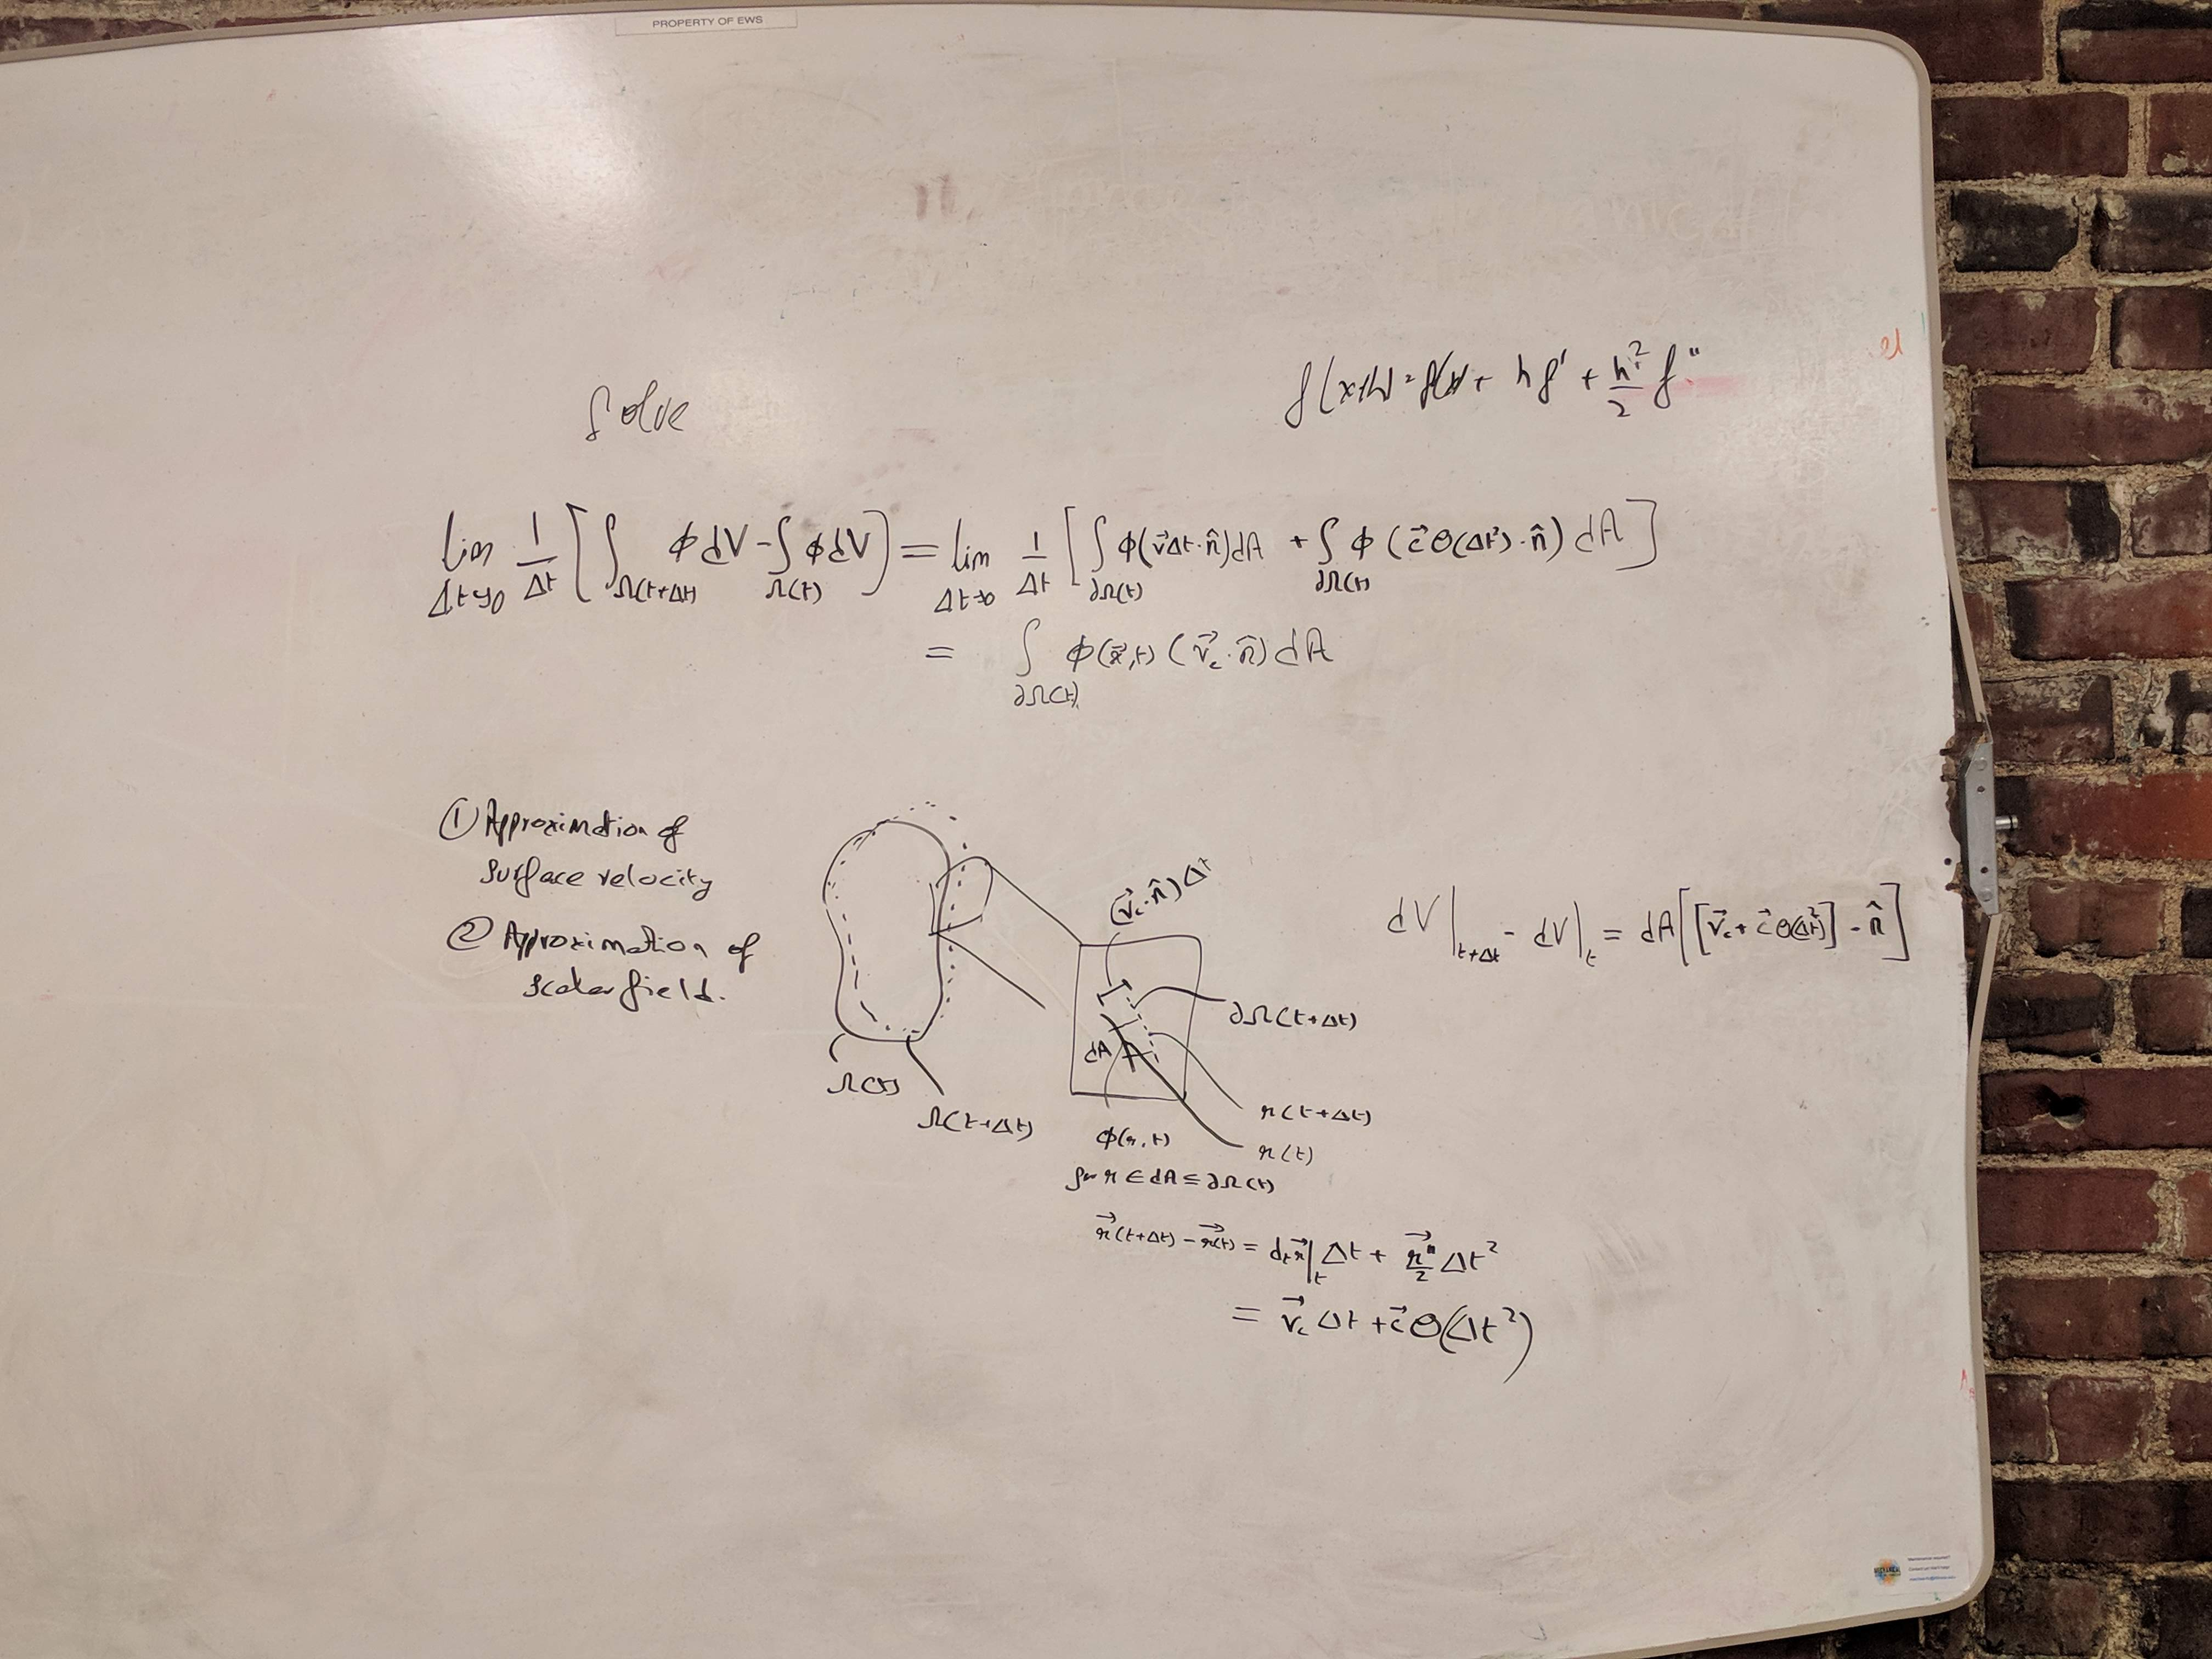
\includegraphics[width=1.0\textwidth]{fig/RTT.jpg}
    \caption{Evaluating Key Limit in RTT Proof}
    \label{fig:rtt}
\end{figure}

\begin{figure}[h!]
    \centering
    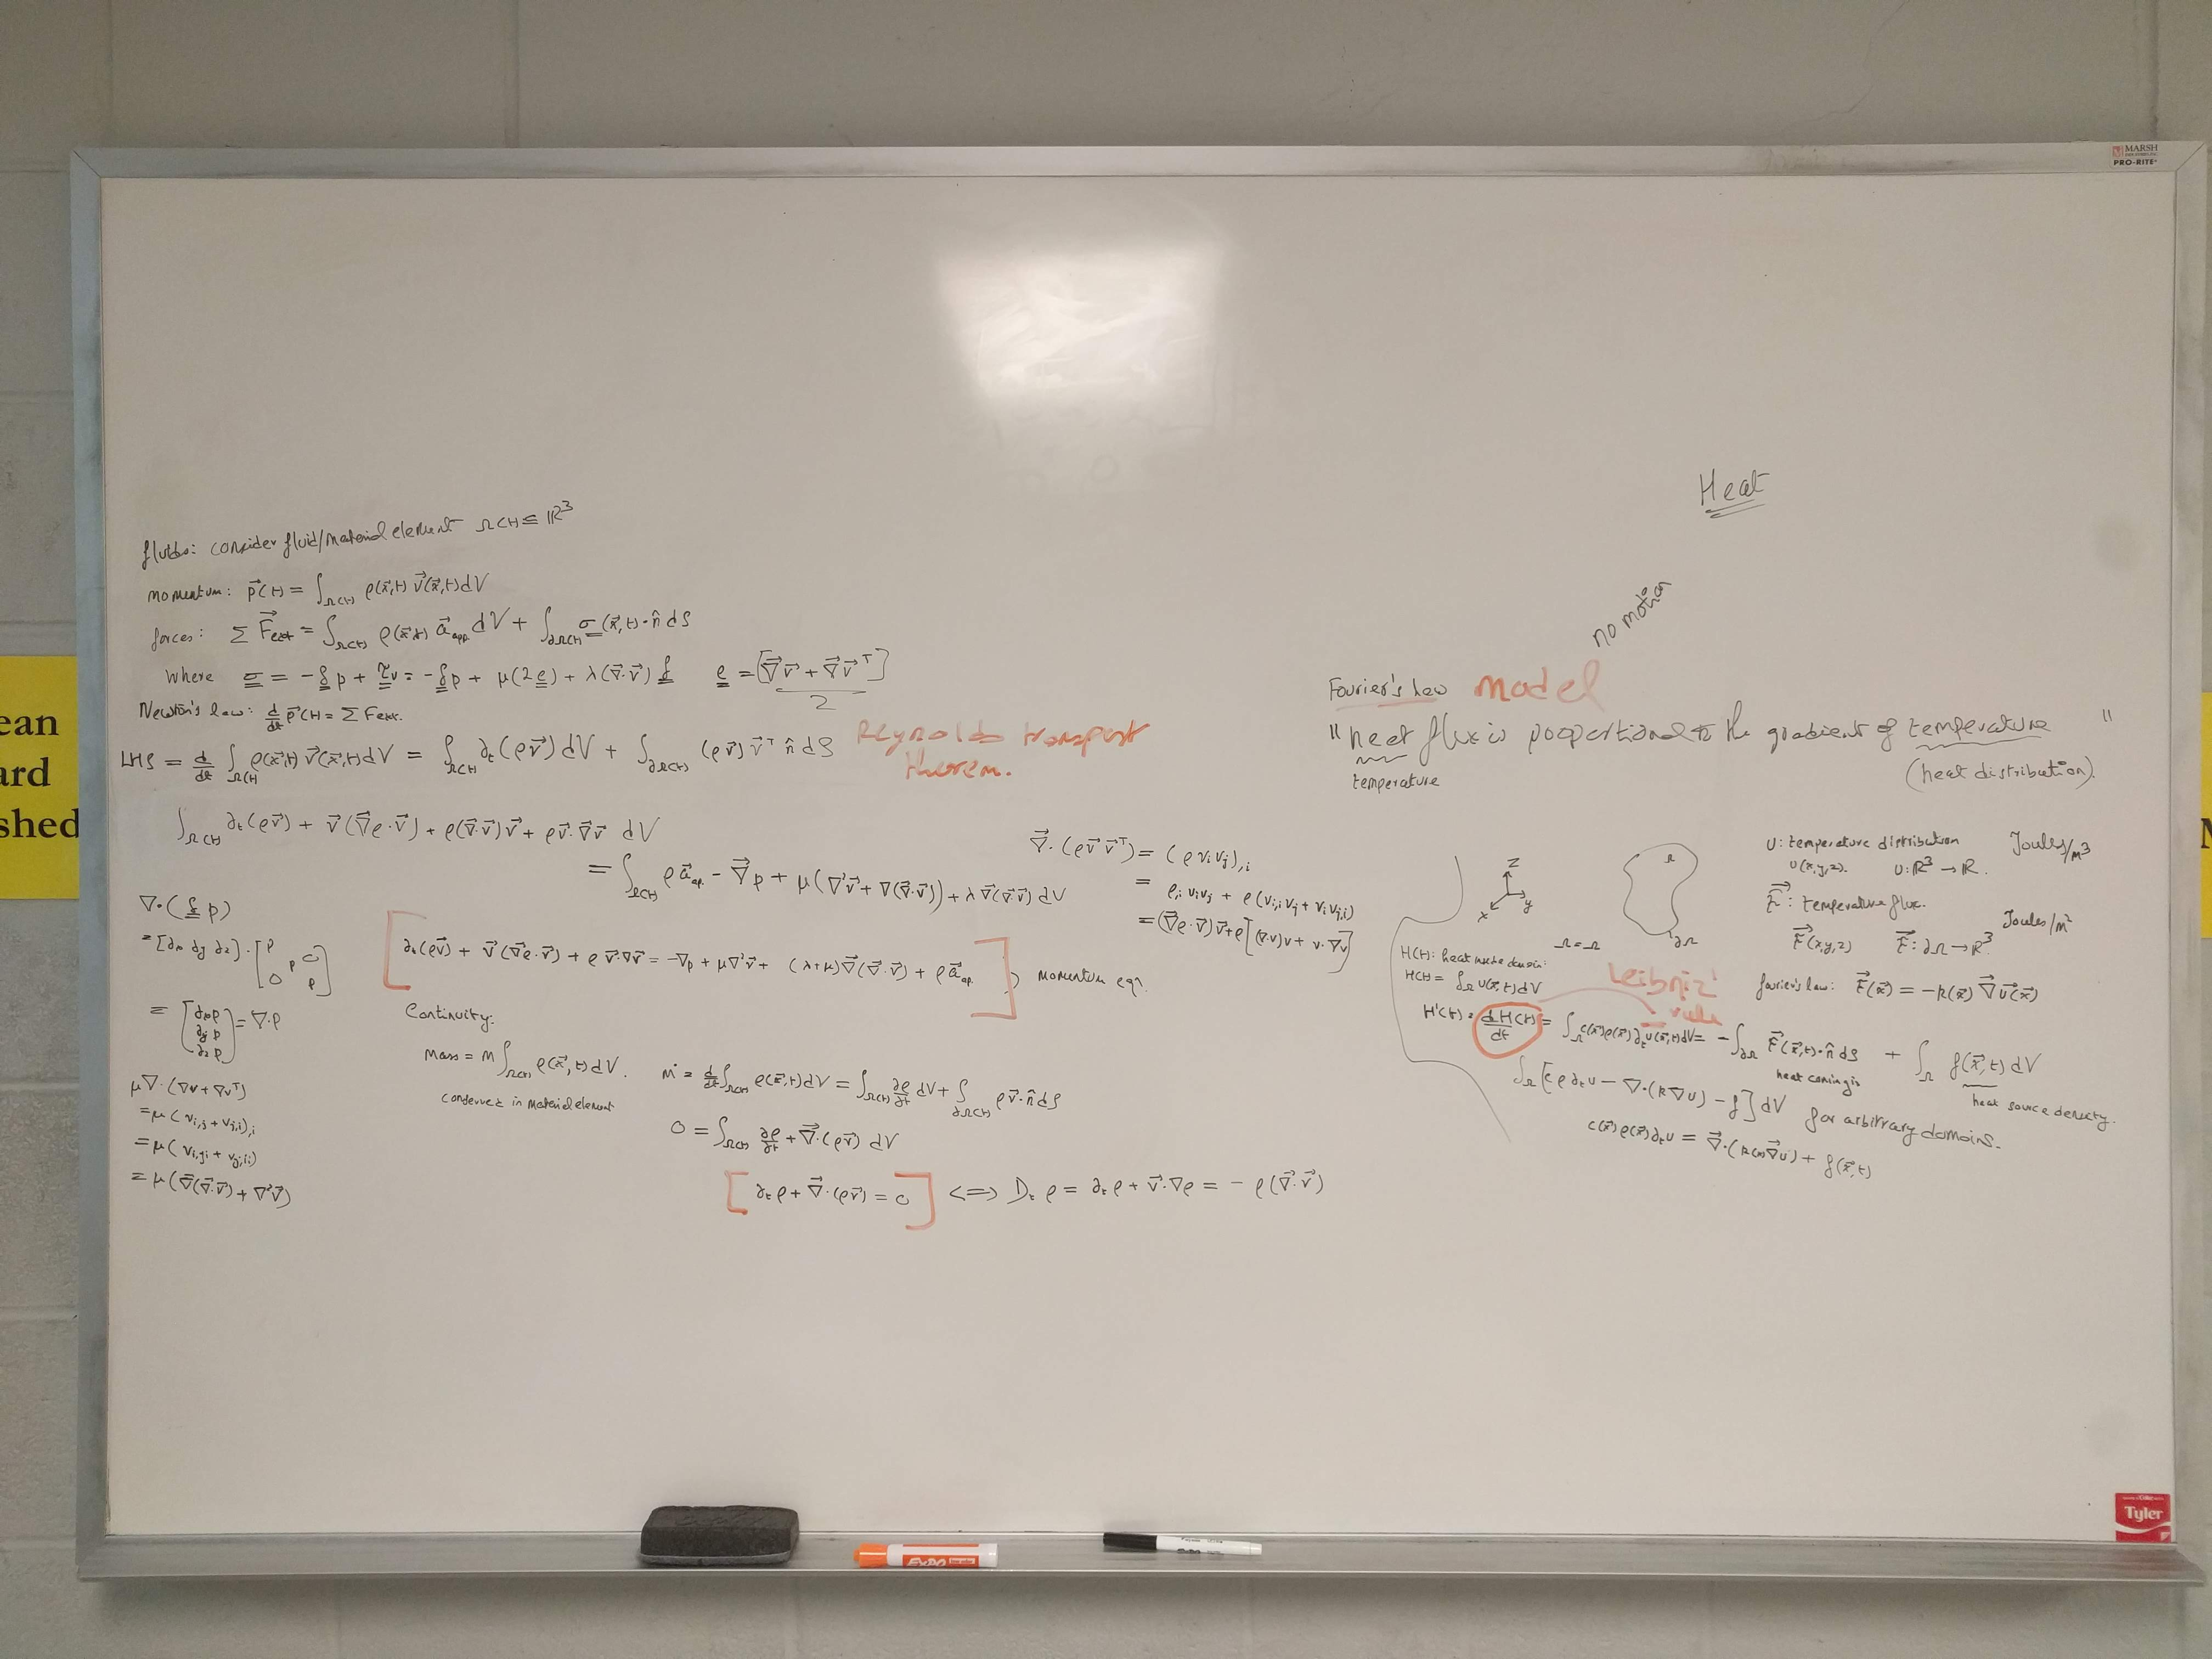
\includegraphics[width=1.0\textwidth]{fig/NS.jpg}
    \caption{Navier-Stokes for Compressible Flow}
    \label{fig:ns}
\end{figure}

\chapter{Sobolev Spaces}
more stuff


\end{document}